%%%%%%%%%%%%%%%%%%%%%%%%%%%%%%%%%%%%%%%%%
% Masters/Doctoral Thesis 
% LaTeX Template
% Version 2.5 (27/8/17)
%
% This template was downloaded from:
% http://www.LaTeXTemplates.com
%
% Version 2.x major modifications by:
% Vel (vel@latextemplates.com)
%
% This template is based on a template by:
% Steve Gunn (http://users.ecs.soton.ac.uk/srg/softwaretools/document/templates/)
% Sunil Patel (http://www.sunilpatel.co.uk/thesis-template/)
%
% Template license:
% CC BY-NC-SA 3.0 (http://creativecommons.org/licenses/by-nc-sa/3.0/)
%
%%%%%%%%%%%%%%%%%%%%%%%%%%%%%%%%%%%%%%%%%

\PassOptionsToPackage{english}{babel}

%----------------------------------------------------------------------------------------
%	PACKAGES AND OTHER DOCUMENT CONFIGURATIONS
%----------------------------------------------------------------------------------------

\documentclass[
12pt, % The default document font size, options: 10pt, 11pt, 12pt
%oneside,Two side (alternating margins) for binding by default, uncomment to switch to one side
english, % ngerman for German
singlespacing, % Single line spacing, alternatives: onehalfspacing or doublespacing
%draft, % Uncomment to enable draft mode (no pictures, no links, overfull hboxes indicated)
%nolistspacing, % If the document is onehalfspacing or doublespacing, uncomment this to set spacing in lists to single
%liststotoc, % Uncomment to add the list of figures/tables/etc to the table of contents
%toctotoc, % Uncomment to add the main table of contents to the table of contents
%parskip, % Uncomment to add space between paragraphs
%nohyperref, % Uncomment to not load the hyperref package
headsepline, % Uncomment to get a line under the header
%chapterinoneline, % Uncomment to place the chapter title next to the number on one line
%consistentlayout, % Uncomment to change the layout of the declaration, abstract and acknowledgements pages to match the default layout
]{MastersDoctoralThesis} % The class file specifying the document structure

\usepackage[utf8]{inputenc} % Required for inputting international characters
\usepackage[T1]{fontenc} % Output font encoding for international characters
\usepackage{mathpazo} % Use the Palatino font by default
\usepackage{graphicx}
\usepackage[backend=bibtex,style=numeric,natbib=true]{biblatex} % Use the bibtex backend with the authoryear citation style (which resembles APA)

\addbibresource{Bibliography/Bibliografia.bib} % The filename of the bibliography

\usepackage[autostyle=true]{csquotes} % Required to generate language-dependent quotes in the bibliography
\usepackage{path}
\usepackage{hyperref}
\usepackage{url}
%\usepackage{gensymb}
\usepackage{wrapfig}
\usepackage{lipsum}
\usepackage{subcaption}
\usepackage{listings}
\DeclareCaptionFormat{listing}{
    \parbox{\textwidth}
  }
\usepackage{siunitx}
\usepackage{csquotes}






%----------------------------------------------------------------------------------------
%	MARGIN SETTINGS
%----------------------------------------------------------------------------------------

\geometry{
	paper=a4paper, % Change to letterpaper for US letter
	inner=2.5cm, % Inner margin
	outer=3.8cm, % Outer margin
	bindingoffset=.5cm, % Binding offset
	top=1.5cm, % Top margin
	bottom=1.5cm, % Bottom margin
	%showframe, % Uncomment to show how the type block is set on the page
}

%----------------------------------------------------------------------------------------
%	THESIS INFORMATION
%----------------------------------------------------------------------------------------





\thesistitle{Open-Source Workflow for the Use of 3D Printing in Dentistry} % Your thesis title, this is used in the title and abstract, print it elsewhere with \ttitle
\supervisor{Prof. Pietro \textsc{Messina}} % Your supervisor's name, this is used in the title page, print it elsewhere with \supname
\examiner{} % Your examiner's name, this is not currently used anywhere in the template, print it elsewhere with \examname
\degree{Laurea Magistrale in Odontoiatria e Protesi Dentaria} % Your degree name, this is used in the title page and abstract, print it elsewhere with \degreename
\author{Calogero \textsc{Carlino}} % Your name, this is used in the title page and abstract, print it elsewhere with \authorname
\addresses{} % Your address, this is not currently used anywhere in the template, print it elsewhere with \addressname

\subject{Odontoiatria e Protesi Dentaria} % Your subject area, this is not currently used anywhere in the template, print it elsewhere with \subjectname
\keywords{} % Keywords for your thesis, this is not currently used anywhere in the template, print it elsewhere with \keywordnames
\university{\href{http://www.unipa.it/}{Università degli Studi di Palermo}} % Your university's name and URL, this is used in the title page and abstract, print it elsewhere with \univname
\department{\href{http://www.unipa.it/dipartimenti/di.chir.on.s.}{Dipartimento Discipline Chirurgiche, Oncologiche e Stomatologiche}} % Your department's name and URL, this is used in the title page and abstract, print it elsewhere with \deptname
%\group{\href{http://researchgroup.university.com}{Research Group Name}} % Your research group's name and URL, this is used in the title page, print it elsewhere with \groupname
%\faculty{\href{http://faculty.university.com}{Faculty Name}} % Your faculty's name and URL, this is used in the title page and abstract, print it elsewhere with \facname

\AtBeginDocument{
\hypersetup{pdftitle=\ttitle} % Set the PDF's title to your title
\hypersetup{pdfauthor=\authorname} % Set the PDF's author to your name
\hypersetup{pdfkeywords=\keywordnames} % Set the PDF's keywords to your keywords
}

\begin{document}

\frontmatter % Use roman page numbering style (i, ii, iii, iv...) for the pre-content pages

\pagestyle{plain} % Default to the plain heading style until the thesis style is called for the body content

%----------------------------------------------------------------------------------------
%	TITLE PAGE
%----------------------------------------------------------------------------------------

\begin{titlepage}
\begin{center}

%unipa logo rescaled and centered
\begin{figure}

\includegraphics[width=\textwidth,height=\textheight,keepaspectratio]{logo_Unipa}
\label{fig:logo_Unipa}
\end{figure}

%\vspace*{.02\textheight}
%{\scshape\LARGE \univname\par}\vspace{1.5cm} % University name
%\textsc{\Large Tesi di Laure Magistrale a Ciclo Unico}\\[0.5cm] % Thesis type

\begin{center}
\textsc{Scuola di Medicina e Chirurgia}
\end{center}

\begin{center}
Corso di Laurea in Odontoiatria e Protesi Dentaria \\
Dipartimento delle Discipline Chirurgiche, Oncologiche e Stomatologiche
\end{center}


\HRule \\[0.4cm] % Horizontal line
{\huge \bfseries \ttitle\par}\vspace{0.4cm} % Thesis title
\HRule \\[1.5cm] % Horizontal line
 
\begin{minipage}[t]{0.4\textwidth}
\begin{flushleft} \large
\emph{Tesi di Laurea di:}\\
\href{}{\textbf{\authorname}} % Author name - remove the \href bracket to remove the link
\end{flushleft}
\end{minipage}
\begin{minipage}[t]{0.4\textwidth}
\begin{flushright} \large
\emph{Relatore:} \\
\href{}{\textbf{\supname}} % Supervisor name - remove the \href bracket to remove the link  
\end{flushright}
\end{minipage}\\[2cm]
 
%\vfill

%\large \textit{A thesis submitted in fulfillment of the requirements\\ for the degree of \degreename}\\[0.3cm] % University requirement text
%\textit{in the}\\[0.4cm]
%\groupname\\\deptname\\[2cm] % Research group name and department name
 
%\vfill

%{\large \today}\\[4cm] % Date
%\includegraphics{Logo} % University/department logo - uncomment to place it

\begin{center}
\large{Anno Accademico 2017-2018}
\end{center}

%magistrale logo
\begin{figure}[b]
\centering

\includegraphics[width=\textwidth,height=\textheight,keepaspectratio]{magistralecicloUnico}
\label{fig:magistralecicloUnico}
\end{figure}
 
\vfill

\end{center}
\end{titlepage}

%----------------------------------------------------------------------------------------
%	DECLARATION PAGE
%----------------------------------------------------------------------------------------

%\begin{declaration}
%\addchaptertocentry{\authorshipname} % Add the declaration to the table of contents
%\noindent I, \authorname, declare that this thesis titled, \enquote{\ttitle} and the work presented in it are my own. I confirm that:

%\begin{itemize} 
%\item This work was done wholly or mainly while in candidature for a research degree at this University.
%\item Where any part of this thesis has previously been submitted for a degree or any other qualification at this University or any other institution, this has been clearly stated.
%\item Where I have consulted the published work of others, this is always clearly attributed.
%\item Where I have quoted from the work of others, the source is always given. With the exception of such quotations, this thesis is entirely my own work.
%\item I have acknowledged all main sources of help.
%\item Where the thesis is based on work done by myself jointly with others, I have made clear exactly what was done by others and what I have contributed myself.\\
%\end{itemize}
 
%\noindent Signed:\\
%\rule[0.5em]{25em}{0.5pt} % This prints a line for the signature
 
%\noindent Date:\\
%\rule[0.5em]{25em}{0.5pt} % This prints a line to write the date
%\end{declaration}

%\cleardoublepage

%----------------------------------------------------------------------------------------
%	QUOTATION PAGE
%----------------------------------------------------------------------------------------

%\vspace*{0.2\textheight}

%\noindent\enquote{\itshape Thanks to my solid academic training, today I can write hundreds of words on virtually any topic without possessing a shred of information, which is how I got a good job in journalism.}\bigbreak

%\hfill Dave Barry

%----------------------------------------------------------------------------------------
%	ABSTRACT PAGE
%----------------------------------------------------------------------------------------

%\begin{abstract}
%\addchaptertocentry{\abstractname} % Add the abstract to the table of contents
%The Thesis Abstract is written here (and usually kept to just this page). The page is kept centered vertically so can expand into the blank space above the title too\ldots
%\end{abstract}

%--------------------------
% License
%\chapter{License} % Main chapter title

\label{Copyright} % Change X to a consecutive number; for referencing this chapter elsewhere, use \ref{ChapterX}

%------------------------------------
    Copyright (C)  2018 - Calogero Carlino.\\
    Permission is granted to copy, distribute and/or modify this document
    under the terms of the GNU Free Documentation License, Version 1.3
    or any later version published by the Free Software Foundation;
    with no Invariant Sections, no Front-Cover Texts, and no Back-Cover Texts.
    A copy of the license is included in the section entitled "GNU
    Free Documentation License".


%----------------------------------------------------------------------------------------
%	LIST OF CONTENTS/FIGURES/TABLES PAGES
%----------------------------------------------------------------------------------------

\tableofcontents % Prints the main table of contents

%\listoffigures % Prints the list of figures

%%\listoftables % Prints the list of tables

%----------------------------------------------------------------------------------------
%	ABBREVIATIONS
%----------------------------------------------------------------------------------------


%\begin{abbreviations}{ll} % Include a list of abbreviations (a table of two columns)

%\textbf{LAH} & \textbf{L}ist \textbf{A}bbreviations \textbf{H}ere\\
%\textbf{WSF} & \textbf{W}hat (it) \textbf{S}tands \textbf{F}or\\

%\end{abbreviations}

%----------------------------------------------------------------------------------------
%	PHYSICAL CONSTANTS/OTHER DEFINITIONS
%----------------------------------------------------------------------------------------

%\begin{constants}{lr@{${}={}$}l} % The list of physical constants is a three column table

% The \SI{}{} command is provided by the siunitx package, see its documentation for instructions on how to use it

%Speed of Light & $c_{0}$ & \SI{2.99792458e8}{\meter\per\second} (exact)\\
%Constant Name & $Symbol$ & $Constant Value$ with units\\

%\end{constants}

%----------------------------------------------------------------------------------------
%	SYMBOLS
%----------------------------------------------------------------------------------------

%\begin{symbols}{lll} % Include a list of Symbols (a three column table)

%$a$ & distance & \si{\meter} \\
%$P$ & power & \si{\watt} (\si{\joule\per\second}) \\
%Symbol & Name & Unit \\

%\addlinespace % Gap to separate the Roman symbols from the Greek

%$\omega$ & angular frequency & \si{\radian} \\

%\end{symbols}

%----------------------------------------------------------------------------------------
%	DEDICATION
%----------------------------------------------------------------------------------------

%\dedicatory{A \\zia Rossella zio Totò nonna Carmela nonno Calogero} 


%----------------------------------------------------------------------------------------
%	ACKNOWLEDGEMENTS
%----------------------------------------------------------------------------------------

%% Chapter Template

\chapter{Ringraziamenti} % Main chapter title

\label{Ringraziamenti} % Change X to a consecutive number; for referencing this chapter elsewhere, use \ref{ChapterX}
 
 %----------------------------------------------------
 
 Un mio caro amico disse una volta che i sentimenti che si provano verso le persone, se messi nero su bianco non sono comparabili a quelli che si possono raccontare con le parole.\\

Ed io sono d'accordo con lui.\\

Quindi cosa sono queste righe? Ecco, queste righe sono come una foto. Una come le tante che ognuno di noi ha, salvata sul cellulare o stampata ed attaccata su un album fatto a mano con amore.
Queste righe catturano ciò che sento in questo momento per delle persone speciali, che in tanti modi mi sono state vicine in questi anni. Persone con cui ho condiviso momenti che porto nel cuore e che, nonostante tutto, sono ancora qui.
Non mi spiego ancora come facciano a restare, ma sono sicuro che hanno una pazienza incredibile.
Le foto in generale mi piacciono, ma ne ho poche perché raramente mi viene in mente di scattarne.
Quindi vi chiedo di concedermi una foto alternativa.\\

\emph{\textbf{E sorridete, che se no viene male!}}\\


%Con ognuno di voi ho condiviso la pezzi di vita durante questi anni di università. Alcuni vi conoscevo da prima, altri vi ho incontrati durante questo percorso. Ho ricordi di così tanti momenti con voi che si affollano nella mia mente, e in tutti vedo la felicità, l'amicizia e l'amore. Vorrei raccontarvi ogni cosa che ho vissuto con ognuno di voi, ma alla fine mi rendo conto che non ha senso. Non ha senso perché voi già sapete tutto, perché voi eravate li con me in quei momenti.\\

Il primo grazie è per \textbf{i miei genitori}, che continuano sempre a supportarmi nel mio percorso. È grazie a voi che mi ritrovo a scrivere queste righe. Avete sempre messo il nostro bene al centro della famiglia ed è a voi che mi ispiro pensando al futuro. Questo traguardo è vostro più di quanto sia mio, che avete instancabilmente lavorato affinché potesse realizzarsi. Grazie, di tutto!\\

Un ringraziamento va al \textbf{Prof Messina}, che mi ha dato fiducia nella realizzazione di questo progetto di tesi e per i consigli preziosi che mi ha fornito nel corso della sperimentazione e nella stesura. La ringrazio anche per ciò che mi ha trasmesso nel corso di questi anni di università, soprattutto per il metodo di analisi clinica e per avermi mostrato quanto sia importante il rapporto di fiducia tra medico e paziente. \\

\textbf{Pasky}, dovrei ringraziarti per infinite cose, per esserci sempre stato, per le chiacchierate sempre appassionate, per le partite alla Play, i film, la musica e milioni di altre cose; ma alla fine tu lo sai già fratè, queste righe non rendono giustizia. \\

Un ringraziamento è di dovere per \textbf{Rossella}, che negli ultimi anni mi è stata vicina e mi ha incoraggiato ad espandere la mia quotidianità con nuove idee e progetti per il futuro. Il tempo trascorso insieme, seppure non sia mai abbastanza, è sempre ricco di amore, felicità e leggerezza, e per questo è la cosa più preziosa.\\

Grazie anche a miei \textbf{amici e coinquilini} con cui ho condiviso la gran parte della mia permanenza a Palermo. Se tutto è andato bene alla fine, è anche perché tutto è iniziato per il meglio in quella casa in via Marinuzzi 100.\\

Un grazie speciale va a \textbf{Salvo}, che negli ultimi vent'anni c'è sempre stato, per tutto. Se facessi l'elenco di tutte le cose che abbiamo fatto insieme (anche solo di quelle poche che ricordo) questi ringraziamenti sarebbero più lunghi della tesi. Se poi inserissi i progetti abbozzati insieme, bhe a quel punto non basterebbe la carta della copisteria. So che non ci tieni a sti ringraziamenti e magari starai già ridendo, ma io li metto uguale, anche per ricordarmi che dobbiamo aumentare il numero di progetti che portiamo dalla teoria alla pratica! ;)\\

Un altro grazie va alla \emph{\textbf{Disagio House}} ed il popolo che le gravita attorno. Nonostante mi intrufolassi nella casa per diversi giorni, mi avete sempre accolto con un sorriso gentile e con grandi quantità di prelibata pizza bianca e birre artigianali. Io provando a ricambiare vi ho donato delle splendide polpettine alla menta, che poi penso siano state riproposte dalla Colgate per qualche campagna anti-alitosi\ldots in ogni caso vi cedo il Copyright.
Il caso ha voluto che le sessioni di laurea combaciassero nei nostri rispettivi Atenei, per cui non posso che rinnovare i miei migliori auguri a voi nuovi dottori. Ci vediamo presto!\\



\emph{\textbf{Un grande grazie va a tutti i miei colleghi e amici, senza i quali questi anni non sarebbero stati così ricchi di bei momenti.}}\\

\textbf{Tommaso}, grazie per le tue freddure e per i brindisi che abbiamo condiviso. Grazie per le ballate sui tavoli e per avermi raccontato di storia, cultura e religione, facendomi apprezzare ogni angolo di questa città e della nostra tradizione.\\

\textbf{Giovanna}, grazie per la tua (vitale) assistenza organizzativa e per tutte le risate fatte a lezione. Grazie per tutti i brindisi fatti insieme, mentre studiavamo da qualche sbob a me incomprensibile, ma tu avevi sempre tutto pronto, bello ordinato e colorato. Grazie amica, per aver condiviso con me le variegate esperienze di questi anni e per avermi reso una persona migliore.\\

\textbf{Martina}, grazie per le birre e il cibo a qualunque orario, per i video stupidi che abbiamo condiviso e per tutti i passaggi che mi hai dato in questi anni. Grazie per la tua generosità e gentilezza e per il continuo impegno che metti in quello che fai, che siano impegni universitari e professionali o la lotta per la legalità e l'uguaglianza sociale. Non cambiare mai. E grazie per avermi fatto conoscere Andrea, nonostante ciò che continua a dire Giovanna. ;)\\

\textbf{Giuliana}, grazie per il tuo cuore palermitano puro in un vestito da principessa. Grazie per le tue imitazioni e per tutte le volte che millantavi di non sapere nulla dell'esame e puntualmente te ne uscivi con una lode. Grazie per esserci sempre, che sia per un caffè, una pizza (sugo di pomodoro, crudo e scaglie) o un'ansia preesame (che ormai sono finiti! :D ) . E grazie per avermi fatto conoscere una persona speciale come Valerio, sempre pronto per un brindisi e generoso nei consigli.\\

\textbf{Giorgia}, grazie per i negroni, le profonde chiacchierate ed i tuoi giochi improvvisati. Grazie per essere sempre sincera e gentile e per impegnarti sempre ad essere migliore giorno dopo giorno. Migliore lo sei già e rendi migliore chi ti sta intorno.\\

\textbf{Cinzia}, grazie per la tua simpatia e sincerità, per i fotobrodi e le birre alla spina. Grazie per i tuoi consigli e il tuo supporto. Grazie per aver alleviato le lezioni ed i tirocini con ironia e spensieratezza. E grazie anche per avermi fatto conoscere il caro Vicio.\\

\textbf{Peppino e Angelo}, gli ultimi banchi sono una tradizione, così come la fame improvvisa durante le sale operatorie e le pizze mangiate fuori dall'aula. Avete alleggerito quelle aule ripiene di estrogeni ed evidenziatori colorati, e per questo non posso fare a meno di dirvi grazie.\\


A huge thank you to \textbf{my Munich family}, friends who I never hoped to find and that instead made me go through an unforgettable year. This project is also yours! Thanks for the time that we spent together, for the parties, for the BBQ in the garden and at the lake, for the lectures that we attended and for the always interesting discussions that we did about any topic! Thanks for the nights at the Blitz and for every time that you entered in my room with someting to eat. We passed good and bad times, but we were always together, like a Family. Thanks Bros, love you all!\\

\pagebreak

Un ultimo ringraziamento lo devo fare non ad una persona in particolare, ma a tutte le persone che ho incontrato nella mia vita, docenti, parenti, professionisti, che mi hanno detto che c'era qualcosa che non avrei potuto fare, perché non ne sarei stato in grado, perché avrei fatto brutta figura, perché non è quello che ci si aspetta\ldots Questo sarà anche vero nella maggior parte dei casi, ma provare è una mia scelta, una scelta che ognuno ha, perché ognuno è libero di provare e fallire, per poi provare ancora.\\
Sono felice di non aver dato ascolto a queste voci, sono felice di aver sbagliato molte più volte di quelle che mi avevano detto che avrei sbagliato. Perché così facendo ho imparato a far tesoro di ogni sbaglio.\\ Grazie a chi non ha creduto in me, siete stati la molla che mi ha fatto andare avanti ogni volta che non avrei più voluto farlo.\\ Non date retta a chi dice che non siete in grado di fare qualcosa che voi ardentemente volete, ma impiegate le vostre energie per raggiungere l'obiettivo.\\

\emph{\textbf{La nostra vita è solo nostra, non lasciamo che altri ne decidano il percorso}}.



 




%----------------------------------------------------------------------------------------
%	Introduction
%----------------------------------------------------------------------------------------

% Chapter Template

\chapter{Introduction} % Main chapter title

\label{Introduzione} % Change X to a consecutive number; for referencing this chapter elsewhere, use \ref{ChapterX}
 
 %----------------------------------------------------
 
 
This work was made to give an insight into the use of \emph{medical modeling} and of its dental applications in combination with additive manufacturing technologies, which have potential for significant impact on clinical practice and dental research.\\
The digital management of medical diagnostic images is treated focusing on the practical use, through the use of segmentation software and extraction of three-dimensional digital models of parts of the human organism. There is an overview on the management of digital models to obtain, through the 3D printing process, real three-dimensional models of anatomical parts and pathological lesions.\\
Diagnostic images processing is a process that generates a large amount of data, which can be further processed to improve patient management and treatment. The three-dimensional visualization of the patient's reconstructions gives the physician an in-depth view of the clinical situation, and makes it possible to design accurate and often minimally invasive treatment plans. The clinical researcher can now use various technologies to analyze images and produce physical object, which serve as an aid to diagnosis and therapy.\\
Concepts of \emph{computer vision} and \emph{computer graphics} make possible the visualization of images and 3D reconstructions, as well as the production and advanced elaboration of the models. Modern additive manufacturing techniques bring the virtual model into reality, using various materials to generate real models from digital counterparts. There is therefore the possibility to touch the patient's reconstructions, for a better study of the case, for a better explanation of the treatment plan to the patient and for the planning of surgical interventions.\\
The additive manufacturing in the medical field goes beyond the printing of models made of thermoplastic material. Biofabrication is a recent discipline which, using specific tools for additive manufacturing and knowledge gained in the fields of regenerative medicine and tissue engineering, aims to reproduce in vitro tissues and organs of the human organism, which can be implanted on patients instead of prostheses or organs taken from donors. \\
A good diagnosis starts with the analysis of patient data. With the growth of data available on large numbers of patients, at the populations level, it is difficult for the human being to find every correlation between them. For this reason, algorithms have been developed to correlate and classify data. The use of this amount of information can have serious implications in research, among all in the pharmacological research and in the research of molecular markers of disease and tumors. \\
This amalgamation of technologies gives to the doctor, today more than ever, the opportunity to provide the patient with a treatment of excellence, from the diagnosis to the follow-up. Although the learning curve for the use of some of the software and technologies used here is steep, the possibilities that they provide for personalizing patient treatment are relevant. \\
The aim of this work is also to make the workflow as consistent as possible with the ideals of the \emph{Free Software Foundation} (FSF), to facilitate the adoption of the procedures described here and to give a small contribution to the diffusion of knowledge and awareness of a field with strong potential for the protection of human health.


%----------------------------------------------------------------------------------------
%	THESIS CONTENT - CHAPTERS
%----------------------------------------------------------------------------------------

\mainmatter % Begin numeric (1,2,3...) page numbering

\pagestyle{thesis} % Return the page headers back to the "thesis" style

% Include the chapters of the thesis as separate files from the Chapters folder
% Uncomment the lines as you write the chapters
%% Chapter 1

\chapter{Chapter Title Here} % Main chapter title

\label{ChapterSpiegazione} % For referencing the chapter elsewhere, use \ref{Chapter1} 

%----------------------------------------------------------------------------------------

% Define some commands to keep the formatting separated from the content 
\newcommand{\keyword}[1]{\textbf{#1}}
\newcommand{\tabhead}[1]{\textbf{#1}}
\newcommand{\code}[1]{\texttt{#1}}
\newcommand{\file}[1]{\texttt{\bfseries#1}}
\newcommand{\option}[1]{\texttt{\itshape#1}}

%----------------------------------------------------------------------------------------

\section{Welcome and Thank You}
Welcome to this \LaTeX{} Thesis Template, a beautiful and easy to use template for writing a thesis using the \LaTeX{} typesetting system.

If you are writing a thesis (or will be in the future) and its subject is technical or mathematical (though it doesn't have to be), then creating it in \LaTeX{} is highly recommended as a way to make sure you can just get down to the essential writing without having to worry over formatting or wasting time arguing with your word processor. 

\LaTeX{} is easily able to professionally typeset documents that run to hundreds or thousands of pages long. With simple mark-up commands, it automatically sets out the table of contents, margins, page headers and footers and keeps the formatting consistent and beautiful. One of its main strengths is the way it can easily typeset mathematics, even \emph{heavy} mathematics. Even if those equations are the most horribly twisted and most difficult mathematical problems that can only be solved on a super-computer, you can at least count on \LaTeX{} to make them look stunning.

%----------------------------------------------------------------------------------------

\section{Learning \LaTeX{}}

\LaTeX{} is not a \textsc{wysiwyg} (What You See is What You Get) program, unlike word processors such as Microsoft Word or Apple's Pages. Instead, a document written for \LaTeX{} is actually a simple, plain text file that contains \emph{no formatting}. You tell \LaTeX{} how you want the formatting in the finished document by writing in simple commands amongst the text, for example, if I want to use \emph{italic text for emphasis}, I write the \verb|\emph{text}| command and put the text I want in italics in between the curly braces. This means that \LaTeX{} is a \enquote{mark-up} language, very much like HTML.

\subsection{A (not so short) Introduction to \LaTeX{}}

If you are new to \LaTeX{}, there is a very good eBook -- freely available online as a PDF file -- called, \enquote{The Not So Short Introduction to \LaTeX{}}. The book's title is typically shortened to just \emph{lshort}. You can download the latest version (as it is occasionally updated) from here:
\url{http://www.ctan.org/tex-archive/info/lshort/english/lshort.pdf}

It is also available in several other languages. Find yours from the list on this page: \url{http://www.ctan.org/tex-archive/info/lshort/}

It is recommended to take a little time out to learn how to use \LaTeX{} by creating several, small `test' documents, or having a close look at several templates on:\\ 
\url{http://www.LaTeXTemplates.com}\\ 
Making the effort now means you're not stuck learning the system when what you \emph{really} need to be doing is writing your thesis.

\subsection{A Short Math Guide for \LaTeX{}}

If you are writing a technical or mathematical thesis, then you may want to read the document by the AMS (American Mathematical Society) called, \enquote{A Short Math Guide for \LaTeX{}}. It can be found online here:
\url{http://www.ams.org/tex/amslatex.html}
under the \enquote{Additional Documentation} section towards the bottom of the page.

\subsection{Common \LaTeX{} Math Symbols}
There are a multitude of mathematical symbols available for \LaTeX{} and it would take a great effort to learn the commands for them all. The most common ones you are likely to use are shown on this page:
\url{http://www.sunilpatel.co.uk/latex-type/latex-math-symbols/}

You can use this page as a reference or crib sheet, the symbols are rendered as large, high quality images so you can quickly find the \LaTeX{} command for the symbol you need.

\subsection{\LaTeX{} on a Mac}
 
The \LaTeX{} distribution is available for many systems including Windows, Linux and Mac OS X. The package for OS X is called MacTeX and it contains all the applications you need -- bundled together and pre-customized -- for a fully working \LaTeX{} environment and work flow.
 
MacTeX includes a custom dedicated \LaTeX{} editor called TeXShop for writing your `\file{.tex}' files and BibDesk: a program to manage your references and create your bibliography section just as easily as managing songs and creating playlists in iTunes.

%----------------------------------------------------------------------------------------

\section{Getting Started with this Template}

If you are familiar with \LaTeX{}, then you should explore the directory structure of the template and then proceed to place your own information into the \emph{THESIS INFORMATION} block of the \file{main.tex} file. You can then modify the rest of this file to your unique specifications based on your degree/university. Section \ref{FillingFile} on page \pageref{FillingFile} will help you do this. Make sure you also read section \ref{ThesisConventions} about thesis conventions to get the most out of this template.

If you are new to \LaTeX{} it is recommended that you carry on reading through the rest of the information in this document.

Before you begin using this template you should ensure that its style complies with the thesis style guidelines imposed by your institution. In most cases this template style and layout will be suitable. If it is not, it may only require a small change to bring the template in line with your institution's recommendations. These modifications will need to be done on the \file{MastersDoctoralThesis.cls} file.

\subsection{About this Template}

This \LaTeX{} Thesis Template is originally based and created around a \LaTeX{} style file created by Steve R.\ Gunn from the University of Southampton (UK), department of Electronics and Computer Science. You can find his original thesis style file at his site, here:
\url{http://www.ecs.soton.ac.uk/~srg/softwaretools/document/templates/}

Steve's \file{ecsthesis.cls} was then taken by Sunil Patel who modified it by creating a skeleton framework and folder structure to place the thesis files in. The resulting template can be found on Sunil's site here:
\url{http://www.sunilpatel.co.uk/thesis-template}

Sunil's template was made available through \url{http://www.LaTeXTemplates.com} where it was modified many times based on user requests and questions. Version 2.0 and onwards of this template represents a major modification to Sunil's template and is, in fact, hardly recognisable. The work to make version 2.0 possible was carried out by \href{mailto:vel@latextemplates.com}{Vel} and Johannes Böttcher.

%----------------------------------------------------------------------------------------

\section{What this Template Includes}

\subsection{Folders}

This template comes as a single zip file that expands out to several files and folders. The folder names are mostly self-explanatory:

\keyword{Appendices} -- this is the folder where you put the appendices. Each appendix should go into its own separate \file{.tex} file. An example and template are included in the directory.

\keyword{Chapters} -- this is the folder where you put the thesis chapters. A thesis usually has about six chapters, though there is no hard rule on this. Each chapter should go in its own separate \file{.tex} file and they can be split as:
\begin{itemize}
\item Chapter 1: Introduction to the thesis topic
\item Chapter 2: Background information and theory
\item Chapter 3: (Laboratory) experimental setup
\item Chapter 4: Details of experiment 1
\item Chapter 5: Details of experiment 2
\item Chapter 6: Discussion of the experimental results
\item Chapter 7: Conclusion and future directions
\end{itemize}
This chapter layout is specialised for the experimental sciences, your discipline may be different.

\keyword{Figures} -- this folder contains all figures for the thesis. These are the final images that will go into the thesis document.

\subsection{Files}

Included are also several files, most of them are plain text and you can see their contents in a text editor. After initial compilation, you will see that more auxiliary files are created by \LaTeX{} or BibTeX and which you don't need to delete or worry about:

\keyword{example.bib} -- this is an important file that contains all the bibliographic information and references that you will be citing in the thesis for use with BibTeX. You can write it manually, but there are reference manager programs available that will create and manage it for you. Bibliographies in \LaTeX{} are a large subject and you may need to read about BibTeX before starting with this. Many modern reference managers will allow you to export your references in BibTeX format which greatly eases the amount of work you have to do.

\keyword{MastersDoctoralThesis.cls} -- this is an important file. It is the class file that tells \LaTeX{} how to format the thesis. 

\keyword{main.pdf} -- this is your beautifully typeset thesis (in the PDF file format) created by \LaTeX{}. It is supplied in the PDF with the template and after you compile the template you should get an identical version.

\keyword{main.tex} -- this is an important file. This is the file that you tell \LaTeX{} to compile to produce your thesis as a PDF file. It contains the framework and constructs that tell \LaTeX{} how to layout the thesis. It is heavily commented so you can read exactly what each line of code does and why it is there. After you put your own information into the \emph{THESIS INFORMATION} block -- you have now started your thesis!

Files that are \emph{not} included, but are created by \LaTeX{} as auxiliary files include:

\keyword{main.aux} -- this is an auxiliary file generated by \LaTeX{}, if it is deleted \LaTeX{} simply regenerates it when you run the main \file{.tex} file.

\keyword{main.bbl} -- this is an auxiliary file generated by BibTeX, if it is deleted, BibTeX simply regenerates it when you run the \file{main.aux} file. Whereas the \file{.bib} file contains all the references you have, this \file{.bbl} file contains the references you have actually cited in the thesis and is used to build the bibliography section of the thesis.

\keyword{main.blg} -- this is an auxiliary file generated by BibTeX, if it is deleted BibTeX simply regenerates it when you run the main \file{.aux} file.

\keyword{main.lof} -- this is an auxiliary file generated by \LaTeX{}, if it is deleted \LaTeX{} simply regenerates it when you run the main \file{.tex} file. It tells \LaTeX{} how to build the \emph{List of Figures} section.

\keyword{main.log} -- this is an auxiliary file generated by \LaTeX{}, if it is deleted \LaTeX{} simply regenerates it when you run the main \file{.tex} file. It contains messages from \LaTeX{}, if you receive errors and warnings from \LaTeX{}, they will be in this \file{.log} file.

\keyword{main.lot} -- this is an auxiliary file generated by \LaTeX{}, if it is deleted \LaTeX{} simply regenerates it when you run the main \file{.tex} file. It tells \LaTeX{} how to build the \emph{List of Tables} section.

\keyword{main.out} -- this is an auxiliary file generated by \LaTeX{}, if it is deleted \LaTeX{} simply regenerates it when you run the main \file{.tex} file.

So from this long list, only the files with the \file{.bib}, \file{.cls} and \file{.tex} extensions are the most important ones. The other auxiliary files can be ignored or deleted as \LaTeX{} and BibTeX will regenerate them.

%----------------------------------------------------------------------------------------

\section{Filling in Your Information in the \file{main.tex} File}\label{FillingFile}

You will need to personalise the thesis template and make it your own by filling in your own information. This is done by editing the \file{main.tex} file in a text editor or your favourite LaTeX environment.

Open the file and scroll down to the third large block titled \emph{THESIS INFORMATION} where you can see the entries for \emph{University Name}, \emph{Department Name}, etc \ldots

Fill out the information about yourself, your group and institution. You can also insert web links, if you do, make sure you use the full URL, including the \code{http://} for this. If you don't want these to be linked, simply remove the \verb|\href{url}{name}| and only leave the name.

When you have done this, save the file and recompile \code{main.tex}. All the information you filled in should now be in the PDF, complete with web links. You can now begin your thesis proper!

%----------------------------------------------------------------------------------------

\section{The \code{main.tex} File Explained}

The \file{main.tex} file contains the structure of the thesis. There are plenty of written comments that explain what pages, sections and formatting the \LaTeX{} code is creating. Each major document element is divided into commented blocks with titles in all capitals to make it obvious what the following bit of code is doing. Initially there seems to be a lot of \LaTeX{} code, but this is all formatting, and it has all been taken care of so you don't have to do it.

Begin by checking that your information on the title page is correct. For the thesis declaration, your institution may insist on something different than the text given. If this is the case, just replace what you see with what is required in the \emph{DECLARATION PAGE} block.

Then comes a page which contains a funny quote. You can put your own, or quote your favourite scientist, author, person, and so on. Make sure to put the name of the person who you took the quote from.

Following this is the abstract page which summarises your work in a condensed way and can almost be used as a standalone document to describe what you have done. The text you write will cause the heading to move up so don't worry about running out of space.

Next come the acknowledgements. On this page, write about all the people who you wish to thank (not forgetting parents, partners and your advisor/supervisor).

The contents pages, list of figures and tables are all taken care of for you and do not need to be manually created or edited. The next set of pages are more likely to be optional and can be deleted since they are for a more technical thesis: insert a list of abbreviations you have used in the thesis, then a list of the physical constants and numbers you refer to and finally, a list of mathematical symbols used in any formulae. Making the effort to fill these tables means the reader has a one-stop place to refer to instead of searching the internet and references to try and find out what you meant by certain abbreviations or symbols.

The list of symbols is split into the Roman and Greek alphabets. Whereas the abbreviations and symbols ought to be listed in alphabetical order (and this is \emph{not} done automatically for you) the list of physical constants should be grouped into similar themes.

The next page contains a one line dedication. Who will you dedicate your thesis to?

Finally, there is the block where the chapters are included. Uncomment the lines (delete the \code{\%} character) as you write the chapters. Each chapter should be written in its own file and put into the \emph{Chapters} folder and named \file{Chapter1}, \file{Chapter2}, etc\ldots Similarly for the appendices, uncomment the lines as you need them. Each appendix should go into its own file and placed in the \emph{Appendices} folder.

After the preamble, chapters and appendices finally comes the bibliography. The bibliography style (called \option{authoryear}) is used for the bibliography and is a fully featured style that will even include links to where the referenced paper can be found online. Do not underestimate how grateful your reader will be to find that a reference to a paper is just a click away. Of course, this relies on you putting the URL information into the BibTeX file in the first place.

%----------------------------------------------------------------------------------------

\section{Thesis Features and Conventions}\label{ThesisConventions}

To get the best out of this template, there are a few conventions that you may want to follow.

One of the most important (and most difficult) things to keep track of in such a long document as a thesis is consistency. Using certain conventions and ways of doing things (such as using a Todo list) makes the job easier. Of course, all of these are optional and you can adopt your own method.

\subsection{Printing Format}

This thesis template is designed for double sided printing (i.e. content on the front and back of pages) as most theses are printed and bound this way. Switching to one sided printing is as simple as uncommenting the \option{oneside} option of the \code{documentclass} command at the top of the \file{main.tex} file. You may then wish to adjust the margins to suit specifications from your institution.

The headers for the pages contain the page number on the outer side (so it is easy to flick through to the page you want) and the chapter name on the inner side.

The text is set to 11 point by default with single line spacing, again, you can tune the text size and spacing should you want or need to using the options at the very start of \file{main.tex}. The spacing can be changed similarly by replacing the \option{singlespacing} with \option{onehalfspacing} or \option{doublespacing}.

\subsection{Using US Letter Paper}

The paper size used in the template is A4, which is the standard size in Europe. If you are using this thesis template elsewhere and particularly in the United States, then you may have to change the A4 paper size to the US Letter size. This can be done in the margins settings section in \file{main.tex}.

Due to the differences in the paper size, the resulting margins may be different to what you like or require (as it is common for institutions to dictate certain margin sizes). If this is the case, then the margin sizes can be tweaked by modifying the values in the same block as where you set the paper size. Now your document should be set up for US Letter paper size with suitable margins.

\subsection{References}

The \code{biblatex} package is used to format the bibliography and inserts references such as this one \parencite{Reference1}. The options used in the \file{main.tex} file mean that the in-text citations of references are formatted with the author(s) listed with the date of the publication. Multiple references are separated by semicolons (e.g. \parencite{Reference2, Reference1}) and references with more than three authors only show the first author with \emph{et al.} indicating there are more authors (e.g. \parencite{Reference3}). This is done automatically for you. To see how you use references, have a look at the \file{Chapter1.tex} source file. Many reference managers allow you to simply drag the reference into the document as you type.

Scientific references should come \emph{before} the punctuation mark if there is one (such as a comma or period). The same goes for footnotes\footnote{Such as this footnote, here down at the bottom of the page.}. You can change this but the most important thing is to keep the convention consistent throughout the thesis. Footnotes themselves should be full, descriptive sentences (beginning with a capital letter and ending with a full stop). The APA6 states: \enquote{Footnote numbers should be superscripted, [...], following any punctuation mark except a dash.} The Chicago manual of style states: \enquote{A note number should be placed at the end of a sentence or clause. The number follows any punctuation mark except the dash, which it precedes. It follows a closing parenthesis.}

The bibliography is typeset with references listed in alphabetical order by the first author's last name. This is similar to the APA referencing style. To see how \LaTeX{} typesets the bibliography, have a look at the very end of this document (or just click on the reference number links in in-text citations).

\subsubsection{A Note on bibtex}

The bibtex backend used in the template by default does not correctly handle unicode character encoding (i.e. "international" characters). You may see a warning about this in the compilation log and, if your references contain unicode characters, they may not show up correctly or at all. The solution to this is to use the biber backend instead of the outdated bibtex backend. This is done by finding this in \file{main.tex}: \option{backend=bibtex} and changing it to \option{backend=biber}. You will then need to delete all auxiliary BibTeX files and navigate to the template directory in your terminal (command prompt). Once there, simply type \code{biber main} and biber will compile your bibliography. You can then compile \file{main.tex} as normal and your bibliography will be updated. An alternative is to set up your LaTeX editor to compile with biber instead of bibtex, see \href{http://tex.stackexchange.com/questions/154751/biblatex-with-biber-configuring-my-editor-to-avoid-undefined-citations/}{here} for how to do this for various editors.

\subsection{Tables}

Tables are an important way of displaying your results, below is an example table which was generated with this code:

{\small
\begin{verbatim}
\begin{table}
\caption{The effects of treatments X and Y on the four groups studied.}
\label{tab:treatments}
\centering
\begin{tabular}{l l l}
\toprule
\tabhead{Groups} & \tabhead{Treatment X} & \tabhead{Treatment Y} \\
\midrule
1 & 0.2 & 0.8\\
2 & 0.17 & 0.7\\
3 & 0.24 & 0.75\\
4 & 0.68 & 0.3\\
\bottomrule\\
\end{tabular}
\end{table}
\end{verbatim}
}

\begin{table}
\caption{The effects of treatments X and Y on the four groups studied.}
\label{tab:treatments}
\centering
\begin{tabular}{l l l}
\toprule
\tabhead{Groups} & \tabhead{Treatment X} & \tabhead{Treatment Y} \\
\midrule
1 & 0.2 & 0.8\\
2 & 0.17 & 0.7\\
3 & 0.24 & 0.75\\
4 & 0.68 & 0.3\\
\bottomrule\\
\end{tabular}
\end{table}

You can reference tables with \verb|\ref{<label>}| where the label is defined within the table environment. See \file{Chapter1.tex} for an example of the label and citation (e.g. Table~\ref{tab:treatments}).

\subsection{Figures}

There will hopefully be many figures in your thesis (that should be placed in the \emph{Figures} folder). The way to insert figures into your thesis is to use a code template like this:
\begin{verbatim}
\begin{figure}
\centering

\includegraphics{Figures/Electron}
\decoRule
\caption[An Electron]{An electron (artist's impression).}
\label{fig:Electron}
\end{figure}
\end{verbatim}
Also look in the source file. Putting this code into the source file produces the picture of the electron that you can see in the figure below.

\begin{figure}[th]
\centering

\includegraphics{Figures/Electron}
\decoRule
\caption[An Electron]{An electron (artist's impression).}
\label{fig:Electron}
\end{figure}

Sometimes figures don't always appear where you write them in the source. The placement depends on how much space there is on the page for the figure. Sometimes there is not enough room to fit a figure directly where it should go (in relation to the text) and so \LaTeX{} puts it at the top of the next page. Positioning figures is the job of \LaTeX{} and so you should only worry about making them look good!

Figures usually should have captions just in case you need to refer to them (such as in Figure~\ref{fig:Electron}). The \verb|\caption| command contains two parts, the first part, inside the square brackets is the title that will appear in the \emph{List of Figures}, and so should be short. The second part in the curly brackets should contain the longer and more descriptive caption text.

The \verb|\decoRule| command is optional and simply puts an aesthetic horizontal line below the image. If you do this for one image, do it for all of them.

\LaTeX{} is capable of using images in pdf, jpg and png format.

\subsection{Typesetting mathematics}

If your thesis is going to contain heavy mathematical content, be sure that \LaTeX{} will make it look beautiful, even though it won't be able to solve the equations for you.

The \enquote{Not So Short Introduction to \LaTeX} (available on \href{http://www.ctan.org/tex-archive/info/lshort/english/lshort.pdf}{CTAN}) should tell you everything you need to know for most cases of typesetting mathematics. If you need more information, a much more thorough mathematical guide is available from the AMS called, \enquote{A Short Math Guide to \LaTeX} and can be downloaded from:
\url{ftp://ftp.ams.org/pub/tex/doc/amsmath/short-math-guide.pdf}

There are many different \LaTeX{} symbols to remember, luckily you can find the most common symbols in \href{http://ctan.org/pkg/comprehensive}{The Comprehensive \LaTeX~Symbol List}.

You can write an equation, which is automatically given an equation number by \LaTeX{} like this:
\begin{verbatim}
\begin{equation}
E = mc^{2}
\label{eqn:Einstein}
\end{equation}
\end{verbatim}

This will produce Einstein's famous energy-matter equivalence equation:
\begin{equation}
E = mc^{2}
\label{eqn:Einstein}
\end{equation}

All equations you write (which are not in the middle of paragraph text) are automatically given equation numbers by \LaTeX{}. If you don't want a particular equation numbered, use the unnumbered form:
\begin{verbatim}
\[ a^{2}=4 \]
\end{verbatim}

%----------------------------------------------------------------------------------------

\section{Sectioning and Subsectioning}

You should break your thesis up into nice, bite-sized sections and subsections. \LaTeX{} automatically builds a table of Contents by looking at all the \verb|\chapter{}|, \verb|\section{}|  and \verb|\subsection{}| commands you write in the source.

The Table of Contents should only list the sections to three (3) levels. A \verb|chapter{}| is level zero (0). A \verb|\section{}| is level one (1) and so a \verb|\subsection{}| is level two (2). In your thesis it is likely that you will even use a \verb|subsubsection{}|, which is level three (3). The depth to which the Table of Contents is formatted is set within \file{MastersDoctoralThesis.cls}. If you need this changed, you can do it in \file{main.tex}.

%----------------------------------------------------------------------------------------

\section{In Closing}

You have reached the end of this mini-guide. You can now rename or overwrite this pdf file and begin writing your own \file{Chapter1.tex} and the rest of your thesis. The easy work of setting up the structure and framework has been taken care of for you. It's now your job to fill it out!

Good luck and have lots of fun!

\begin{flushright}
Guide written by ---\\
Sunil Patel: \href{http://www.sunilpatel.co.uk}{www.sunilpatel.co.uk}\\
Vel: \href{http://www.LaTeXTemplates.com}{LaTeXTemplates.com}
\end{flushright}

%\include{Chapter/Template}
%% Chapter Template

\chapter{Introduction} % Main chapter title

\label{Introduzione} % Change X to a consecutive number; for referencing this chapter elsewhere, use \ref{ChapterX}
 
 %----------------------------------------------------
 
 
This work was made to give an insight into the use of \emph{medical modeling} and of its dental applications in combination with additive manufacturing technologies, which have potential for significant impact on clinical practice and dental research.\\
The digital management of medical diagnostic images is treated focusing on the practical use, through the use of segmentation software and extraction of three-dimensional digital models of parts of the human organism. There is an overview on the management of digital models to obtain, through the 3D printing process, real three-dimensional models of anatomical parts and pathological lesions.\\
Diagnostic images processing is a process that generates a large amount of data, which can be further processed to improve patient management and treatment. The three-dimensional visualization of the patient's reconstructions gives the physician an in-depth view of the clinical situation, and makes it possible to design accurate and often minimally invasive treatment plans. The clinical researcher can now use various technologies to analyze images and produce physical object, which serve as an aid to diagnosis and therapy.\\
Concepts of \emph{computer vision} and \emph{computer graphics} make possible the visualization of images and 3D reconstructions, as well as the production and advanced elaboration of the models. Modern additive manufacturing techniques bring the virtual model into reality, using various materials to generate real models from digital counterparts. There is therefore the possibility to touch the patient's reconstructions, for a better study of the case, for a better explanation of the treatment plan to the patient and for the planning of surgical interventions.\\
The additive manufacturing in the medical field goes beyond the printing of models made of thermoplastic material. Biofabrication is a recent discipline which, using specific tools for additive manufacturing and knowledge gained in the fields of regenerative medicine and tissue engineering, aims to reproduce in vitro tissues and organs of the human organism, which can be implanted on patients instead of prostheses or organs taken from donors. \\
A good diagnosis starts with the analysis of patient data. With the growth of data available on large numbers of patients, at the populations level, it is difficult for the human being to find every correlation between them. For this reason, algorithms have been developed to correlate and classify data. The use of this amount of information can have serious implications in research, among all in the pharmacological research and in the research of molecular markers of disease and tumors. \\
This amalgamation of technologies gives to the doctor, today more than ever, the opportunity to provide the patient with a treatment of excellence, from the diagnosis to the follow-up. Although the learning curve for the use of some of the software and technologies used here is steep, the possibilities that they provide for personalizing patient treatment are relevant. \\
The aim of this work is also to make the workflow as consistent as possible with the ideals of the \emph{Free Software Foundation} (FSF), to facilitate the adoption of the procedures described here and to give a small contribution to the diffusion of knowledge and awareness of a field with strong potential for the protection of human health.

% Chapter Template

\chapter{Free (Libre) Software} % Main chapter title

\label{Capitolo1} % Change X to a consecutive number; for referencing this chapter elsewhere, use \ref{ChapterX}
 
 %----------------------------------------------------
In the current software landscape, there are various licenses that regulate software's intellectual property and describe the conditions of use and redistribution. Generally we distinguish software with commercial licenses and software with free licenses. \\
The idea of free software comes from \emph{Richard Stallman}, MIT researcher, in 1983, with the aim of creating, distributing and maintaining free software that can be used by all users \parencite{Reference57}, as opposed to software under commercial license that began to be born in those years.\\
Stallman has subsequently founded the \emph{Free Software Foundation}, which is a non-profit organization committed to pursuing the idea and principles of free software \parencite{Reference58}. The FSF also draws free licenses for the protection of copyright; free software is in fact a licensed software, which sets rules on its modification and distribution that ensure that the software continues to be free. \\ There are several free licenses produced by the FSF \parencite{Reference59} and by other entities \parencite{Reference60}, the most common being the GPLv3 \parencite{Reference61}.\\
The use of GPL licenses guarantees that the software released will always be a free software, regardless of changes and redistribution. This is called \emph{Copyleft} and guarantees the freedom of users, opposing to the Copyright.\\
A free license is defined as such if it complies with the \textbf{four freedoms} described by the FSF: \\
\begin{itemize}
\item freedom to use the software for any desired purpose, by any user, on any desired device;
\item freedom to access the source code and to study and modify the software according to your needs;
\item freedom to distribute to the software with whom you want;
\item freedom to distribute the changes made to the software in the way you want, even without Copyleft, but without the obligation to release in non-free form.
\end{itemize}
Software that meets these requirements is called free software. \\
Free software is different from \emph{open-source} software, as in free software there is a strong reference to ethics and freedom of use, while open-source licenses focus on accessibility to source code, which is nevertheless a requirement of free software.

\section{Why to use free software?}
The use of free software is encouraged wherever possible in this manuscript, for the guaranteed freedoms and because it is considered appropriate to make this work widely available and reusable. Finding software at no cost facilitates, in our case, the exploration of alternative routes for the use of diagnostic images, while the \emph{Rep-Rap} project \parencite{Reference62} allow free use of the information regarding additive manufacturing instruments. \\
The freedom to adapt existing hardware and software relieves the users from recreating basic functions, which are already tested in the existing tools, and allows them to focus on solving the specific problem.
In our case many open source software does not contain specific functions for dentistry, and some neither for the medical field in general. With the available source code however, it is possible to make changes or write new functions that allow a fast progression from idea to experimentation (for example \parencite{Reference63}, \parencite{Reference64}). This type of freedom is greatly reduced in commercial software, in which the integration of new functions is possible only by the software manufacturer. \\
Open source software is also often supported by communities of users who contribute to the quality of software, and anyone can check the source code to validate its security, and in the case of flaws, these can be often quickly fixed.\\
Free and open manuscripts are part of general knowledge, to help any user who needs them. They must therefore be preserved and expanded, to ensure that knowledge is not lost, and instead it is made more accessible to accelerate the general process of improvement to which the human beings boldly aims.
% Chapter Template

\chapter{ Medical Imaging} % Main chapter title

\label{Chapter2} % Change X to a consecutive number; for referencing this chapter elsewhere, use \ref{ChapterX}
 
 %----------------------------------------------------
 
 
Radiology gave to the physician a look of the inside the human body without the need for surgery. Images diagnostics has evolved over time, with the introduction of new imaging tools, protocols and imaging technologies based on the use of ionizing radiation and other physical principles. The current diagnostic equipment are accurate, smaller and emits less radiation than before . Moreover, the most recent tools allow to acquire diagnostic data in digital form, enabling data post-processing using dedicated software. Diagnostic images have gone from having only a diagnostic function to being often the basis for the treatment planning.
At the basis of modern digital diagnostics is the \textbf{DICOM} standard (\emph{\textbf{D}igital \textbf{I}maging and \textbf{CO}munication in \textbf{M}edicine}). The standard is freely available online, it can be freely used \parencite{Reference27}. On this Standard is based the whole chain of modern patient management, from the acquisition of clinical and anamnestic data to diagnostic images, up to the transfer of data between different health workers \parencite{Reference25}.

\section{Scanning of the human body}
The human organism is a three-dimensional object oriented in space. In anatomy we describe the human organism located in the \emph{Anatomical Position}.\\
Scanning of the human organism can be performed with different techniques and tools. The scan can represent only the surface of the organism, or also capture its internal organs.

\subsection{Computer Tomography}
Computer Tomography (CT) is a technique that uses beams of X-rays that pass through the human body and are detected by a scanner, that evaluate the energy absorbed during the path, and therefore the density of the tissues (in Hunsfield Unit). This measurement is performed from various angles on the same plane, and the readings are processed by software, which returns an image that is a map of the density of the scanned organism (\emph{\textbf{slice}}). \\
The image is a grid of \textbf{voxel} (whose resolution depends on various factors, including the device used and the FOV (\emph{Field Of View}), always according to the \emph{ALARA} principle), in which each voxel is represented in a shade of gray proportional to the attenuation of the X ray, by the tissue founded in the represented volume. The slices are acquired, one after the other, at a thickness (\emph{slice thickness}) and a distance (\emph{pitch}, \parencite{Reference23}) that depend on the used tomograph and the implemented scanning protocol. The slices acquired are then ordered to form a images series, and each slice is interpolated with the subsequent, allowing to obtain a real volume.
The volume thus constituted can be studied on arbitrary planes of space, thanks to \emph{multiplanar reconstruction algorithms} (MRP). The volumetric representation thus created is of great importance, because it is the base of modern radiological diagnosis and therapy.

\subsection{Cone Beam Computer Tomography (CBCT)}
CBCT is a technique that uses the same physical principles as CT, but presents differences due to scan procedure and reconstruction algorithms \parencite{Reference12}, \parencite{Reference13}.\\
The CBCT scanner uses a conical beam of X-rays, which is rotated around the region to be scanned (\textbf{ROI} - \emph{region of interest}) and is detected by a sensor, placed orthogonal to the beam. The conical beam allows to acquire a volume during the revolution, so the scans are faster and with a lower dose of radiation absorbed by the patient than a conventional CT \parencite{Reference14}. \\
CBCT equipment is smaller and mechanically less complex than conventional CTs; these characteristics, associated with the scanning speed and the lower cost, have made it widespread, especially in the diagnostic of the oromaxillofacial region. The reduced FOV allows to reduce the absorption of radiation and to provide high resolution 3D reconstructions. Interesting is also the fact that these devices, given their small size, have been used as an intraoperative aid during surgery \parencite{Reference15} and during endodontic therapy procedures in selected cases \parencite{Reference16}. \\ 
The diagnostic images obtained from the CBCT scan is the result of a first processing step, which allow to map in a three-dimensional space the data collected by the detector \parencite{Reference11}. The images collected are processed with algorithms to reduce artifacts due to the scanning process. The scattering \emph{noise} is relevant in the unprocessed images, so it is reduced through an image blur process (\emph{blurring} or \emph{smoothing}), finding a compromise with the preservation of the spatial resolution of the images (which is higher at low levels of blur, ie. when the image is well defined, \emph{edge sharpening}). \\
Of relevance, especially in the implant surgery planning, is the assessment of bone quality in the implant site. Historically, bone density, measured in \emph{Hounsfield Unit} (HU), has been the most used parameter to describe bone quality. Today's CBCT scanners do not give Hounsfield's scale images, but in a \emph{gray scale} (Gray Value, GV) which is the representation of the attenuation of the X-ray signal by the tissues found in the path of the beam. \\ It was shown how the grayscale representation is dependent on the scanner used, as well as being highly variable even in the same device. Differences in the representation of the density can be highlighted between the central and the peripheral area of an image, both on the horizontal and vertical axis. To partially obviate to this problem, the scanner must be calibrated with test samples provided by the manufacturer; variability remains even after calibration \parencite{Reference17}, but is considered acceptable for normal procedures. However, the search for algorithms and techniques to reduce scanning artifacts is one of the fields in which innovations \parencite{Reference19} are most frequently presented.\\
CBCT scaning device use a lower slice-thickness than conventional CT, improving the representation of small details, as the endodontic canal.

\begin{figure}[h]
    \centering
    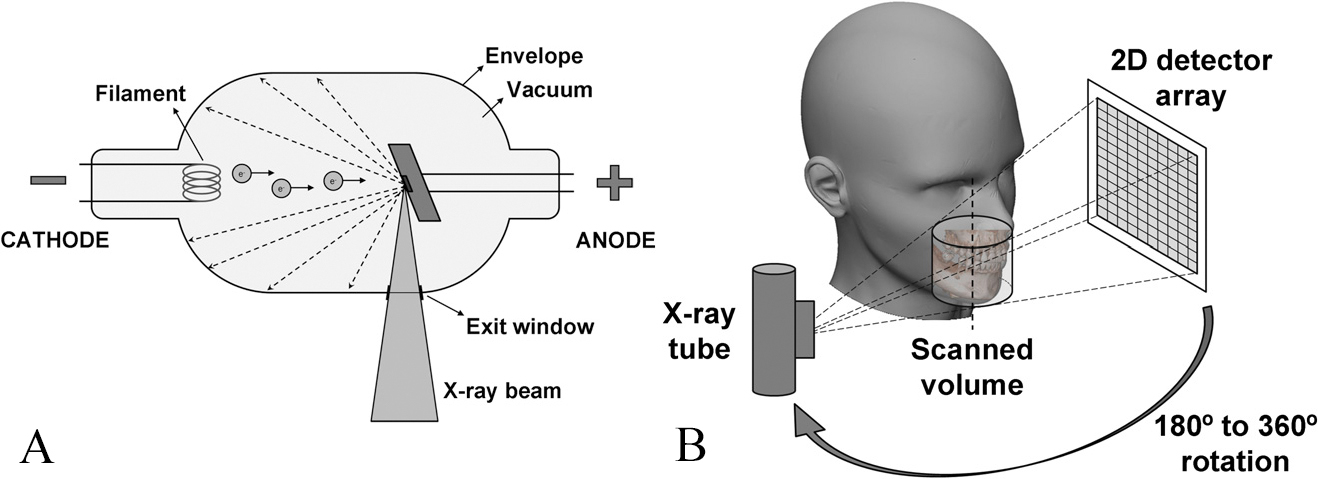
\includegraphics[width =\textwidth, height =\textheight, keepaspectratio]{cbct}
    \caption{\textbf{A}: simplified scheme of a \emph{X-ray tube}. The electric current heats the filament located at the cathode, leading to the release of electrons. The electrons are accelerated towards the anode by means of a potential difference. The collision of electrons on the target leads to the production of X-rays, which are emitted through the exit. The rays in other directions (dotted lines) are attenuated by the tube lining. \textbf{B}: we see the relationship between the X-Ray emitter and the detector, which are placed one in front of the other, and often joined by a C-arm. These two elements make a revolution around the region to be scanned, of an angle between 180 and 360 degrees. From Pauwels et al \parencite{Reference11}.}
    \label{fig: CBCT}
\end{figure}

\subsection{Magnetic Resonance}
Magnetic Resonance Imaging (MRI) uses magnetic fields to orientate water's molecules within the organism and to detect their position, through the energy emitted when they return to their initial configuration, after the magnetic field has been switched off. The scans are repeated to intensify the signal. The image obtained is in grayscale, with the richest areas of water showing a greater intensity (white) than areas with little water (black). MR equipment uses different parameters for detection, with protocols that allow to suppress or increase the signal intensity of a tissue.\\
MRI does not emit ionizing radiation, but it can be risky for the patient with metal implants or pacemakers, so these conditions must be assessed before subjecting the patient to the scan.\\
This imaging technique allows good visualization of the body's soft tissues, but bone margins are difficult to detect, especially at the level of alveolar processes. Some groups have however started to explore the potential of MRI also in the diagnosis of bone pathology \parencite{Reference18} and its microstructure \parencite{Reference19}
\begin{figure}[h]
    \centering
    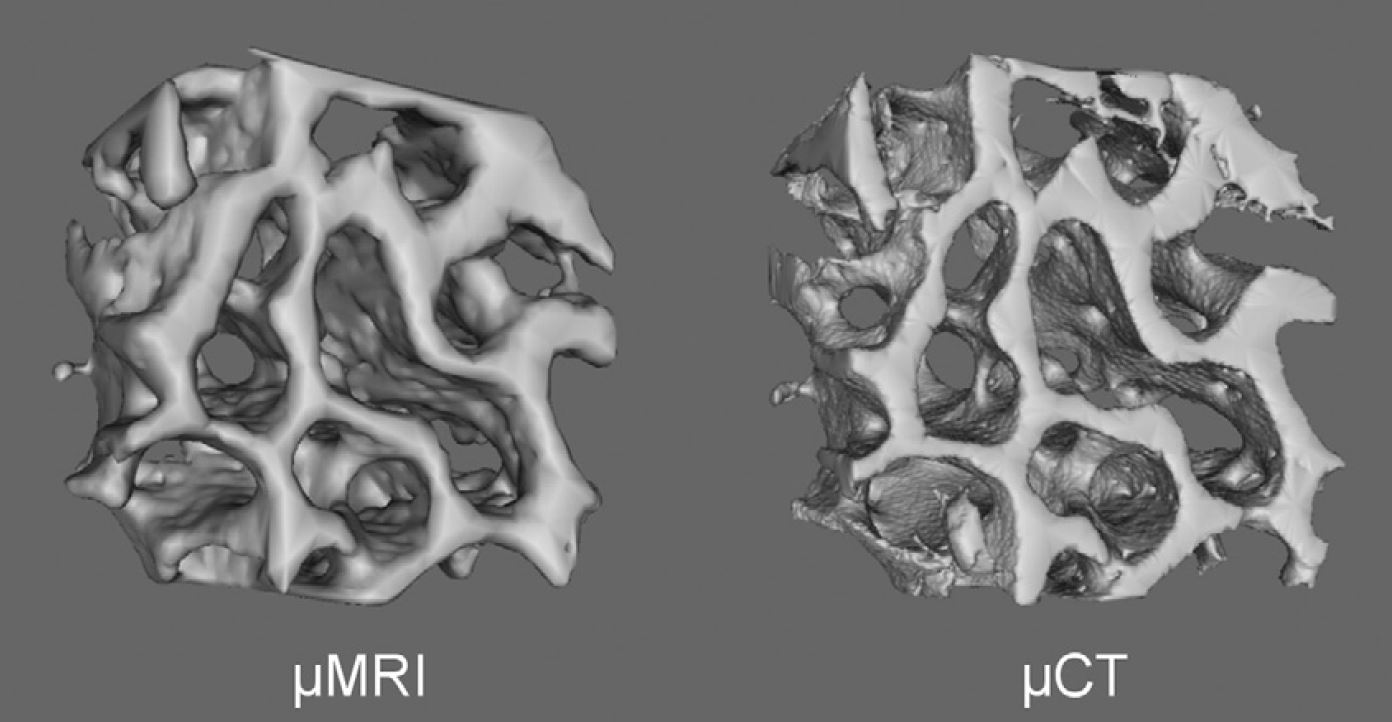
\includegraphics [width=0.5 \textwidth]{trabecole_CTvsMR} 
    \caption{reconstruction of bone trabeculation using two different imaging techniques. From Weiger et al \parencite{Reference19}.}
    \label{fig:trabeculae}
\end{figure}.

\subsection{Surface scans}
Surface scan makes possible to digitize the body surface and the cavities accessible by the scanning equipment.\\
In the dental field various optical scanning devices have spread, replacing the plaster impressions. These scanners allow to obtain digital impressions of the patient's arches, which are important for the subsequent therapy, that very often makes use of CAD/CAM devices for the design and manufacturing of temporary restoration and prosthesis.\\
There are several scanning technologies, but the most used in the medical field are techniques that reconstruct a three-dimensional surface starting from a series of images of the region to be digitized.\\
The instruments required for scanning usually consists of an image acquisition device, a computer and data processing software. The software assists the operator in the images acquisition, which are often processed in real time to provide the clinician with an instant view of the model being acquired. The three-dimensional model thus created can also contain the color of the scanned tissue (\emph{textures}) \parencite{Reference20}. \\
The acquired models can be used in combination with models made by CT or MRI, where the oral tissues are less defined than the models obtained with surface scanners, and may present artifacts due to the presence of prostheses or metal restorations, in addition to not having information of the surface textures. This combination allows the creation of high quality models to accurately plan orthognathic surgery procedures \parencite{Reference21}, \parencite{Reference22}. \\
Digital reconstructions of real objects can also be performed by means of a camera, with a technique called \emph{Photogrammetry}. This consists in acquiring a series of partially superimposed pictures around the object to be scanned; the images are then processed by algorithms to give a digital 3D model \parencite{Reference117}. \newpage
\begin{figure}[h]
\vspace{-10pt}
    \centering
    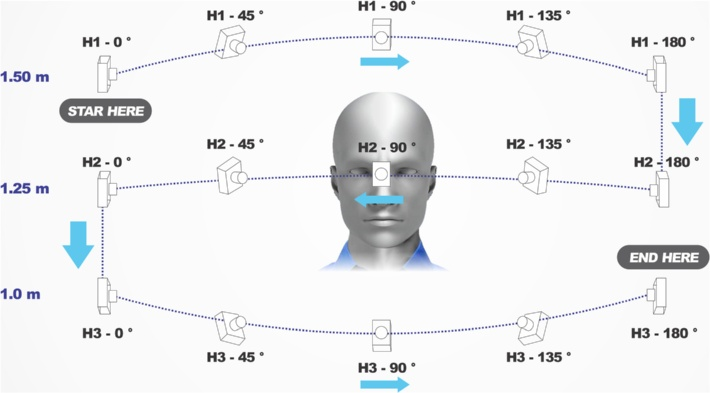
\includegraphics[width=0.8\textwidth, height=\textheight, keepaspectratio]{photogramm_capture}
    \caption{Photogrammetry protocol developed by Salazar-Gamarra et al \parencite{Reference117} for scanning a face using a mobile phone and 123D Catch software (now no longer active).}
    \label{fig:photogramm_capture}
\end{figure}

\section{Problems related to scans}
Digital images share the problem of \emph{\textbf{partial volume effect}}. It consists in the fact that a voxel can represent a single shade of gray, so if in the volume of a voxel there is more than one tissue, perhaps at different densities, the density represented in the voxel will be a weighted average of the densities present in the voxel volume. A decrease in the size of the voxels (and therefore an increase in the number of voxels with the same volume) makes it possible to partially compensate for the problem. \\ This problem is always to be taken into account during image segmentation, because it affects the quality of the details and the discrimination of the boundary of different tissues.
\begin{figure}[h!]
\vspace{-5pt}
    \centering
    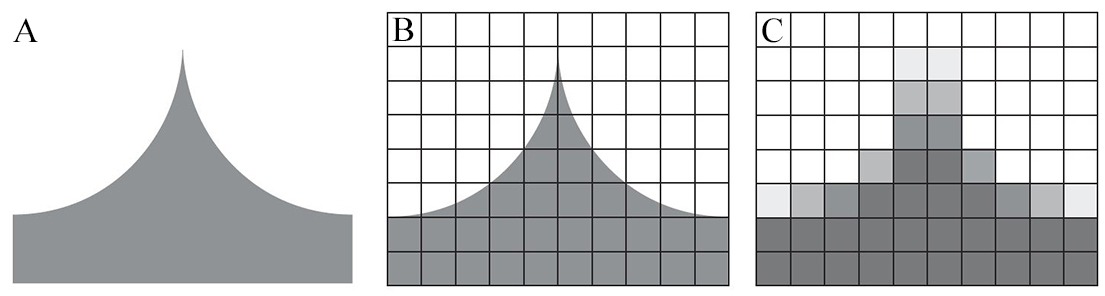
\includegraphics [width = 0.7\textwidth, height =\textheight, keepaspectratio]{black_partial_pixel}
    \caption{Illustration of the partial pixel effect: \textbf{A}: shows the actual shape of the object; \textbf{B}: shows the pixel grid applied to the original shape; \textbf{C} shows the partial pixel effect, where each pixel receives a gray scale according to the average density of the pixel, causing loss of detail. From Bibbs et al \parencite{Reference1}}
    \label{fig: black_partial_pixel}
\vspace{-10pt}
\end{figure}
\\

In optical scans, a frequent problem is the presence of \emph{\textbf{noise}} on the surface of the scan. This is due to various causes, but this problem can be solved with algorithms that calculate the average of the curvature of the surface and remove the points that deviate from it (the variance in the distribution of points is often an adjustable parameter in the cleaning algorithm ).

\begin{figure}[h]
    \centering
    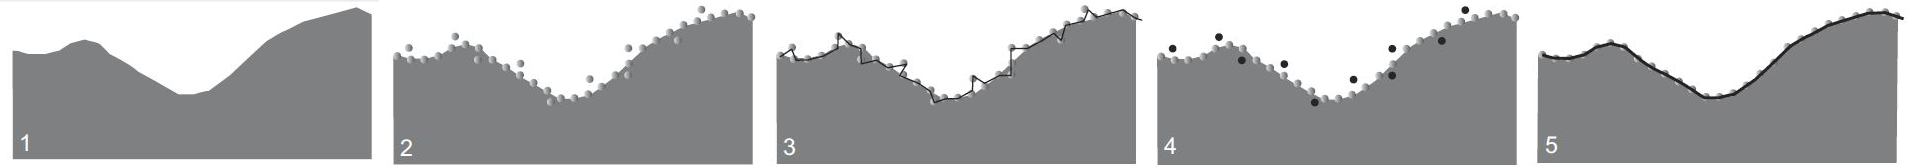
\includegraphics[width=\textwidth, height=\textheight, keepaspectratio]{orizontal_noise}
    \caption{(1) shows the original morphology of the object. (2) shows the reconstruction obtained from the scan. (3) shows the evaluation of the homogeneity of the scan surface. (4) shows the selected points that deviate from the average position of the points on the surface. (5) clean scan (\emph{denoising}). Modified From Bibbs et al \parencite{Reference1}.}
    \label{fig:orizontal_noise}
\end{figure}

\section{The safety of medical images}
DICOM files contain sensitive patient data, such as general information, medical history and diseases, as well as medical images. These files are often sent to colleagues for advice, shared for research purposes or shown to students during teaching. There are online libraries where diagnostic image sets are loaded for research purposes, and these are freely accessible on the web \parencite{Reference24}. To allow a more secure management of images preserving the possibility of sharing, several methods have been proposed. \\
Essential is the protection of patient data in the network in which the data is collected. Computers and servers should be protected by a firewall, while data should only be sent via a VPN. But this is not enough to protect the data when they as to leave the original network. This is why the data must be anonymized or encrypted.

\subsection{Anonymization}
Anonymization consists of removing entries containing sensitive data from the DICOM file. However, the right balance between the data removed for security and those to be maintained must be found, because items such as date of birth, sex and date of execution of the surveys are important both in the subsequent study of the images and for their management.\\
Anonymization is not always necessary if images are to be kept in a private and protected archive, but should be used when the file is spread and there is a risk to the patient's privacy. \\
Several software, open-source or commercial, have been proposed for the scope, for example DICOM Confidential \parencite{Reference46}. \\Anonymisation is an \textbf{irreversible} process, because is impossible to retrieve data after that they have been removed from the DICOM file.

\subsection{Encryption}
Encryption is essentially the process of translating data into another form to prevent them from being easily understood. \\ Replacing every letter of a word with the following letter in the alphabet (hello -> dlbp) is an example of \emph{symmetric key cryptography}, because the key (replacing every letter of the message with the next to encrypt and with the previous one to decipher) is the same for both parties that exchange the message. The \emph{asymmetric key algorithms} work with a key for encryption (\emph{public key}) and a key for decryption (\emph{private key}). \\ \textbf{RSA} is an asymmetric key algorithm, whereas \textbf{AES} is a symmetric key algorithm; both are supported by the DICOM Standard. The choice of the algorithm must however be made not only looking at security, but also at the time of encryption-decryption. RSA is currently considered very safe, but it is also slower to calculate; for this reason RSA is used to generate keys, which is a process that is performed infrequently, while AES is used with RSA keys to encode data \parencite{Reference25}. \\
Encryption is a completely \textbf{reversible} process, so there is no loss of data during the process.

\subsection{Evaluation of data integrity}
There are many ways to exchange data, and this flexibility comes at the risk that the data is somehow changed without permission. To solve this problem we can use another tool borrowed from cryptography: \emph{\textbf{hash function}}. The hash function is essentially an algorithm that takes as \emph{input} an arbitrary sequence of bits, and give as \emph{output} a standard sequence of bit. When the input is changed, there is a very high probability that the output will change. \\
If, for example, in a CT the value of one or more pixels is changed, or the date of acquisition is changed, when the hash is assessed the output will not match the original one, which indicates that given is corrupted. \\
QuickHash GUI is a cross-platform open-source software with a graphical interface, which allows to create hash of files and folders and to check their authenticity \parencite{Reference65}.
\begin{figure}[h]
    \centering
    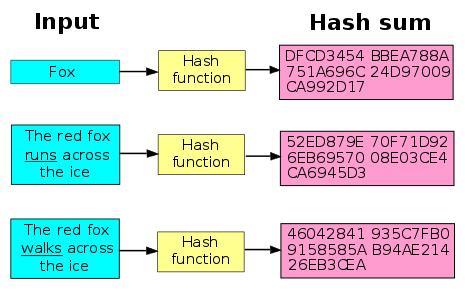
\includegraphics [width=0.6\textwidth, height=\textheight, keepaspectratio]{Hash_function}
    \caption {scheme of a hash function: an input is processed with a hash function, which results in a standardized output. From \emph{Wikipedia}}
    \label{fig:Hash_function}
\end{figure}

\subsection{Evaluating data source}
When two operators exchange data, who receives the data must be sure of the validity of the sender.
With digital data, this confirmation is given by the digital signature. The digital signature is a sequence of characters that is issued by trustworthy entities after ascertaining the credentials of the applicant. The recipient of the data will then be able to discriminate the valid sender based on his signature.

 
% Chapter Template

\chapter{Medical Modeling} % Main chapter title

\label{Chapter3} % Change X to a consecutive number; for referencing this chapter elsewhere, use \ref{ChapterX}
 
 %----------------------------------------------------

Digital modeling and rapid prototyping arise from the engineering need to quickly and cost-effectively design prototypes modeled using CAD software.\\
This request has led to an evolution of the software and equipment necessary to put this workflow into practice. Rapid prototyping has proved to be a useful tool, allowing to quickly evaluate the physical prototype and improve its digital design according to what it is found on the prototype, until a product that meets the required needs is obtained, iteration after iteration. \\
It was then realized that the same concept could be applied to other types of three-dimensional data, leading to the development of software to interface medical scans with rapid prototyping equipment. From the appreciation of the potential of this approach has developed the multidisciplinary field of Medical Modeling, which brings together engineers, radiologists, surgeons, designers, computer scientists and various other professionals, with the aim of using the acquired data from the patients to provide them with the highest standards of therapy \parencite{Reference1}.

\section{What can be done with patient images?}
Diagnostic images are extremely useful, both in everyday clinical practice and in research.
The digitization of acquisitions, the widespread use of computers and the variety of software available for data processing have allowed doctors to integrate imaging diagnostics into their daily activities. Diagnostic instruments are often sold by manufacturers with packages that include dedicated workstations and software. This should ensure, to the professional who buys the package, the full compatibility and integration of the dataflow between the purchased instruments. \\ 
When using medical imaging equipment, we do not work directly with the DICOM standard, but we are dealing with the implementation of the DICOM made by the manufacturer of the instrument used. This means that compatibility is not guaranteed, but we must rely on the \emph{DICOM Conformance Statement} that the manufacturer must attach to the tool, which indicates which functions of the DICOM standard have been implemented \parencite{Reference25}. \\
Proprietary software is certainly efficient, easy to use and often has good performance, especially when used on workstations marketed by the same manufacturer. At the same time these software are often not available outside of the packages comprehensive of the diagnostic equipment, or have a high cost to be purchased by institutions on a budget or by clinicians and students who want to approach the field. In addition, the fact that software is delivered with commercial license means that its source code is not accessible, and researchers working in the field have no way of developing new functions or testing new techniques on these software. \\
For these reasons, several open-source software have been developed, which allow researchers to use the general functions of medical image processing, such as DICOM file management and image visualization, and integrate functions for advanced images analysis and processing. \\
These software cover a large part of the workflow that we are going to analyze, and they provide other functionality that can be very useful when is required to perform advanced operations or create functions tailored to specific use cases.

\section{The digital model}
A three-dimensional model is a collection of points, connected to form lines, curves, polygons and volumes. Models can be created with appropriate modeling software, or acquired from the real world by means of scanning devices. \\
The act of creating a model, modeling, can be separate in \emph{organic modeling} and \emph{geometrical modeling}.

\begin{wrapfigure}{R}{0.35\textwidth}
% \ Centering
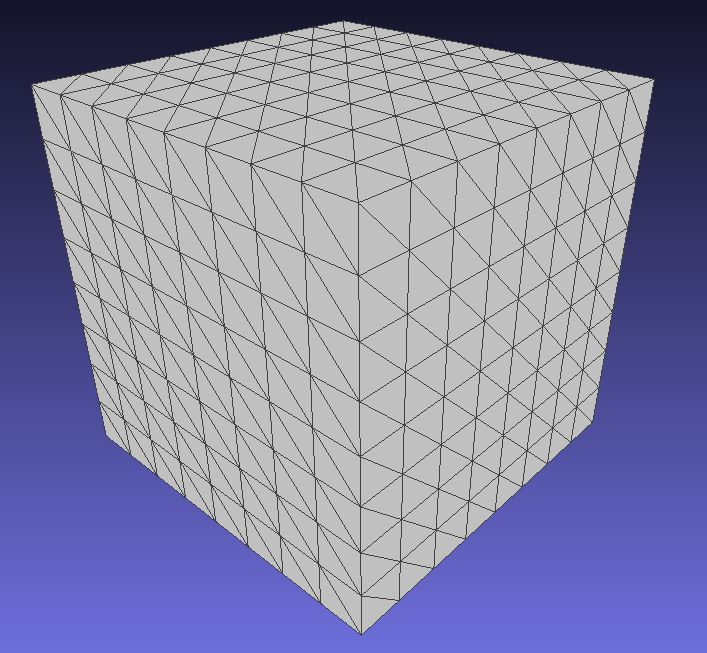
\includegraphics[width=0.35\textwidth, height=\textheight, keepaspectratio]{hr_cube_orga}
    \caption{cube made with organic modeling; a high number of mesh increases the resolution but complicates the modification of the volume shape.}
    \label{fig: hr_cube_orga}
\end{wrapfigure}

\paragraph{Organic modeling} is used to create natural geometries with rounded or irregular shapes, such as animals, plants, stones, humans and organs. The model consists of a surface made of polygonal faces, generally triangles, called \emph{mesh}. The density of polygons on the surface accounts for the resolution in the representation of details. Most of the models used in the medical field belong to this category, especially the models of parts of the human body. \\
The most common format for store organic models is the \textbf{.STL} (\emph{Stereolithography}, Standard Tasselation Language), which is a collection of triangular surfaces defined by the position of vertices in space and from the normals to the surfaces. The language was developed by 3D Systems for specific use with stereolithography machines, but it is now the standard language for models to be used with 3D printing. \\ A consortium of companies operating in the field of three-dimensional modeling and in additive manufacturing is currently at work for the creation of a new standard format, the \textbf{.3MF} (\emph{3D Manufacturing Format}) \parencite{Reference143}.

\begin{wrapfigure}{R}{0.35\textwidth}
% \ Centering
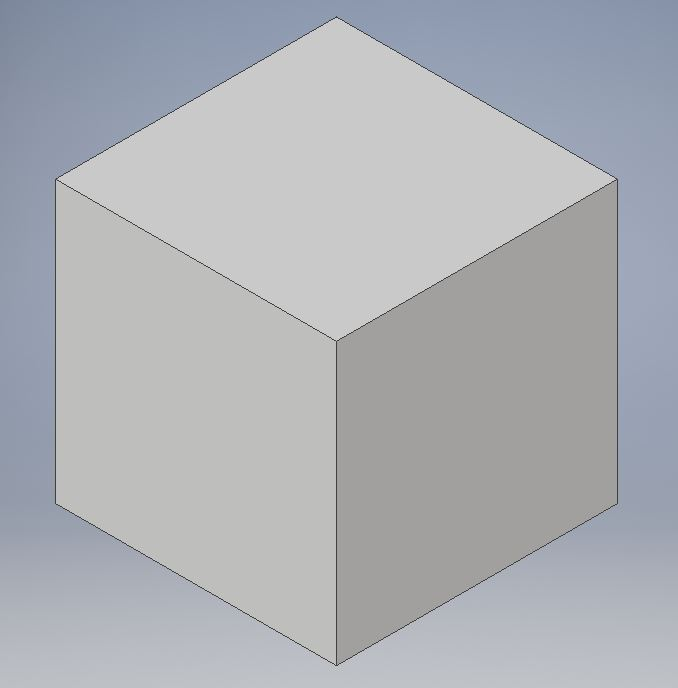
\includegraphics[width=0.35\textwidth, height=\textheight, keepaspectratio]{cube_geom}
    \caption {cube made with geometric modeling; the lowest number of faces is used to describe the cube.}
    \label {fig: cube_geom}
\end{wrapfigure}

\paragraph{Geometrical modeling} is used for the design of artificial parts, where the number of faces of the model must be optimized to simplify the design, the production and ensure the future adaptability of the design. The most widespread type of geometrical modeling is the \emph{parametric modeling}, adopted by major CAD software. Parametric modeling is based on the use of \emph{geometric primitives} (lines, curves \ldots) whose dimensions are defined and correlated. Parametric modeling is indicated for the design of engineering products, prosthesis and surgical guides. The output format of the model is dependent on the software used, but most parametric design software allows to export the models in .stl for the 3D printing procedures. The exported .stl model should be assessed for eventual conversion errors.

\section{3D Slicer}
3D Slicer is an open source software for the management and visualization of diagnostic images, made by developers and researchers in the medical field in a project supported by the \emph{National Institute of Health} (NIH), with the collaboration of companies such as \emph{Kitware Inc.} and \emph{General Electric}, and an expanding community of developers \parencite{Reference28}. \\
3D Slicer allows to manage DICOM files from \textbf{PACS} server (\emph{Picture Archiving and Communication System}) and non-specific archives, and allows to view and process images in 2D, 3D and 4D (X, Y, Z and T, \emph{time}, for example detection with ultrasound probes). The software offers the ability to render images and to create templates for use with CAD software \parencite{Reference31}.\\

From a software point of view, Slicer has a modular structure, with basic modules (\emph{Core modules}) that provide generic DICOM file management (\emph{DICOM}), rendering (\emph{Volume Rendering}) and the functions of image transformation in 3D space (\emph{Transforms}). Some of the other relevant modules are:
\begin{itemize}
\item \emph{\textbf{Filtering}}: contains tools for preparing the image for subsequent processing (\emph{preprocessing}). The most used features include arithmetic operations, noise reduction and correction of the density distribution of the scan, however there are dozens of other algorithms that can be used.
\item \emph{\textbf{Registration}}: provides the ability to align two scans with each other, useful when aligning different scans of the same patient, or orienting scans to standardize a dataset.
\item \emph{\textbf{Segmentation}}: segmentation is the separation of the image into smaller regions based on their characteristics. 3D Slicer integrates both interactive (with human input) and automatic segmentation methods.
\item \emph{\textbf{Surface models}}: allows the creation and management of surface volumes to be exported for further processing in other software.
\item \emph{\textbf{Image guided Therapy}}: gives the possibility to exchange data in real time with peripherals including robotic devices, scanners and radiotherapy devices.
This feature allows peripheral devices to be used in conjunction with diagnostic images, and may be of interest for use as \emph{virtual guide to implant placement} \parencite{Reference118}.
\end{itemize}

Other modules are present, and the collection is frequently expanded with modules created by the community, institutions and companies. Furthermore, each user can create a module and distribute it as a source or as a binary file (an executable file); this path can be used for packages that contain non-free proprietary code, but whose authors still want to distribute the functionality to the community \parencite{Reference28}. \\
The software is accompanied by publications and a documentation describing the implemented functionality \parencite{Reference28}, \parencite{Reference29}, \parencite{Reference30}. The documentation is the best reference for users who want to use the software and should be consulted to fully understand the operations performed by each module. There is also a forum on which is possible to communicate with 3d Slicer users and developers \parencite{Reference35}.

\section{Blender}
Blender \parencite{Reference32} is free and open-source software for computer graphics, maintained by the \emph{Blender Foundation} and a community of volunteer developers. It provides basic mesh creation and management, and advanced features such as animations, rendering and physical simulations. \\
Blender is a software that covers many aspects of computer graphics. It is accompanied by an extensive documentation of its features \parencite{Reference33}. The Blender community is important and has contributed to the maintenance of the software during its evolution, together with the Blender Foundation. The community is the place where to exchange ideas with experts and software users, where to find tutorials and workflow examples for all the features of Blender \parencite{Reference34}. \\
Blender is very useful for the post-processing of the models created in 3d Slicer. The software allows to modify the meshes of the model and to perform operations such as \emph{smoothing}, the modification of the size and resolution of the mesh and to use Boolean operations between two models (\emph{difference}, \emph{union} and \emph{intersection}). It also allows rendering to create high-quality images of the models.

\section{MeshLab}
MeshLab \parencite{Reference36} is free and open source software that allows advanced mesh processing, developed by students and researchers of the \emph{Faculty of Computer Science of the University of Pisa}. The software allows the import/export of a large number of format in which the models can be found and integrates tools for the inspection of the mesh and for its cleaning, algorithms for remeshing and creation of meshes from point clouds (optical scans, photogrammetry ...) and the management of the associated textures. \\
This software is useful for cleaning models, correcting problems with meshes, reducing the number of meshes and changing the shape and distribution of meshes on the model and comparing the models with each other.

\section{MeshMixer}
MeshMixer \parencite{Reference38} is not an open-source software, but it is a free software released by the company \emph{Autodesk}, which allows the visualization and processing of the meshes. MeshMixer is a software with many features, in some cases overlapping with software such as Blender and MeshLab, provided with a rich documentation \parencite{Reference39}. \\
This software provides an easy-to-use interface and excellent model manipulation and 3d printing preparation capabilities. MeshMixer simplifies the process of inspection and repair of the model, integrate analysis algorithms and tools for mesh processing. MeshMixer is a versatile tool that can be used in various step of the digital workflow. \\
When working with simple models, MeshMixer can speed up the preparation for printing, with tools that allow to perform Boolean operations, drill holes and repair defect of the mesh. The software facilitates the selection of areas of the model to be separated or in which to perform specific operations.

\section{FreeCAD}
FreeCAD \parencite{Reference40} is free and open-source parametric modeling software supported by a community of volunteer developers. The software allows to manage the production chain of an object. Integrate modules to perform the technical sketch and realize the 3D design from the sketch or by writing mathematical functions. Features modules for multi-part assembly and physical simulation, as well as various other applications such as robotics or boat design. \\
FreeCAD is useful for the realization of precise models, such as surgical guides and prostheses, but also parts created specifically for the 3D printer and allow to create objects of general utility such as supports and containers. It is a versatile software and a tool to known for anyone approaching 3D printing with the intention of creating functional and not merely aesthetic objects.\\
FreeCAD is supported by a frequently updated online documentation \parencite{Reference41}, and an ebook useful for understanding the basic functionality of the software, with practical examples aimed also at the 3D printing processing \parencite{Reference42}.

\section{Inventor}
Inventor \parencite{Reference43} is a professional CAD software developed by \emph{Autodesk}. It is among the most advanced parametric modeling software, and integrates all the functions of FreeCAD plus many others. The software is provided by Autodesk with a subscription plan, but for the students it is possible to download a 3-year trial version, very useful to have an approach with the software and to test its characteristics in depth. Inventor offers an easy approach to topology optimization via a dedicated module.

\section{nTopology Element}
nTopology \parencite{Reference139} is a commercial software for managing \emph{lattices} and \emph{scaffold}. It is a paid software but there is a free version that allows you to have an overview of the functions. The software facilitates the integration of 3D models and their conversion to scaffold.\\ It is possible to load physical simulations into nTopology, through which scaffolds can be obtained that will be optimized with respect to the loads that they will have to sustain. We will use the Free version of this scaffold generation software.

\section{Cura}
Cura \parencite{Reference44} is an open-source software for converting 3D models to g-code (slicing). The software is distributed by Ultimaker, a manufacturer of FDM 3D printers, and supported by a community of volunteer developers. Cura is supported by a documentation of the features \parencite{Reference45} and in-depth articles \parencite{Reference52}. \\
The software allows to perform slicing of the model and to adjust the printing options. Cura allows the adjustment of many parameters, including the printing temperature, layers height, filling geometry and its percentage. It also allows the automatic creation of various types of supports, and integrates the ability to work with more than one extruder in the same print, to make prints with more than one material.\\
Slicing is an important process in the printing workflow because it translates the digital model into a series of instructions. These are provided to the printer and result in a sequence of operations that it performs to give rise to a physical model, which aims to be the exact copy of the digital model.\\
Cura documentation describes the various printing parameters very well, so the main parameters will be briefly described here and the practical implications will be analyzed.

\subsection{Quality}
The \emph{\textbf{Quality}} menu contains parameters for adjusting the layer height and the width of the extruded line. Reducing the value of these items results in an increase in quality, because smaller details can be reconstructed. The choice of these parameters is not arbitrary, but is based on the characteristics of the printer.\\
The \emph{layer height} depends on the resolution of the extruder movement on the Z axis, which in turn depends on the steps/mm, based on movement mechanics and step interpolation (microstep). For example, a screw transmission with 8mm pitch, 1.8 degree/step stepper and 16x microstep, does a maximum 0.04mm step on the Z axis, which translates into a maximum resolution of 0.04mm on the Z axis, with the layer height to be set in multiples of 0.04 to have the maximum precision that this hardware is capable of. \\
Lower layer height allows you to reproduce smaller details and have a surface finish with a smoother appearance, but also increases the printing time, because you will need more layers to reproduce the model.\\
Setting the height of the first layer (\emph{Initial layer height}) with a higher value than the subsequent layers generally gives a better adhesion of the object to the print bed, because a more abundant flow of material in the first layer helps to compensate for a printing plane that is not perfectly horizontal. \\
The \emph{layer width} depends on the diameter of the \emph{nozzle} used, with smaller nozzles that increase the details reproduction, and large nozzles that reduce printing times; these are currently found in diameters ranging from 0.15 mm to over 1 mm. The layer width setting should be set to a value close to that of the nozzle diameters, maintaining a range of freedom to optimize the printing result. Setting a value slightly lower than the actual diameter can increase the print quality, but must be evaluated from time to time; moreover, a smaller width increases the printing time, because more lines will be used to make up the model. The value can be increased to compensate for any nozzle wear, but it is a temporary remedy and it is preferable to replace the worn nozzle with a new one.

\subsection{Shell}
The \emph{\textbf{Shell}} menu allows you to adjust the parameters of the model walls (shell). We can independently adjust the thickness of the model surfaces, roof and floor. A greater thickness will give a greater resistance to the model and a greater resistance to fluids leakage (\emph{leaking}) that can flow inside the model (\emph{microfluidic platform}). There are also various parameters regarding compensation for the expansion or shrinking of the print material and for fine-tuning the reproduction of the model surface.

\subsection{Infill}
The \emph{\textbf{infill}} is the filling of the model, the one that is inside the shell whose parameters we have explained before. The quantity of infill can be set in percentage, with 0\% indicating the absence of infill and 100\% indicating the complete filling of the volume of the object. There are several \emph{pattern} of infill, some fast as \emph{Lines} or \emph{Grid}, others slower but with better absorption of forces, such as \emph{Cubic subdivision}, while still others useful for printing deformable objects, such as \emph{Concentric} and \emph{Cross}. \\
The infill gives resistance to the object and acts as a support for the upper layers of the model. The percentage of infill must be adjusted according to the mechanical conditions in which the infill has to operate. A model that undergoes stress during use must have a high infill and a suitable geometry, while an aesthetic model can be made with little or no infill, in order to save material and speed up printing.\\
The infill menu contains several parameters that can be adjusted, among them the possibility to manually set the angle of some patterns (\emph{Infill Line Direction}). Manual adjustment of the infill line angle is a quick method in which the design of simple three-dimensional scaffolds can be performed \parencite{Reference138}.

\begin{figure}[h]
    \centering
    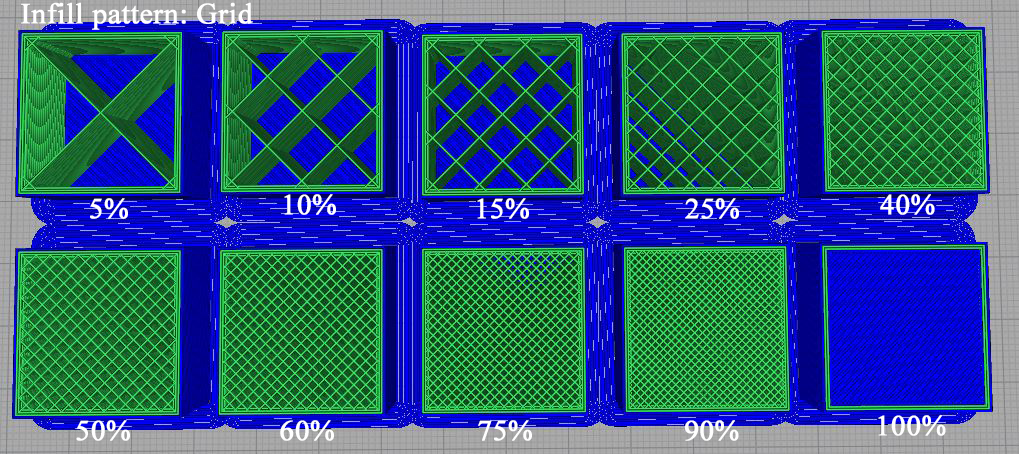
\includegraphics[width=\textwidth,height=\textheight,keepaspectratio]{numbers_grid_infillDens}
    \caption{\emph{\textbf{Infill pattern}}: \emph{Grid}; from left to right, progressive \emph{\textbf{Infill density}}.}
    \label{fig:numbers_grid_infillDens}
\end{figure}
	

\subsection{Material}
The \emph{\textbf{Material}} menu contains parameters for adjusting the temperatures and the extrusion process.
It is possible to adjust the \emph{printing temperature} and the temperature of the heated printing plate (\emph{build plate temperature}); you can set the temperature of the first layer independently of that of the subsequent layers. A higher temperature at the first layer favors the adhesion to the bed, because the extruded material is less viscous and flows better on the surface. The heated plate also facilitates adhesion, which is however related to the material of which the plate is made.\\
The \emph{flow} is regulated as a percentage and must be adjusted to avoid excesses or deficiencies of extruded material during printing. An adjustment method consists of observing the surface of the printed object to see if there are spaces or excesses between the layers, and varying the percentage of flow until it appears uniform. Another method is to print a cube without a roof, infill 0\% and with thick walls line (in \emph{shell} -> \emph{wall line count} = 1), and with a caliper measure whether the wall is actually thick the same value set in \emph{shell} -> \emph{wall line width}.
This empirical method can give an indication of the discrepancy between the actual width value and the real value. However, the relationship between the wall thickness and the flow value is not linear, because the extrusion quantity is influenced by parameters such as printing speed, actual filament diameter and printing temperature.\\
An important parameter is \emph{retraction}. Retraction is the distance that the filament is pulled back from the extruder each time a printed segment ends; this movement serves to reduce the pressure inside the nozzle and to limit the release of molten material during travels (\emph{oozing}). The values of retraction distance and retraction speed must be adjusted with appropriate tests, together with extrusion temperature and \emph{jerk}.

\subsection{Speed}
\begin{wrapfigure}{R}{0.4\textwidth}
\vspace{-20pt}
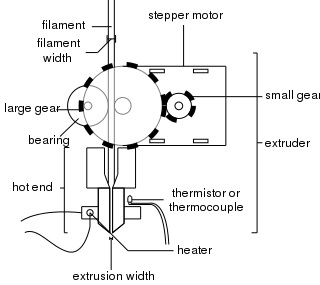
\includegraphics[width=0.4\textwidth, height=\textheight, keepaspectratio]{estrusore_diag}
    \caption{Direct extruder}
    \label{fig: estrusore_diag}
\end{wrapfigure}

The \emph{\textbf{Speed}} menu allows you to set the print speed. You can adjust the print speed of the shell and infill separately, the speed of travels and the accelerations during the various printing phases.
The \emph{jerk} is a parameter that manages the maximum instantaneous velocity change of the extruder; a low value smooths accelerations and decelerations while a high value makes them brusque. The effect of jerk is more evident when working at high speeds \parencite{Reference53}. \\
The printing speed must be adjusted according to the possibilities of the printer. Fast prints are generally less precise than slow prints, and for objects where accuracy is required a lower speed should be preferred. Fast prints cause vibration of the structure and instability in the flow of material, for which test prints must be made to evaluate how the printer behaves at various speeds.

\begin{wrapfigure} {R} {0.4\textwidth}
	%\centering
	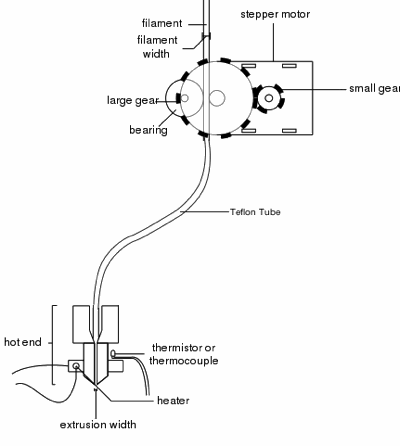
\includegraphics[width=0.4\textwidth, height=\textheight,keepaspectratio]{bowden}
    \caption{Bowden extruder}
    \label{fig:bowden}
\end{wrapfigure}

The speed also depends on the inertia of moving parts, so having a few light moving parts would help to increase speed in printing operations.\\
The filament extrusion system in FDM printers essentially consists of an extruder and an hotend. The extruder is the part that pushes the filament into the hotend, which warms up and melt the filament, which exit from the nozzle under the thrust of the extruder. On Cartesian FDM printers \emph{direct} extrusion is often used, which consists of the extruder connected to the hotend, both moving together on the axes.\\
To lighten the moving mass, and hence the inertia, it is possible to use an extrusion configuration called \emph{bowden} \parencite{Reference54}, \parencite{Reference55}, where the extruder is far from the hotend. The decrease in the moving mass, due to the dissociation between the extrusion process and the material melting process, allows printing at higher speeds without an excessive degradation of the printing quality. In the bowden extrusion the filament goes from the extruder to the hotend usually passing through a \emph{Teflon} (PTFE) tube, needing an obviously longer path than the direct extrusion; this makes the filament less responsive in the extrusion and retraction steps. This effect can be compensated for by adjusting the parameters of priming and retraction of the filament.

\subsection{Travel}
The \emph{\textbf{Travel}} menu contains options for managing printer movements during movements without extrusion. The \emph{Combing Mode} option restricts the movement of the nozzle to the print area of the model to reduce the need for retraction. This parameter can always be active, only active in the infill or off. To be adjusted according to the model to be printed, but pay attention to the fact that the nozzle moves on an already printed area and could damage it. Combing usually reduce printing time.
The \emph{Z-Hop} is a movement of the extruder on the Z axis at each retraction; by raising the extruder at the defined distance, it prevents the nozzle from touching the print during movements.

\subsection{Cooling}
The \emph{\textbf{Cooling}} menu provides tools for adjusting fan behavior during printing. During first layer printing the blower turned off favors good adhesion between the object and the printing plate; subsequently the fan speed can be increased up to 100\%. A good cooling of the material allows to print geometry with greater angles, using less supports for suspended areas (bridges). \\ Gradually increase the fan speed is preferable for the initial few layers, because it limits the deformation and detachment from the plane, especially with large prints. Some materials, such as \emph{nylon}, often require little or no cooling during printing, to prevent \emph{shrinkage} deformation.

\subsection{Support}
The menu \emph{\textbf{Support}} gives the possibility to create supports for the suspended or strongly inclined areas of the model. Various parameters can be adjusted on the quantity and shape of the supports, as well as the distance to be maintained by the object. During the creation of supports, a compromise must be sought between proximity to the object to be supported and ease in supports removal.

\begin{figure}[h]
	\centering
	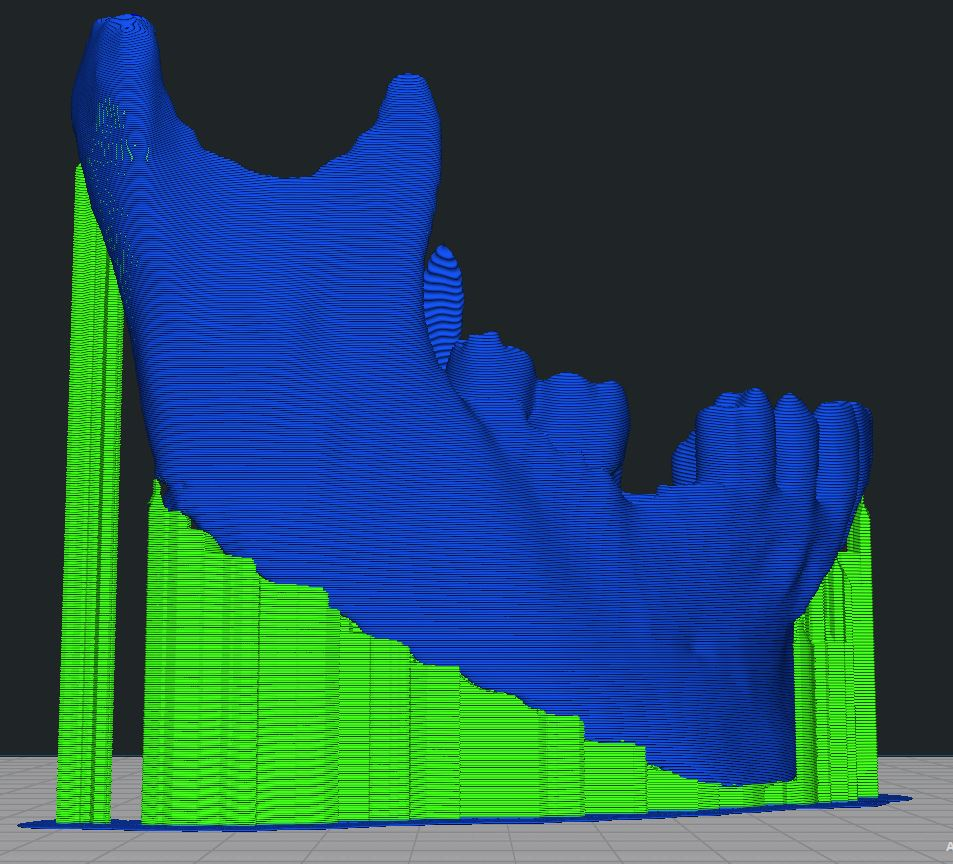
\includegraphics[width=0.5\textwidth, height=\textheight,keepaspectratio]{Supports}
    \caption{Supports in green}
    \label{fig:Supports}
\end{figure}

\newpage
	
\subsection{Build Plate Adhesion}
The \emph{\textbf{Build Plate Adhesion}} menu allows to generate contours or surfaces to facilitate the adhesion of the first layer to the plane.

\textbf{Skirt} is simply an extrusion turn made around the perimeter of the model to be printed, without touching it; it serves to prime the extruder, to extrude the material before printing so that the nozzle is ready to start the first layer.

\textbf{Brim} is a contour that joins to the edge of the first layer of the object. Its width can be adjusted and is an important help to keep the models sticking to the floor. It is also easy to remove and leaves virtually no marks on the model.

\textbf{Raft} is a few layers thick grid, produced between the printing plate and the object. Raft improves the adhesion even on an irregular surface and allows a good distribution of heat to the model. Useful for printing materials that deform greatly due to the printing process.

\begin{figure}[h]

\begin{subfigure}{0.3\textwidth}
\centering
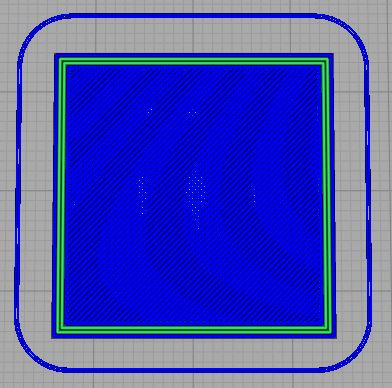
\includegraphics[width=0.6\linewidth, keepaspectratio]{skirt} 
\caption{Skirt}
\label{fig:skirt}
\end{subfigure}
\begin{subfigure}{0.3\textwidth}
\centering
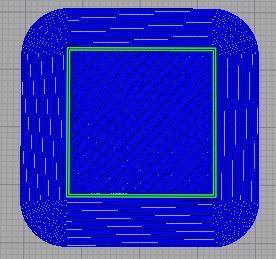
\includegraphics[width=0.6\linewidth, keepaspectratio]{brim}
\caption{Brim}
\label{fig:brim}
\end{subfigure}
\begin{subfigure}{0.3\textwidth}
\centering
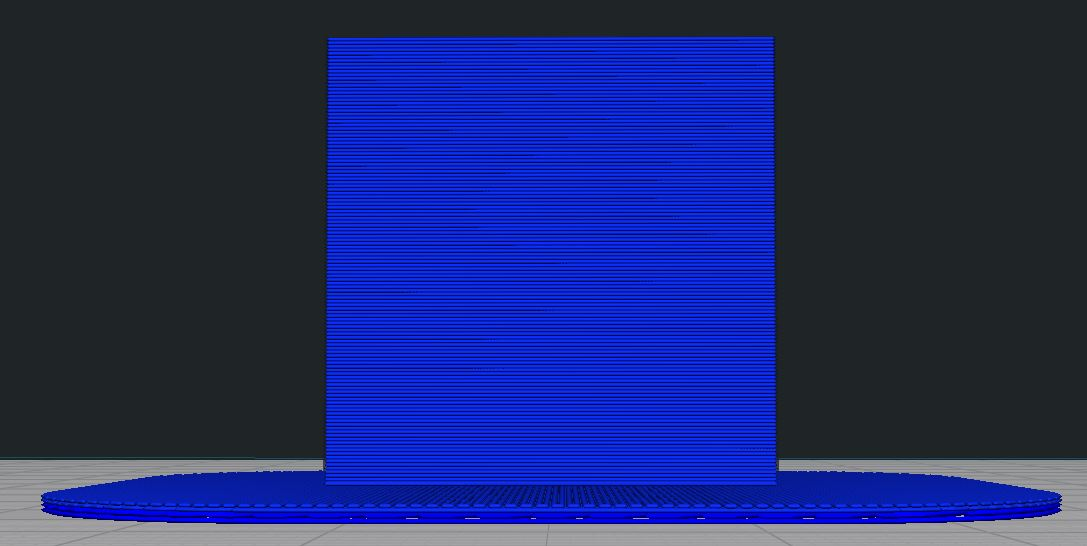
\includegraphics[width=0.8\linewidth, keepaspectratio]{raft}
\caption{Raft}
\label{fig:raft}
\end{subfigure}

\caption{\emph{Build Plate Adesion}.}
\label{fig:Build Plate Adesion}
\end{figure}
\vspace{-10pt}



\subsection{Fixes, Special Modes ed Experimental}
The other menus contain other advanced controls on the repair of the mesh during printing, special printing modes and experimental functions, which are not essential for the procedures here described, but which are still worth knowing, because they are useful in some situations.
In the \emph{\textbf{Special Modes}} we find the \emph{Print Sequence} option that gives the possibility to print objects on the plane all together or one at a time. \\
The \emph{Mold} option gives the possibility to create model negatives (a mold), which can be printed and used to recreate the original model by molding. \\
In \emph{\textbf{Experimental}}, the entry \emph{slicing tolerance} indicates how to slice the diagonal surfaces and affects the slicing mode \parencite{Reference56}. It is important to manage the tolerance of mechanical components that need adequate precision.

% Chapter Template

\chapter{3D Models from Medical Imaging} % Main chapter title

\label{Chapter4} % Change X to a consecutive number; for referencing this chapter elsewhere, use \ref{ChapterX}
 
 %----------------------------------------------------


We present a use case, which shows how to derive a 3D model from a series of diagnostic images. The procedure here described is used to give an overview of the main functionalities of the software and the basic techniques of images and model management with the aim of providing a generic workflow, and some insights useful for the optimal resolution of specific cases. \\
The case presented here shows how to get a model of the mandible and how to prepare it for printing. The presented procedure is well suited to the extraction of models of organs with a strong contrast to surrounding tissue, such as bone tissue in CT.

\section{Image anonymization}
Before starting to work with images we must ensure that these do not contain sensitive data with which we can trace the patient's identity. In this case we will use the open-source software \emph{DICOM Confidential}, developed by the team \emph{Data Intensive Research of the University of Edinburgh} \parencite{Reference46} \parencite{Reference146}. The software allows you to load a folder containing the images, which are then processed according to the defined directives. \\
When the software is opened, the graphical user interface (GUI) appears. Here is possible to upload the folder containing the set to be anonymized. \\
The entries \emph{Policy URI} and \emph{Workflow file} have to be filled. These are the indications on the workflow to be performed and on the anonymisation operations to be executed on the images. The software provides standard templates to be used. These can be modified as required, and are located in the path \path | C: Userpath \ DICOM Confidential | (where \path |C: Userpath \ DICOM Confidential | is the folder where the software was installed). \\
The output path is \path | C: Userpath \ DICOM Confidential \ data \ ANONYMISED |. Using the standard configuration files, each anonymized set will be recognized by the DICOM reading software (3D Slicer in our case) as belonging to the single patient "ANONYMISED", to which all the anonymized studies will be added. To be taken into account during the organization of the system.

\begin{figure}[h]
	\centering
	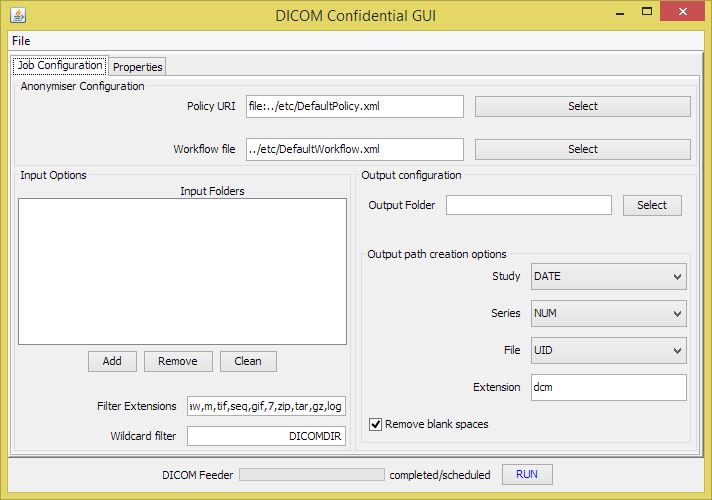
\includegraphics[width=0.9\textwidth, keepaspectratio]{gui_dicomConf}
    \caption{Schermata principale del software \emph{DICOM Confidential}}
    \label{fig:gui_dicomConf}
\end{figure}

\section{Anonymized Images}
Is possible to download anonymised datasets from \emph{The Cancer Imaging Archive} \parencite{Reference47}, a database maintained by the \emph{The National Cancer Institute} (NCI) and the \emph{University of Arkansas for Medical Sciences} (UAMS) to support multidisciplinary research, together with the \emph{Cancer Genome Atlas} dataset \parencite {Reference48} \parencite{Reference49}. \\
Several studies with various imaging techniques are available, which give the opportunity to deepen the analysis of various segments of the body and the oncological diseases that may occur.
To use the images, follow the simple procedures described on the website. Once the data is obtained, it can be loaded directly onto the visualization software.
                             
\section{How to use the dataset}
The images obtained can then be uploaded to 3D Slicer for viewing and processing. We will use a set of images downloaded from \emph{The Cancer Imaging Archive} portal, located within the \path | TCGA - HNSC collection, Subject ID: TGCA-BA-6868, scan: Neck BW Axial|. \\
The software uses the \emph{DICOM} module \parencite{Reference50} to load and manage diagnostic image sets. The \emph{Volume Rendering} module can be used to display a rendered image. \\
With the \emph{Crop Volume} module it is possible to cut the volume part of our interest (Region of Interest, ROI), to lighten the computer from data that are not needed at the moment; it will be very useful later when we work with the models. In this example we want to create a model of the \emph{\textbf{mandibular bone}}, so we orientate the ROI in a way that contains the maxillary bones, and apply the modification.

\begin{figure}[h]
\centering
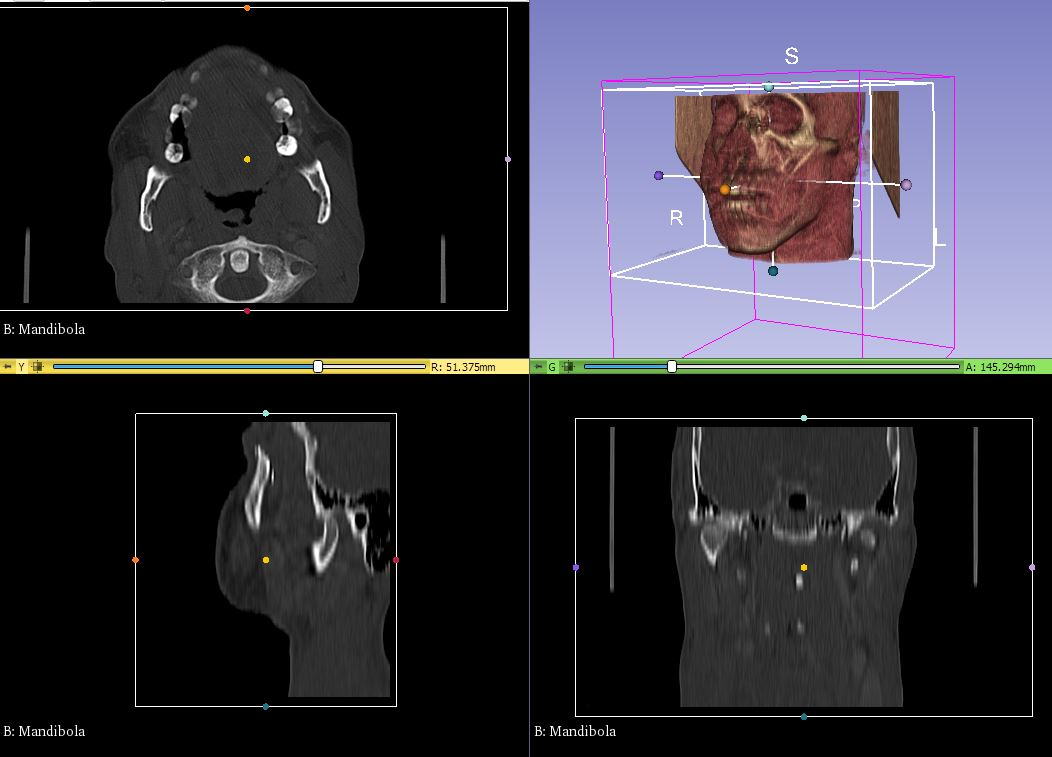
\includegraphics[width=0.8\textwidth, keepaspectratio]{crop1}
\caption{crop module used to select the upper and lower jaws region}
\label{fig:crop}
\end{figure}
\vspace{-10pt}
\section{Images Segmentation and Model Creation}

We can then start the segmentation, using the \emph{Segment Editor} module. This module contains several tools that allow us to highlight the areas of the images of our interest. Since we want to extract the model of a bone, the mandible, a quick method is to use the \emph{bone density range} to quickly highlight the region of our interest. Then with the \emph{Add} button we add a segment and select the \emph{Threshold} tool which allows us to select a density range to highlight. The \emph{Data Probe} tool at the bottom left gives us information about the point in the image where the mouse tip is located, and contains an entry indicating the density at the point.
Selecting the threshold we look for a compromise between completeness in capturing details and cleaning in the segmentation mask. We have the possibility to perform a manual finishing of the segmentation, so we can leave some unselected area from the threshold to have a greater cleaning between the parts to be segmented. We consider that the selected areas must be separated to be treated as different segment, except if a different segment is used for each area; in that case the selection voxels can be adjacent without merging the volumes into a single object.\\
However, it is important to select the areas of interest in the best way, and in the CT we are segmenting a delicate point for the correct jaw separation is in the area of the condyles, where the selection is continuous with that of the anterior wall of the glenoid cavity of the temporal bone. Another point that have to be separated is the posterior region of the dental arch, at the level of the occlusal plane, where the teeth of the jaw are probably joined to the antagonists.

\begin{figure}[h]
\centering
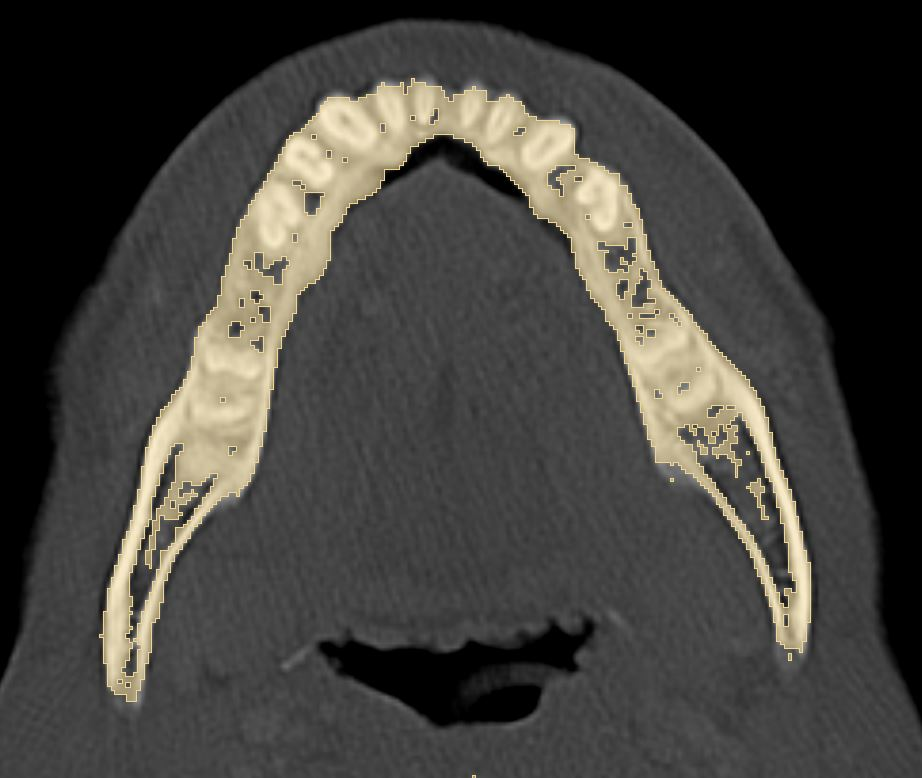
\includegraphics [width=0.6\textwidth, keepaspectratio]{origin_label}
\caption{Selection of mandibular bone and lower dental elements; \emph{threshold} 220 - 3071 HU; removal of small voxel groups: \emph{Island}> \emph{remove small island (minimum voxel=1000)}.}
\label{fig: origin_label}
\end{figure}

Once the threshold selection has been applied, we see that a mask has been created on the voxels that fall within the selected density range. This mask can be modified manually, adding any missing areas and separating the parts of our interest from the adjacent ones. By clicking on the button \emph{Show 3D} we can see the preview of the 3D model created by the segmentation; this option is useful to see if the selected areas correspond to the model we want to obtain, but when modifying the mask it is better to deactivate the option to save computational resources, and activate the 3D visualization only when necessary. \\
The removal of the contact areas between two selected region, in our case the mandibular condyle and temporal condyle, is performed in 3D Slicer to speed up the subsequent processing of the model. A model could have been created after the use of the threshold, but the separation of two models in software such as Blender is longer and more complex than the simple selection/deselection of voxels that can be performed in 3D Slicer.

\begin{figure}[h]
\centering
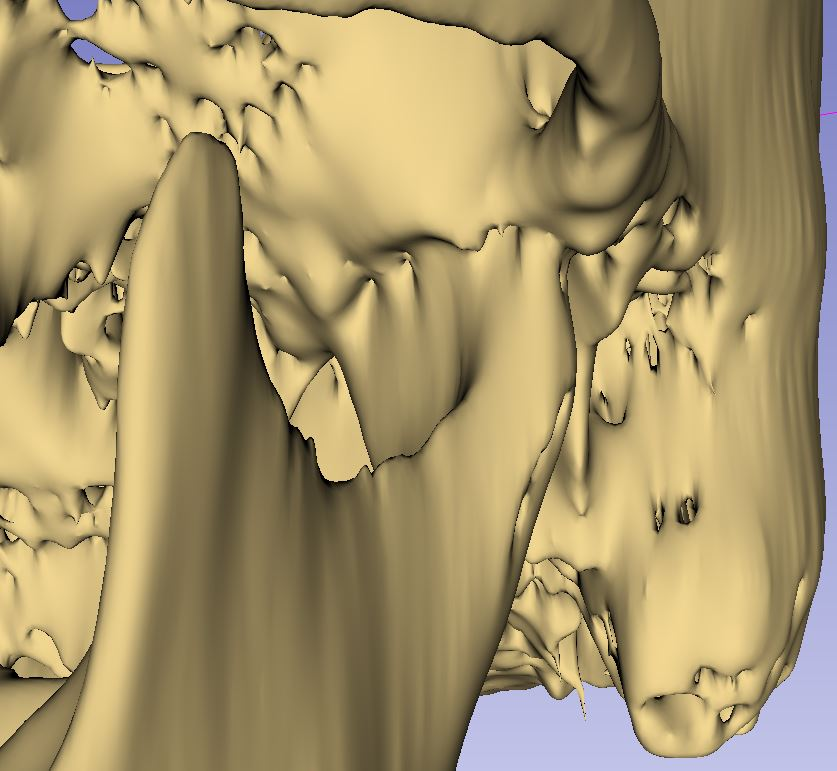
\includegraphics[width=0.4\textwidth, keepaspectratio]{fuso_condi}
\caption{3D reconstruction of the threshold segmentation of the mandible. The mandible is fused to the temporal bone.}
\label{fig:fuso_condi}
\end{figure}

We therefore aim to obtain from Slicer a 3D model as precise and clean as possible, to reduce the duration of subsequent steps, but also to create good quality segmentation datasets, which are useful for other purposes (data analysis, training set for Neural Network). \\
The \emph{Erase} tool allows to remove the voxels that do not need to be selected from the mask. \\
The \emph{Paint} tool allows the selection of voxels of interest that are not automatically selected by the threshold. \\
After finishing, we can use the \emph{Island} tool with the \emph{Keep Selected Island} option enabled; clicking on the jaw selection mask. If this island is separated from the rest of the selection we will have correctly performed the separation, which we can control by showing the model with the button \emph{Show 3D}. If we also want the model of the rest of the selection, we can click on the \emph{Undo} button to go back one step and retrieve the island containing the jaw and part of the skull.\\
We can create two separated segment: one for the mandible and one for the skull. We add a segment from the \emph{Add} button and we select it; using the \emph{Island} tool with the \emph{Add Selected Island} option we click on the skull mask and it will be added to the new segment. Separating objects into segments causes the spatial relationship between the parts to be lost, so if the parts need to be in a particular relation the \emph{Merge into single file} option must be selected to export the model as a single .stl file. It is then possible to separate this single model in its two components with the Blender software. \\
Then go to the module \emph{Segmentation}, where from the menu on the left we find the window \emph{Export to File}; select the destination folder and export the files in .stl format.

\vspace{-10pt}
\begin{figure}[h!]
\centering
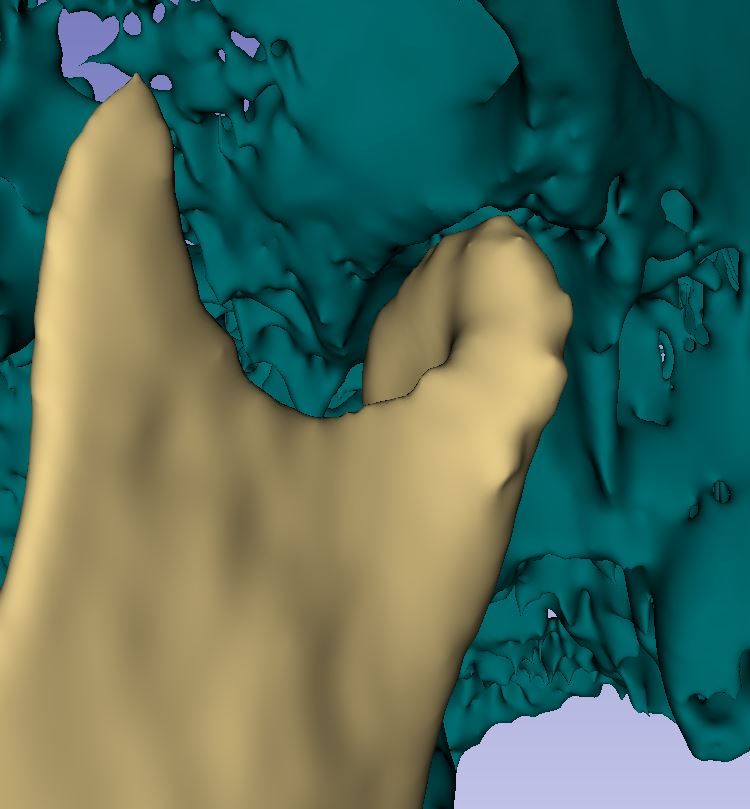
\includegraphics [width=0.4\textwidth, keepaspectratio]{sepa_condi}
\caption{Mandible separated from the temporal bone. The separation was done manually with the erase and paint tools. After separation a Segment for the jaw (yellow) and one for the skull (blue) were created.}
\label {fig: sepa_condi}
\end{figure}
\vspace{-15pt}

\newpage

\section{Model processing}
We import the model obtained in to MeshMixer and in the \emph{Analysis} menu we select the \emph{Inspector} tool. This function essentially has the task of detecting faults that must be resolved in order to have a closed model (\emph{manifold}) and to remove components separated from the main mesh. It is useful for preparing a model for 3D printing, where it is necessary that the model is precisely closed,  \emph{watertight}. This tool is useful for solving small problems with the mesh, but complex situations may require manual repair, which can be performed in this software as well as with Blender and MeshLab.

\begin{figure}[h]
\centering
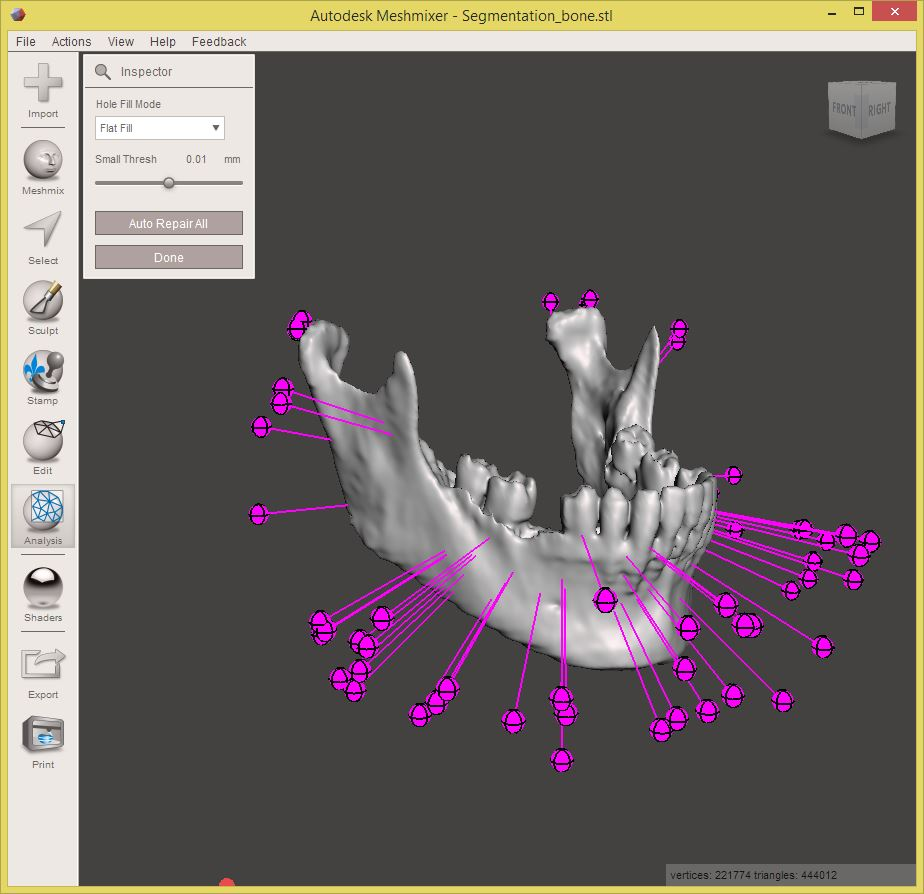
\includegraphics[width=0.8\textwidth, keepaspectratio]{inspector}
\caption{\emph{Inspector} tool in MeshMixer. Each violet indicator marks a fault in the mesh that can be fixed clicking on it.}
\label{fig:inspector}
\end{figure}

The model can then be exported to Blender to perform a smoothing. In Blender \emph{Modifiers} menu, select the \emph{Smooth} modifier. This is a function that smooths the surface of the object, causing a slight decrease in the object volume. In the instrument menu we can set the number of filter passages on the model; we find a compromise between smoothing and maintaining the original model dimensions. Another way to smooth the surface is to do it manually, with the sculpting tools \emph{sculpting} present in both Blender and MeshMixer. \\
After the model smoothing we inspect it to evaluate its quality; MeshLab can be used to compare two meshes. In our case we will measure the difference between the original model and the model obtained after 50 iterations of the \emph{smooth} modifier in Blender. When the models are aligned with each other, the procedure is to use the \emph{Hausdorff Distance} filter to evaluate the distance between the two meshes \parencite{Reference90}, \parencite{Reference91}. The software will return measurements related to the mesh sampling. \\

\begin{figure}[h]
\centering
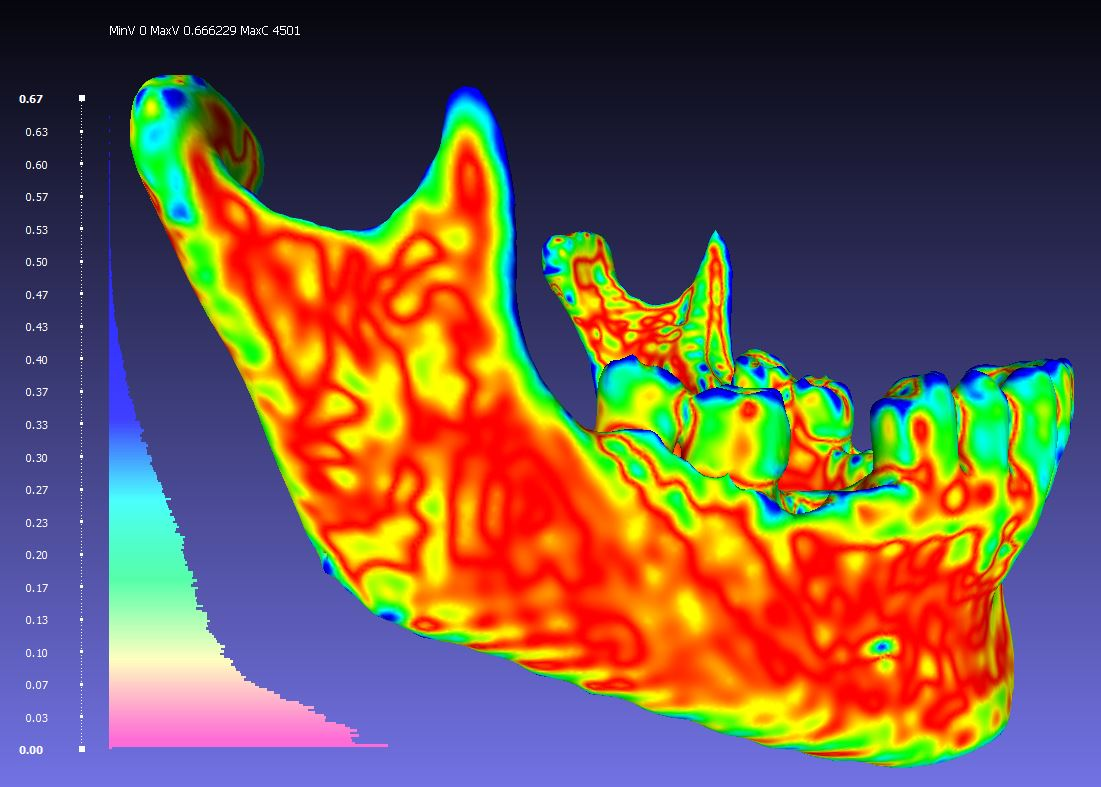
\includegraphics[width=0.8\textwidth, keepaspectratio]{hausdorff_smooth_clean}
\caption[LoF entry]{Hausdorff distance evaluation between the original model and the same model after 50 "Smooth" step in Blender. Legend goes from Red (no error) to Blue (max error).}

\begin{lstlisting}
Hausdorff Distance computed
Sampled 4657134 pts (rng: 0) on smooth_clean_Segmentation_bone.stl
searched closest on clean_Segmentation_bone.stl
min: 0.000000; max: 0.695190; mean: 0.116956; RMS: 0.154653

Values w.r.t. BBox Diag (181.472809)
min: 0.000000; max: 0.003831; mean: 0.000644; RMS: 0.000852 
Applied filter Hausdorff Distance in 29689 msec

Quality Range: 0.000000 0.666229; Used (0.006929 0.335713)
percentile (5.000000 95.000000) 
Applied filter Colorize by vertex Quality in 51 msec
\end{lstlisting}
\label{fig:hausdorff_smooth_clean}
\end{figure}

The mesh can then be colored to visually evaluate the discrepancy with the original mesh. To do this from the \emph{Filter} menu, select \emph{Color Creation and Processing} -> \emph{Colorize by Vertex Quality}. We can render the histogram from the menu \emph{Render} -> \emph{Show Quality Histogram}. \\
Keep in mind that the color scale goes from red to blue, where the \emph{red} indicates maximum correspondence with the original mesh, while the \emph{blue} indicates greater distance from the original mesh. The value is shown in model units, in this case millimeters. \\
As an alternative to MeshMixer it is possible to use MeshLab to perform more advanced mesh operations.
To remove regions separated from the main mesh, use the \emph{Filter} -> \emph{Cleaning and Repairing} -> \emph{Remove Isolated Pieces} tool, setting the minimum number of faces at a fairly high level, based on the number of faces shown in the bottom tool-bar. \\
To obtain a \emph{2-manifold mesh} \parencite{Reference92}, \parencite{Reference93}, in practical terms a \emph{closed mesh}: from the menu \emph{Filter} -> \emph{Cleaning and Repairing } use the functions: \emph{Remove Duplicate Faces}, \emph{Remove Duplicate Vertex}, \emph{Remove Unreferenced Vertices}, \emph{Remove Faces From Non Manifold Mesh}, \emph{Remove t-vertices From Non Manifold Edges}. \\ These commands clean up the mesh; to rebuild the 2-manifold mesh we use the command \emph{Filter} -> \emph{Remeshing, Simplification and Reconstruction} -> \emph{Screened Poisson Surface Sampling} \parencite{Reference95}, \parencite{Reference96}. This clean, 2-manifold reconstruction can be used for further processing. By performing an assessment of the quality of the reconstruction, it is noted that the agreement with the original mesh is very high.

\begin{figure}[h]
\centering
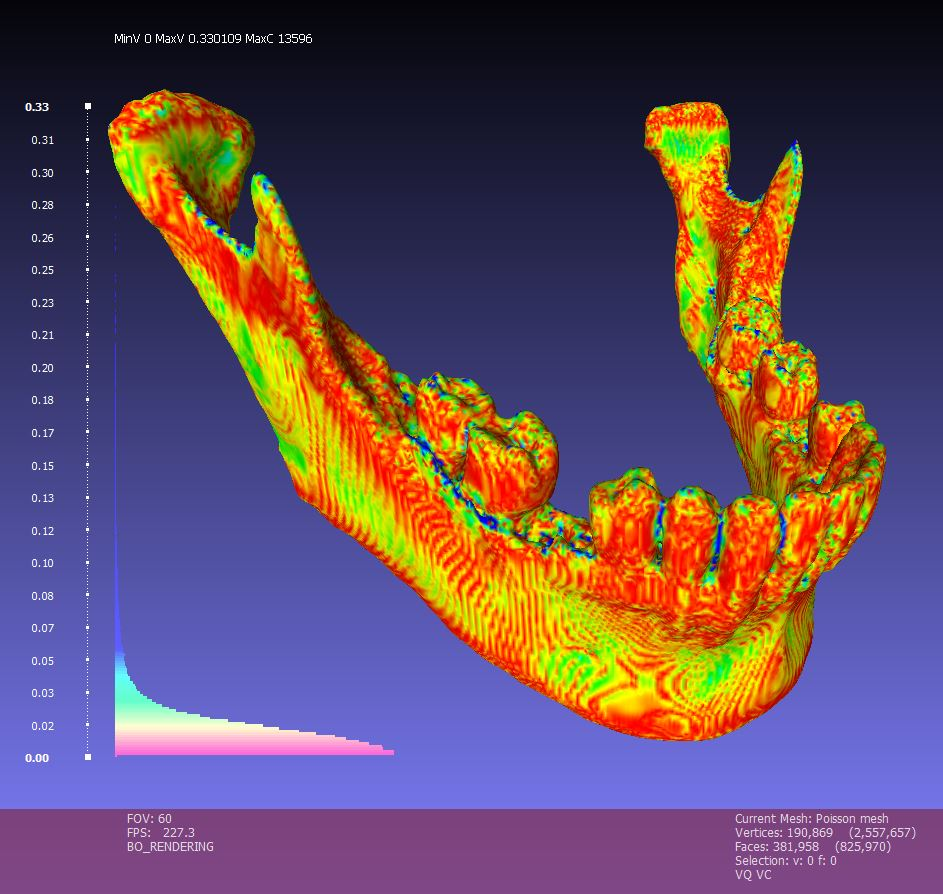
\includegraphics[width=0.75\textwidth, keepaspectratio]{noSeparate_poisson_clean_hausdorff}
\caption[LoF entry]{Hausdorff distance assessment after \emph{Screened Poisson Surface Sampling} algorithm.}

\begin{lstlisting}
Hausdorff Distance computed
Sampled 4195438 pts (rng: 0) on Poisson mesh searched 
closest on Segmentation_bone.stl
min : 0.000000 max 0.432402 mean : 0.019149 RMS : 0.031849

Values w.r.t. BBox Diag (182.226028)
min : 0.000000 max 0.002373 mean : 0.000105 RMS : 0.000175 
Applied filter Hausdorff Distance in 20254 msec
\end{lstlisting}
\label{fig:noSeparate_poisson_clean_hausdorff}
\end{figure}

We can make additional checks with the MeshMixer \emph{Inspector} tool to assess the need for further mesh refinements.
The model must then be exported in .stl format to prepare it for 3D printing.

\section{Slicing}
The digital model of the Jaw was obtained from the TC and processed to ensure a model suitable for printing. We will be slicing the model using the Cura software.\\
Load the model and select the \emph{Print Setup} > \emph{Custom} entry, to have the ability to fine-tune the printing parameters, which are initially hidden and must be activated. \\
The settings to be adjusted depend on several variables, including:

\begin{itemize}
\item the characteristics of the printer;
\item the characteristics of the model to be printed;
\item the printing material;
\item the accuracy and the mechanical properties expected from the object that we approach to print.
\end{itemize}

The environmental conditions in which you work are also to be taken into account, because for example some parameters may change between a print executed in a closed printer or in an open one.
The calibration of the printer and the knowledge of its specifications are fundamental for good printing result. Cura will generate printing instructions for the printer based on the printer specifications we entered in the \emph{Printers} > \emph{Machine Settings} menu. These settings are often updated with the addition of the most popular printer data, but for self-assembled printers the parameters must be entered manually. \\
With the calibrated printer and the information correctly entered in Cura, the model will be displayed in the software and will be sliced with the parameters entered. Once the slicing procedure has been completed we will be able to see the model layer by layer (\emph{Layer View}).
The so obtained \emph{\textbf{G-code}} can be used by the printer to produce the model.

\begin{figure}[t]
\centering
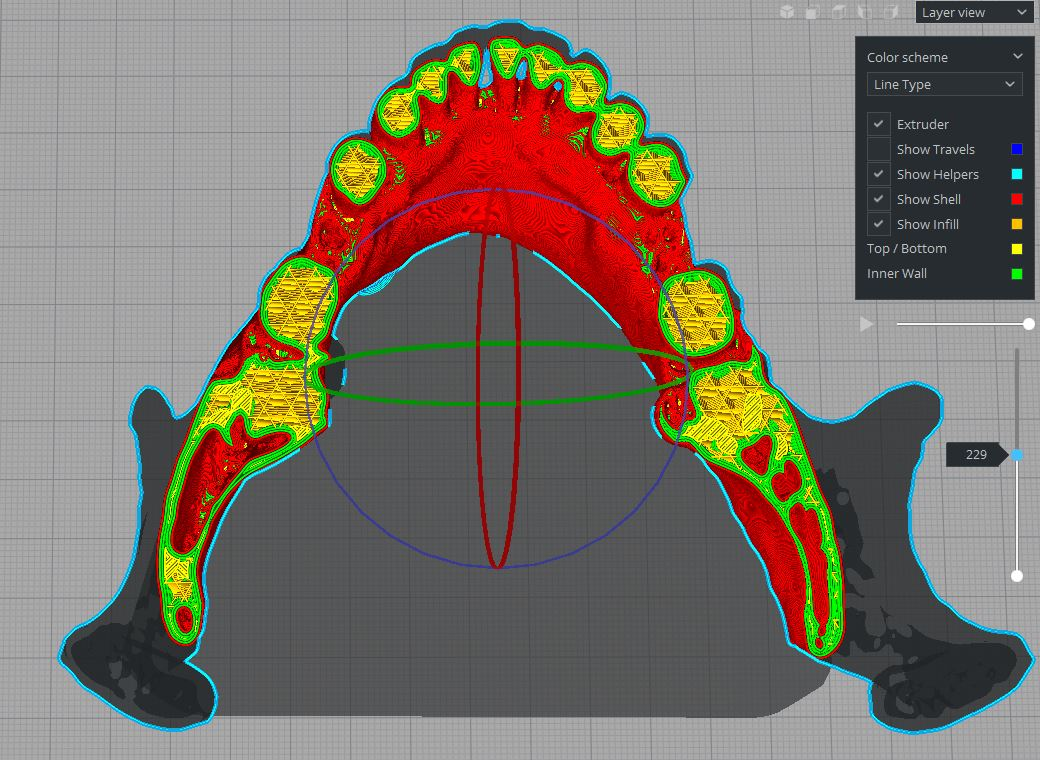
\includegraphics[width=\textwidth, keepaspectratio]{slicing}
\caption{Slicing of the mandible model in Cura.}
\label{fig:slicing}
\end{figure}

 
% Chapter Template

\chapter{3D Printing Process} % Main chapter title

\label{Chapter5} % Change X to a consecutive number; for referencing this chapter elsewhere, use \ref{ChapterX}

 %----------------------------------------------------

3D printing, also called \emph{rapid prototyping} or \emph{additive manufacturing}, is a manufacturing technique that allows to obtain physical objects from digital models, through the creation of two-dimensional sections of the object to be manufactured, which are produced one on top of the other to form the final three-dimensional prototype.

\section{Additive Manufacturing Technologies}
Various printing techniques and many materials are available such as thermoplastic polymers, gypsum, paper, light-curing resins, metals, ceramics, gels and others \parencite{Reference119}, \parencite{Reference120}. Each rapid prototyping technique has special characteristics that adapt to the solution of specific problems. Therefore we will describe the main additive manufacturing techniques used in the dental field, and then we will see their clinical implementation.

\subsection{Fused Deposition Modeling (FDM)}

\begin{wrapfigure} {R} {0.4\textwidth}
\vspace{-40pt}
	\begin{center}
	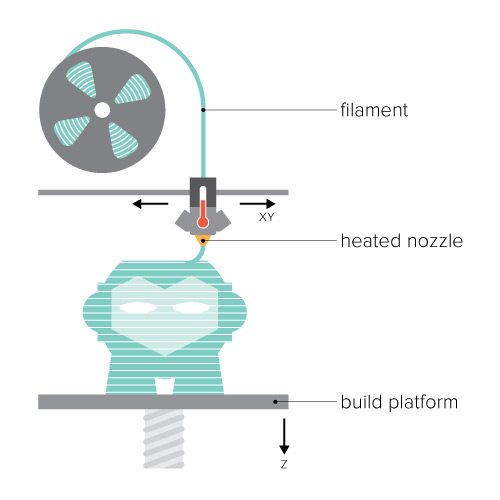
\includegraphics[width=0.4\textwidth, height=\textheight,keepaspectratio]{fdm_3d}
    \caption{FDM printing process}
    \label{fig:fdm_3d}
	\end{center}
\vspace{-40pt}
\end{wrapfigure}

FDM printing, also known as \emph{Fused Filament Fabrication} (FFF), consists of the deposition of a thermoplastic polymer, which is extruded through a thermostatically controlled nozzle on a plane, layer by layer until the production of the three-dimensional model. This type of technology adapts to various low viscosity materials and thermoplastic materials, is inexpensive and relatively fast. The accuracy depends on the specifications of the printer, up to few tens of microns.
\pagebreak

\subsection{Stereolithography (SLA)}

\begin{wrapfigure} {R} {0.37\textwidth}
\vspace{-40pt}
	\begin{center}
	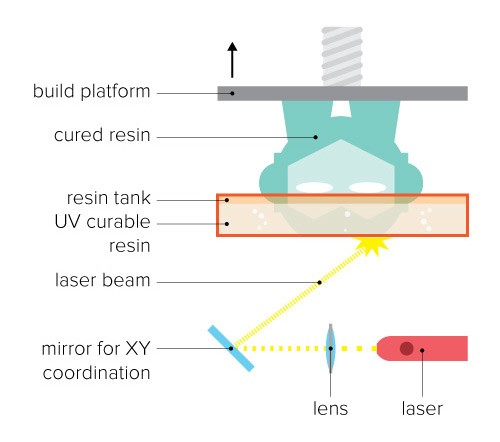
\includegraphics[width=0.37\textwidth, height=\textheight,keepaspectratio]{sla_3d}
    \caption{SLA printing process}
    \label{fig:sla_3d}
    \end{center}
\vspace{-40pt}
\end{wrapfigure}

Stereolithography was the first additive manufacturing technique to be patented in 1984 by \emph{Chuck Hull} \parencite{Reference124}. This technology uses a laser beam to locally polymerize resin following a computer defined 2D path, layer by layer until the designed 3D model is obtained. This type of printing is very precise and allows to print various types of resins with different properties. In the dental field there are calcinable resins, resins for prostheses, for temporary restorations, for surgical guides and other uses.

\subsection{Digital Light Processing (DLP)}

\begin{wrapfigure} {R} {0.37\textwidth}
\vspace{-40pt}
	\begin{center}
	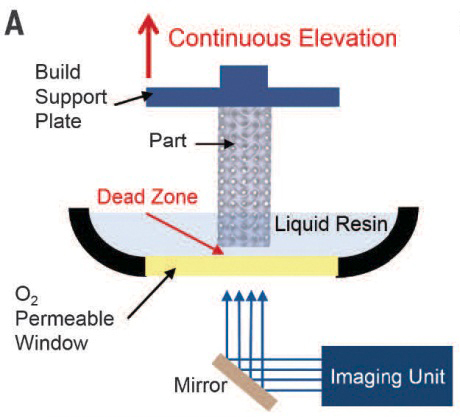
\includegraphics[width=0.37\textwidth, height=\textheight,keepaspectratio]{clip}
    \caption{CLIP printing process}
    \label{fig:clip}
    \end{center}
\vspace{-20pt}
\end{wrapfigure}

DLP printing also uses resin polymerization layer by layer, but instead of a laser such as SLA, it uses \emph{Digital Micromirror Device} (DMD, the same technology as projectors) to create a polymerization mask that polymerizes the entire layer at once. This technique is very fast in objects production. The print resolution depends on the resolution of the projected light beam, but in general it is very close to that of SLA. A recent evolution of DLP printing is the CLIP \parencite{Reference121}, \parencite{Reference122}, which allows very fast production of high-resolution structures. The CLIP technology was developed by the company Carbon Inc. \parencite{Reference123}.

\subsection{Selective Laser Sintering (SLS)}

\begin{wrapfigure} {R} {0.40\textwidth}
\vspace{-30pt}
	\begin{center}
	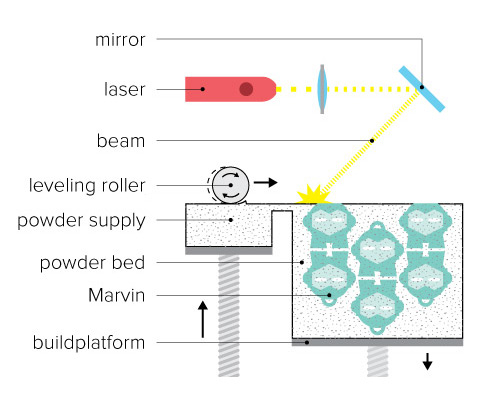
\includegraphics[width=0.40\textwidth, height=\textheight,keepaspectratio]{sls-technology}
    \caption{Processo di stampa SLS}
    \label{fig:sls-technology}
    \end{center}
\vspace{-40pt}
\end{wrapfigure}

SLS printers use a high power laser to sinter particles of polymers, metals and ceramics. The resolution is in the order of few tens of micrometers. This technology finds various applications in the dental field, because it allows both to print polymers, for surgical guides and models, and to print ceramics and metals, with immediate possibilities to use it in the prosthetic, implantology and surgical fields.
\newpage

\subsection{Material jetting (InkJet - PolyJet)}

\begin{wrapfigure} {R} {0.5\textwidth}
\vspace{-20pt}
	\begin{center}
	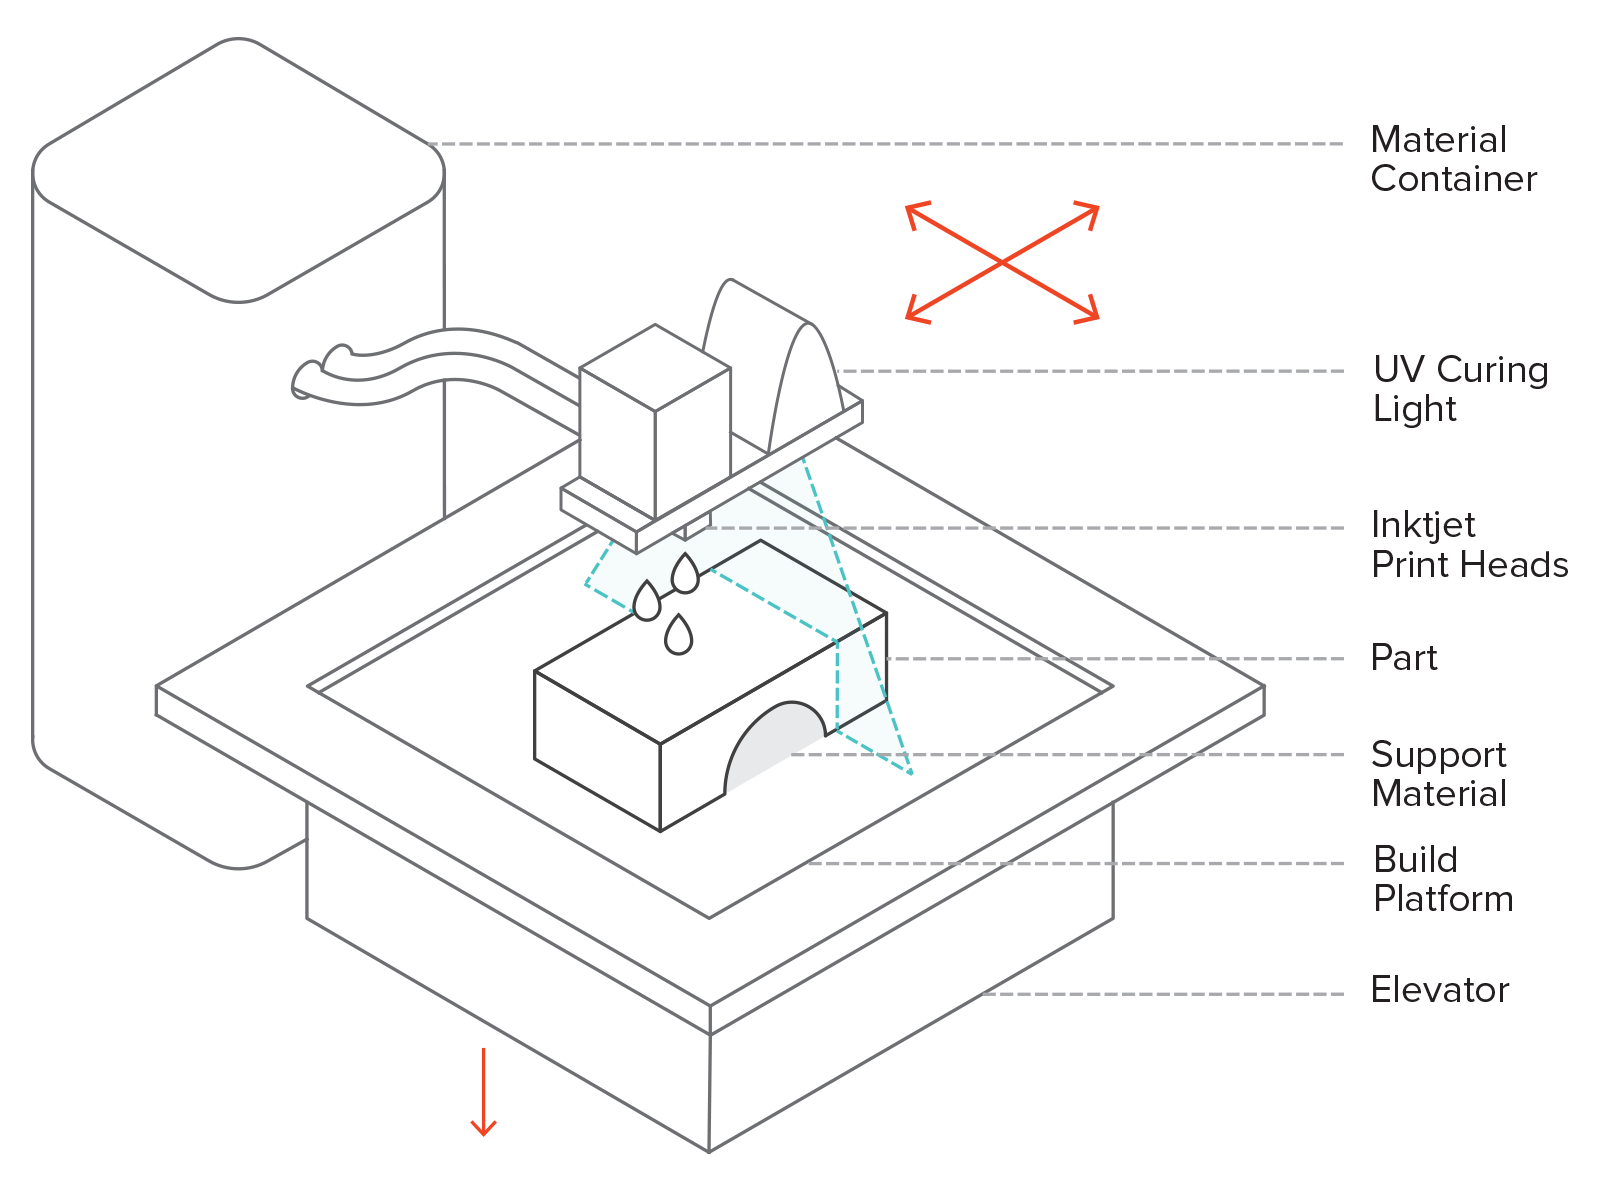
\includegraphics[width=0.5\textwidth, height=\textheight,keepaspectratio]{3-mj-schematic}
    \caption{\emph{Material Jetting} printing process}
    \label{fig:3-mj-schematic}
    \end{center}
\vspace{-20pt}
\end{wrapfigure}

The Material-jet printer uses a printing head that moves on the printing surface depositing the material, which is then light-cured by a UV light, in a process very similar to ink-jet 2D printing. \\
There are many materials that can be printed simultaneously; this makes it possible to print objects with non-uniform mechanical characteristics, where for example there are both rigid and elastic areas in a single structure. In addition, printing multiple materials at the same time allows to print objects with a wide variety of colors. Printing is also very precise, because the layer of material deposited at each passage is very thin (in the order of \SI{20}{\micro\metre}).

\section{Start the printing process}
The Fused Deposition Modeling printing process on a Cartesian printer is discussed here. \\
After obtaining the file in G-code from the slicing software, this file can be sent to the printer for printing. Depending on the capabilities offered by the printer's electronic control board, the G-code can be submitted to the printer in various ways.

\subsection{Printing via USB}
It consists of connecting the printer motherboard to the PC via a USB cable.
It has the advantage of being a fast method and allows the control of the printer from the graphic interface of the software installed on the PC \parencite{Reference2}. \\
A big disadvantage is the fact that the PC must necessarily be turned on throughout the printing process, and that any system crashes can stop printing suddenly and with little chance of recovery.

\subsection{Printing via SD Card}
Most of the motherboards for 3D printers currently on the market allow you to insert a microSD card, from which you can print the G-code files previously loaded on the card. \\
Printing from SD is very advantageous because it does not require the use of a PC during printing.
Many motherboards also allow you to load the G-code file on the microSD without removing it from the printer, simply by connecting the motherboard to the PC via USB to perform the transfer of the G-code on the microSD.
Printing from a memory card thus makes it possible to have a stand-alone 3D printer, which reduces the risk of printing failure due to problems that may occur to the PC during that phase.

\subsection{Printing via Web Interface}
More advanced motherboards, such as open-source \emph{Duet3D} \parencite{Reference3}, have the ability to connect to the Internet and allow printer control through the browser. This type of control greatly increases the flexibility of the printer, which can also be monitored while you are away from the printing place.\\
The web interface allows the user to remotely control even more than one printer, provided that these are equipped with control board with web connectivity. This is extremely useful when multiple printers must be managed and monitored at the same time, as can happen in the educational field or in the industrial sector. Remote monitoring can also be performed by connecting a video camera to this card, which allows real-time video monitoring, saving the videos for later analysis or for the next projection for educational purposes. \\
OctoPi is an open source operative system (OS) basen on Raspbian that can be used in small controlling board as the Raspberry Pi \parencite{Reference148}. OctoPi enable an high level of control of the printer, with video monitoring capabilities and web interface. It is compatible with almost every printer regardless of the control board used.

\section{Calibration}
The calibration process varies depending on the printer model. The most advanced printers perform the calibration in an automated way, and require only a few checks by the operator. Cheaper or do-it-yourself printers could instead need several steps where operator intervention is required. \\
The calibration must certainly be done before the first use, in order to have a reliable, precise and consistent printer. The process \parencite{Reference4} consists of calibrating:

\begin{itemize}
\item Step/mm on the X, Y, Z and E axes (E = extruder)
\item Print bed leveling
\end{itemize}

\subsection{Step/millimeter}
To calibrate the steps/mm on the axes, you need to know some parameters of the printer components:

\begin{itemize}
\item \emph{\textbf{Angle per step}}: is the rotation that makes the axis for each step, measured in degrees. Generally corresponding to 1.8 degree/step (equal to 200 step/revolution) or 0.9/step (equal to 400 step/revolution). It is dependent on the stepper motor used.
\item \emph{\textbf{Microstep}}: it depends on the interpolation capacity of the motherboard's stepper drivers that control the stepper motor \parencite{Reference5}, \parencite{Reference6}. The microstep consists in sending low power pulses to the motor, to make it perform fractions of steps. This theoretically increases the print resolution, but as the interpolation increases, the torque decreases, so the motor may not have enough energy to perform the movement. This means that the fraction of rotation will not be performed until the number of pulses necessary to give sufficient torque to the motion is accumulated.\\ To note, from StackExchange answer of the user cmm \parencite{Reference149} on ref. \parencite{Reference6}:

\begin{displayquote}
A stepper motor torque-vs-position-error curve is like a sin curve.  There is zero torque at zero displacement, and maximum torque at one full-step displacement. This doesn't change with micro-stepping. Thus, if you are taking 1/128th of a full step, it will truly give you very little torque.  OTOH (On The Other Hand) if you happen to stop, given a full step, at 1/128th of a step in error, you will also have a very small torque toward the correct position.
\end{displayquote}

At the end of the story, high microstepping gives a smoother movement to the stepper given the higher movement resolution, and it need exact the same torque per angle as a low microstepping \parencite{Reference150}. At high microstepping the temperature of the stepper driver have to be assessed, especially if the electric current flowing through the stepper is high \parencite{Reference151}.

\item For axes with belt drive and pulleys (generally X and Y):

\begin{itemize}
\item Belt pitch in mm
\item Number of teeth of the pulley
\item steps / mm = (step / rev * microstep) / (belt pitch in mm * number of teeth of the pulley)
\end{itemize}

\item For axes with leadscrew transmission (generally Z) \parencite{Reference51}:

\begin{itemize}
\item Screw pitch in mm
\item steps / mm = (step / rev * microstep) / screw pitch
\end{itemize}

\item For the extruder:

\begin {itemize}
\item step / mm = (step / rev * microstep) * / (diameter of the extrusion gear * pi)
\item With reduction (\emph{wade extruder}): step / mm = (step / rev * microstep) * (n large pulley teeth / small pulley teeth) / (extrusion gear diameter * pi)
\end{itemize}

\end{itemize}

\subsection{Leveling of the print bed}
Adjusting the printing bed should be as horizontal as possible to have an optimal surface on which to deposit the printing material. The printing bed must be orthogonal to the Z-axis and parallel to the X and Y axes. This arrangement allows to have an optimal deposition of the first layer, which is fundamental to guarantee the correct geometry of the printed object, as well as favoring its adhesion to the bed. \\
The bed level can be adjusted manually, adjusting the height through screws, or in an automated manner. Automated leveling (\emph{Auto Bed Leveling}) is performed with the aid of one or more sensors that allow the printer to define the printing bed position in the space. Any inclination of the bed is then compensated by the motion of the extruder on the Z axis \parencite{Reference7}, \parencite{Reference8}. The bed leveling must be carried out with the extruder and printing bed at the working temperature to take into account the deformation of the components at high temperatures. \\
The auto bed leveling is performed with the G29 command. At the end of the bed probing, the machine reports a matrix with the data relating to the operation just carried out. This data can be used to get a better understanding of the bed's inclination, and help us adjust the bed and choose the best area to print a model.
Data can be plotted thanks to scripts on websites \parencite{Reference9}. The Duet3D card also allows the display of the printing bed \emph{heatmap} directly from the web interface \parencite{Reference10}.

\section{Print}
At the end of the printer's heating and leveling procedures, printing process begins. The use of brim is recommended to prime the extruder and to increase the adhesion of the object to the bed.\\
To obtain a fine adjustment of the first layer there are some firmware (Marlin, RepRap firmware) that offer the \emph{BabyStep} option (in Marlin \emph{Babystepping}); it gives the possibility, during printing, to send real time axes position adjustments. The Babystep is very useful during first layer printing, because it gives us the possibility to precisely adjust the position of the nozzle with respect to the printing bed, facilitating the creation of a uniform and well spread first layer. After any adjustment with Babystep has been carried out, printing continues until the end.

% Chapter Template

\chapter{Utilizzi del modello 3d in Odontoiatria} % Main chapter title

\label{Chapter6} % Change X to a consecutive number; for referencing this chapter elsewhere, use \ref{ChapterX}

 %----------------------------------------------------
 
 
Abbiamo discusso di come ottenere un modello 3d digitale dalle immagini diagnostiche e di come convertirlo in un modello fisico per mezzo della stampa 3D. Sia il modello digitale che il modello fisico sono elementi che possono elevare la qualità delle terapie fornite dal medico, ed allo stesso tempo sono di grande valore per il clinico ricercatore per la quantità di dati ottenibili.\\
I campi di applicazione sono molti ed abbracciano le discipline chirurgiche, l'educazione, procedure odontoiatriche quali l'implantologia, la protesi e la conservativa \parencite{Reference103}.
Discuteremo qui alcune delle implementazioni più rilevanti delle procedure che abbiamo descritto.

\section{Educazione}
\begin{wrapfigure} {R} {0.4\textwidth}
\vspace{-20pt}
	\begin{center}
	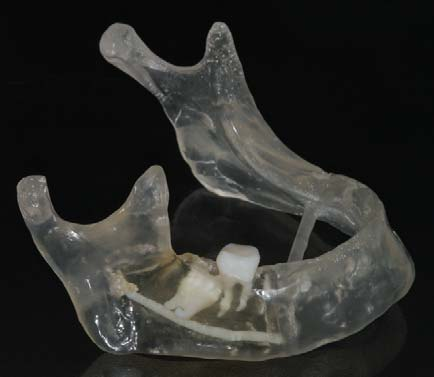
\includegraphics[width=0.4\textwidth, height=\textheight,keepaspectratio]{mandi_molar}
    \caption{modello3D ottenuto da CBCT, che presenta un terzo molare vicino al scondo molare, e con le radici in prossimità del nervo alveolare inferiore. Da \emph{Lambrecht et al} \parencite{Reference69}}
    \label{fig:mandi_molar}
    \end{center}
\vspace{-20pt}
\end{wrapfigure}
Nei corsi di laurea di ambito medico ed odontoiatrico il percorso di formazione del futuro professionista è un connubio di lezioni teoriche ed attività pratiche, volto a fornire delle approfondite conoscenze mediche ed un metodo di ragionamento clinico. Lo studente si trova soprattutto a dover sviluppare delle capacità manuali per eseguire degli interventi sul paziente.\\ Inoltre ogni studente in ambito sanitario studia l'\emph{anatomia}, e se un tempo le dissezioni su cadavere erano ciò che forniva agli studenti un contesto in cui applicare ciò che avevano appreso sui libri, ora sempre meno istituti offrono questa possibilità \parencite{Reference67}.\\
Con la diminuzione dell'uso dei cadaveri è aumentato l'utilizzo di repliche in plastica di parti dell'organismo come complemento pratico all'apprendimento dell'anatomia. Diversi autori hanno recentemente iniziato ad esplorare le possibilità offerte dalle moderne tecniche modellazione medica e stampa 3d nell'ambito della formazione medica.\\ Sono stati prodotti modelli anatomici e modelli per la spiegazione di procedure operative sia in ambito medico che odontoiatrico \parencite{Reference66}, \parencite{Reference70}. Heng \parencite{Reference67} ha valutato il miglioramento a breve termine in un test di conoscenza anatomica per gli studenti, dove venivano usati modelli di cuore stampati in 3d e cuori reali da cadavere, valutando positivamente l'esperienza con i modelli 3D. Lambrecht \parencite{Reference69} ha prodotto per mezzo di una stampante stereolitografica dei modelli di casi di chirurgia estrattiva per facilitare agli studenti l'apprendimento di procedure chirurgiche complesse \ref{fig:mandi_molar}.
\begin{figure}[h]
\vspace{-10pt}
	\begin{center}
	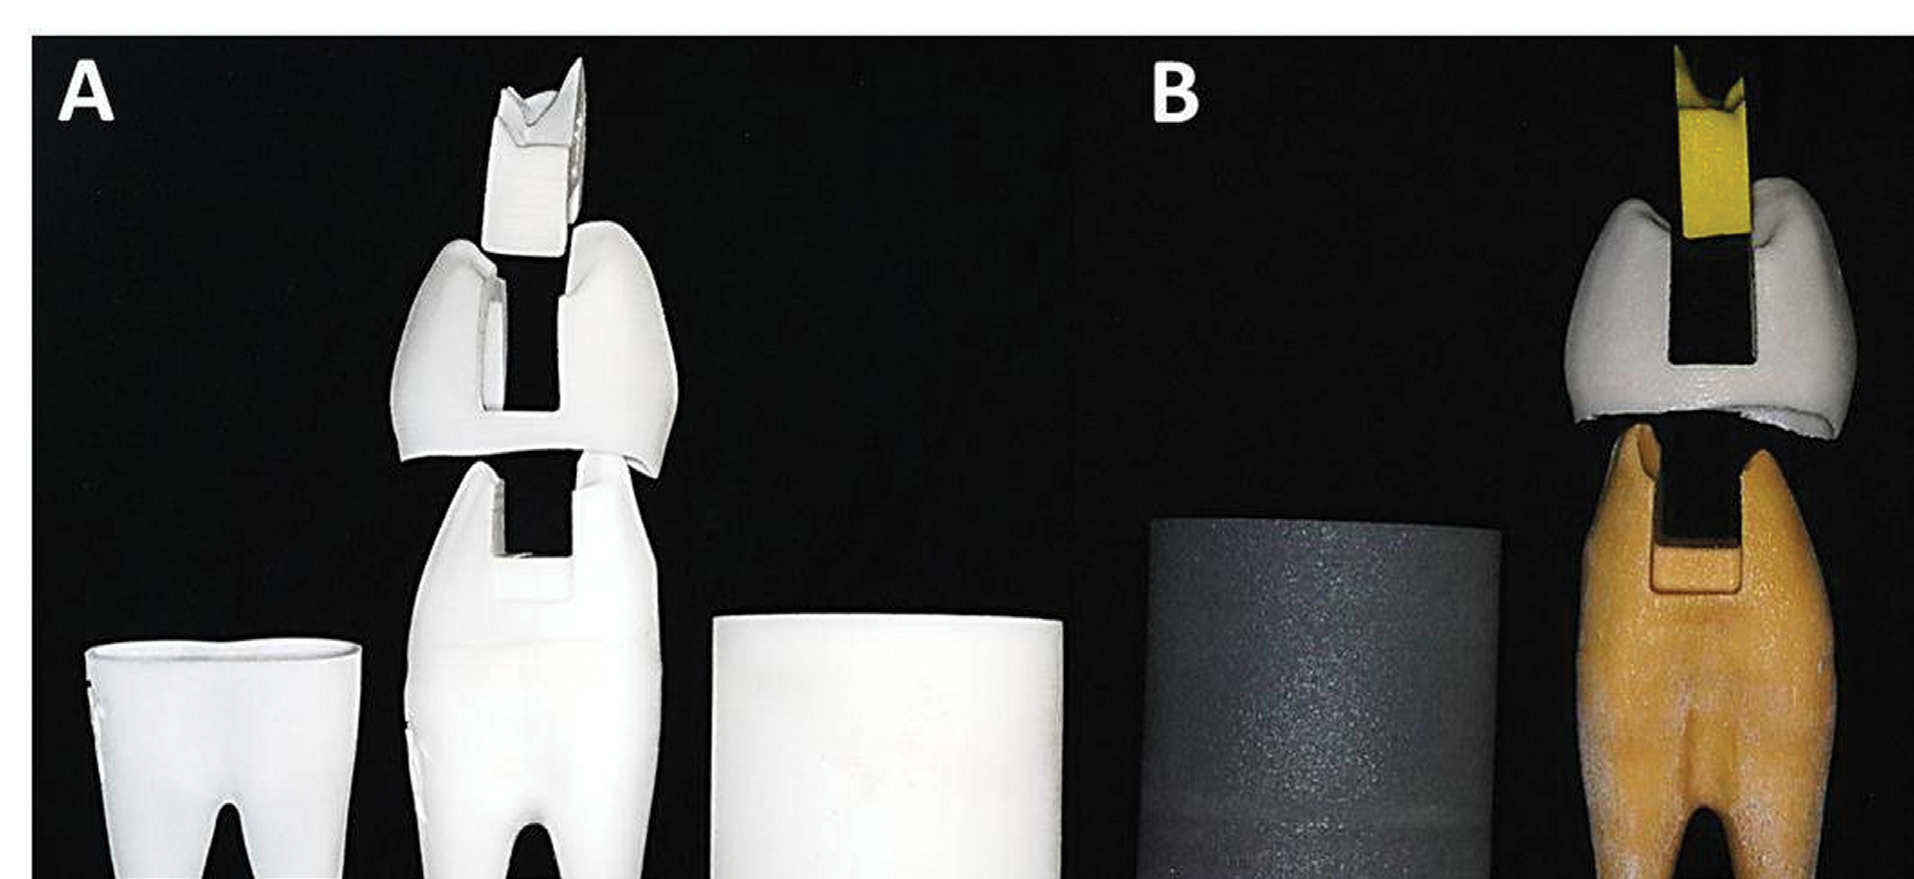
\includegraphics[width=0.8\textwidth, height=\textheight,keepaspectratio]{cavity_prep}
    \caption{Modelli dentali assemblabili rappresentanti delle preparazioni di cavità. Da \emph{Soares et al} \parencite{Reference71}}
    \label{fig:cavity_prep}
    \end{center}
\vspace{-20pt}
\end{figure}
\\ 
Soares et al \parencite{Reference71} ha prodotto modelli di elementi dentari preparati per istruire gli studenti sulle tecniche di preparazione di cavità \ref{fig:cavity_prep}. Altri autori hanno realizzato modelli 3d come supporto pratico ai corsi preclinici, ad esempio Kroger et al \parencite{Reference72} ha realizzato modelli per eseguire rimozioni di carie e realizzazione di provvisori; Reymus et al \parencite{Reference73} ha stampato repliche di elementi dentali con cavità endodontiche per simulare la preparazione endodontica. Il dato comune a questi studi era la valutazione generale positiva dei simulatori stampati in 3D si da parte degli studenti che dei docenti. Le stampanti 3d sono inoltre accolte con piacere dagli studenti e dal personale universitario, come documentato da Walker \parencite{Reference74}.\\
Sono già presenti online diverse librerie in cui è possibile trovare modelli anatomici, come quella fornita dal \emph{NIH} \parencite{Reference75} e quella presente sul sito web \emph{Embodi3d} \parencite{Reference76}. Inoltre le possibilità offerte dal flusso di lavoro qui descritto permettono di creare modelli anatomici originali di casi complessi o procedure particolari a costo ridotto. L'iniziale sforzo nell'uso dei software viene compensato dal ventaglio di possibilità offerte dal workflow in esame come ausilio all'educazione dell'odontoiatra in formazione.

\section{Programmazione dell'intervento chirurgico} 
La programmazione dell'intervento chirurgico è un passo importante per il trattamento del paziente, perché fornisce al team di chirurgia una conoscenza approfondita del caso in esame e permette di valutare l'approccio migliore alla chirurgia. Le tecniche di imaging digitale associate ai modelli 3D sono state sperimentate da diversi autori con l'obbiettivo di fornire al chirurgo un riferimento reale per programmare l'intervento.\\ Modelli che replicano l'anatomia della regione da operare sono stati creati per diverse chirurgie, dalla chirurgia vascolare alla chirurgia ortopedica. Il libro \emph{Medical Modeling} di Bibbs et al \parencite{Reference1} raccoglie una serie di interessanti casi clinici, chirurgici, odontoiatrici e di ricerca che mostrano utilizzo delle tecniche di modellazione medica e prototipazione rapida. Il chirurgo può simulare sui modelli l'esecuzione delle osteotomie, simulare la nuova disposizione dei segmenti ossei e creare guide chirurgiche come ausilio all'intervento \parencite{Reference77}, \parencite{Reference78}.
\begin{figure}[h]
\vspace{-10pt}
	\begin{center}
	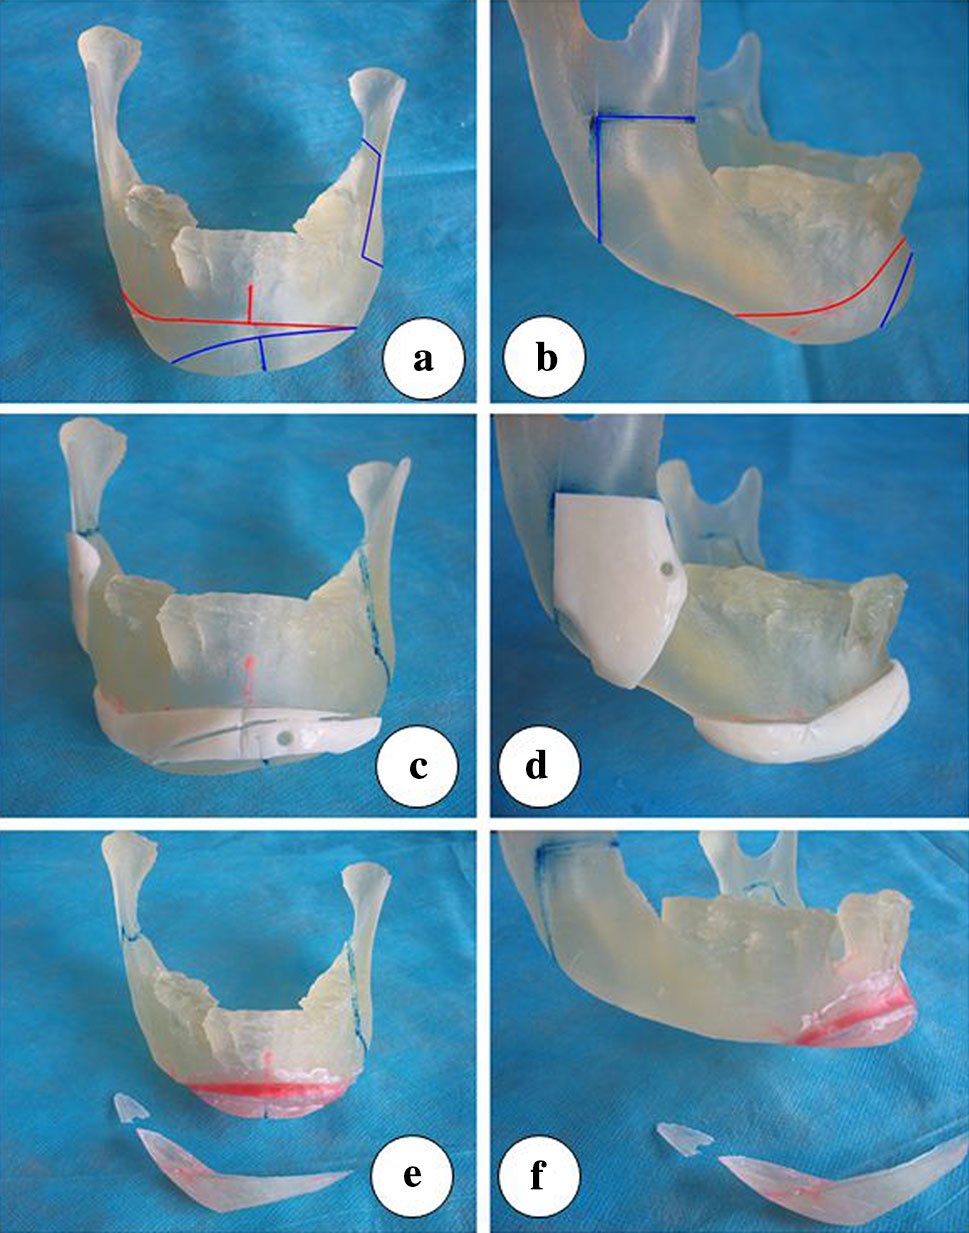
\includegraphics[width=0.5\textwidth,height=\textheight,keepaspectratio]{train_model}
    \caption{Modello per programmazione della chirurgia stampato in 3D.
\textbf{a}: Misure, analisi e linee di osteotomia marcate sul modello (vista frontale).\textbf{b}: Misure, analisi e linee di osteotomia marcate sul modello (vista laterale). \textbf{c}: Realizzazione del template chirurgico (vista frontale). \textbf{d}: Realizzazione del template chirurgico (vista laterale). \textbf{e}: Simulazione chirurgica (vista frontale). \textbf{f}: Simulazione chirurgica (vista laterale). Da \emph{Wang et al} \parencite{Reference20}.}
    \label{fig:train_model}
    \end{center}
\vspace{-20pt}
\end{figure}
\\ 
Ad esempio Wang \parencite{Reference109} ha riportato l'uso di modelli 3d per la programmazione della chirurgia ortognatica mandibolare e per la fabbricazione di guide chirurgiche, notando una maggior velocità e precisione nell'esecuzione dell'osteotomia e nel riposizionamento dei segmenti ossei \ref{fig:train_model}.\\
Il plugin di Blender \emph{OrtogOnBlender} \parencite{Reference64}, \parencite{Reference79} aiuta la programmazione dell'inter\-vento di \emph{chirurgia ortognatica} \ref{fig:ortogon1}, facilitando la simulazione delle osteotomie e permettendo di valutare le conseguenze delle mobilizzazioni ossee sul volto del paziente. Il viso del paziente può essere scannerizzato o rilevato con una serie di fotografie; OrtogOnBlender permette di ricavare modelli 3D attraverso la fotogrammetria, e di utilizzare questi modelli in combinazione con le scansioni TC per avvalersi dei modelli dell'interno e dell'esterno dell'orga\-nismo. In questo modo si possono simulare le conseguenze sul volto del paziente del riposizionamento dei segmenti ossei \parencite{Reference145}.
\begin{figure}[h]
\vspace{-10pt}
	\begin{center}
	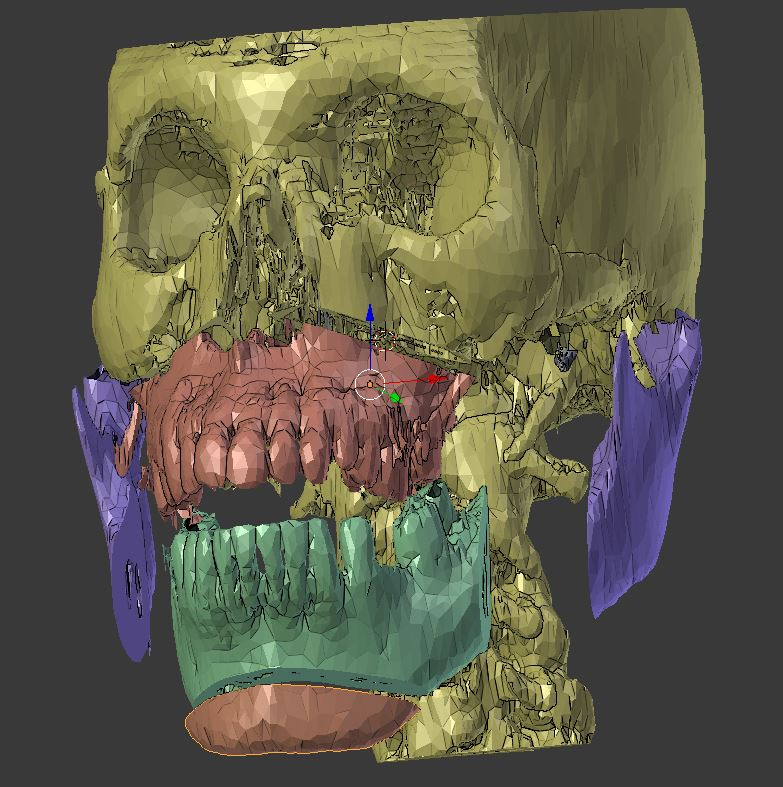
\includegraphics[width=0.6\textwidth,height=\textheight,keepaspectratio]{ortogon1}
    \caption{Osteotomie virtuali eseguite con add-on \emph{OrthogOnBlender}}
    \label{fig:ortogon1}
    \end{center}
\vspace{-20pt}
\end{figure}
\\
La procedura per la preparazione alla simulazione della chirurgia ortognatica con OrtogOnBlender \parencite{Reference80} consiste nel caricamento delle immagini DICOM in Blender, ma può essere utilizzato anche un modello .stl già processato. Il plugin facilità l'effettuazione delle osteotomie digitali mettendo a disposizione dei piani di taglio che vanno posizionati nella posizione desiderata; eseguite le osteotomie digitali possiamo isolare i segmenti e riposizionarli.\\
La gestione delle foto per la ricostruzione in fotogrammetria è molto agevole, basta importare la cartella contenente le foto ed il software automaticamente crea il modello del volto del paziente. Tramite poche operazioni la scansione del viso si allinea con le immagini della TC ed è possibile così la valutazione virtuale della ricollocazione dei mascellari.\\
Le tecnologie di prototipazione rapida sono state usate con successo per la realizzazione di un otturatore chirurgico personalizzato in seguito della rimozione di un carcinoma al mascellare superiore \parencite{Reference81}. \\
Ackland et al \parencite{Reference82} hanno riabilitato di una paziente con artrosi all'\emph{Articolazione Temporo Mandibolare} (ATM) disegnando una protesi personalizzata, sulla quale hanno eseguito simulazioni meccaniche al computer (FEA) per ottimizzarne la posizione ed il fissaggio. Il modello digitale è stato poi stampato in Titanio 6Al4V con una stampante SLS ed impiantato sulla paziente con buoni risultati.\\
L'integrazione delle tecniche digitali e della stampa 3D nel workflow chirurgico possono essere di notevole aiuto al chirurgo per la preparazione all'inter\-vento, soprattutto in casi di chirurgie complesse ed in aree delicate dell'organismo (ad esempio in prossimità di fasci neurovascolari). Queste tecnologie permettono inoltre di personalizzare eventuali dispositivi di riabilitazione, come protesi che si adattano all'anatomia ed alla biomeccanica del paziente. La collaborazione multidisciplinare nella programmazione chirurgica è un tassello portante di questo approccio riabilitativo incentrato sulla personalizzazione.


\section{L'odontoiatria digitale e la stampa 3D}
	
\subsection{Guide chirurgiche implantari}
L'imaging digitale è fondamentale in implantologia per la selezione del sito implantare, mentre le tecniche di modeling e prototipazione rapida permettono di creare velocemente delle guide chirurgiche personalizzate, che possono essere autoclavate ed utilizzate per l'inserimento degli impianti \parencite{Reference83}. Come mostrato da analisi della letteratura, la guida chirurgica permette di operare con maggior precisione rispetto alle procedure d'inserimento manuale dell'impianto. Van Assche \parencite{Reference105} ha effettuato una review della letteratura, dando indicazioni sull'utilizzo delle guide chirurgiche in implantologia (Fig. 34). La posizione dell'impianto inserito con le guide è più predicibile rispetto all'inserimento manuale, e la guida nella fase dell'inserimento dell'impianto ha una precisione maggiore rispetto alla guida delle sole osteotomie, dove solo la preparazione del sito è guidata, mentre il successivo inserimento della fixture è manuale. L'errore medio riscontrato con le guide è di circa 1mm nella posizione d'ingresso, 1,3mm all'apice ed una differenza di angolazione di circa 4 gradi, anche se con una ampia variabilità tra gli studi analizzati.
\begin{figure}[h!]
 
\begin{subfigure}{0.5\textwidth}
\centering
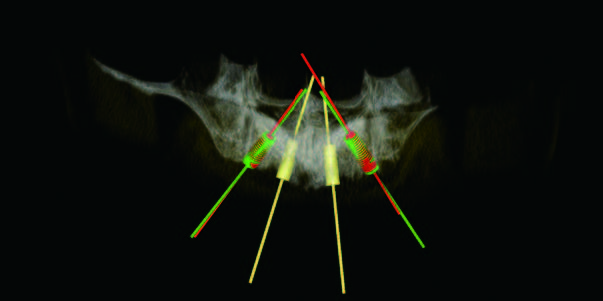
\includegraphics[width=0.9\linewidth, keepaspectratio]{beretta_digital} 
%\caption{Skirt}
\label{fig:beretta_digital}
\end{subfigure}
\begin{subfigure}{0.5\textwidth}
\centering
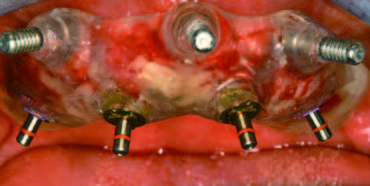
\includegraphics[width=0.9\linewidth, keepaspectratio]{beretta_real}
%\caption{}
\label{fig:beretta_real}
\end{subfigure}

 
\caption{\textbf{A sinistra}: Sovrapposizione tra simulazione degli impianti nella TC preoperatoria (rosso) e scansione postoperatoria con impianti inseriti (verde). \textbf{In basso}: Guida chirurgica per l'arcata madibolare, stabilizzata con miniimpianti. Da \emph{Beretta et al} \parencite{Reference104}.}
\label{fig:Beretta}
\end{figure}
\\
Beretta \parencite{Reference104} ha riscontrato dati simili in letteratura, ma nella sua piccola serie di 14 riabilitazioni implantari eseguite con guide chirurgiche ha trovato errori più bassi. La maggior precisione è da lui imputata ad alcuni accorgimenti, come l'uso di riferimenti extraorali per il corretto posizionamento anatomico, l'uso combinato di scansioni CT e scansioni ottiche nelle procedure di posizionamento, ed il fissaggio intraorale della guida con mini impianti \ref{fig:Beretta}.\\
Secondo i report analizzati l'utilizzo delle guide chirurgiche risulta un valido aiuto alle procedure d'inserimento implantare, tenendo presente un margine di errore adeguato di almeno 2mm da zone sensibili \parencite{Reference104}. L'accuratezza nella produzione delle guide è fondamentale, per cui si deve cercare di ridurre l'errore accumulato tra le operazioni di scansione delle arcate, di design e di manifattura della guida.
 

\subsection{Impianti Anatomici}
In campo implantologico degli autori hanno descritto impianti anatomici da inserire in alveoli postestrattivi (Root Analog Implant). Questi impianti sono realizzati con tecniche CAD/CAM di manifattura additiva o sottrattiva (fresatura), e replicano la morfologia dell'elemento dentario da sostituire. L'anatomia dell'alveolo può essere ottenuta mediante l'uso di una scansione CBCT oppure con la scansione ottica del dente estratto. La scansione ottica richiede di operare in due tempi, essendoci la necessità di estrarre il dente per scansionarlo, creare il modello digitale, stampare l'impianto e riaprire il sito chirurgico per inserirlo. La CBCT preoperatoria permette di pianificare l'intervento, creare l'impianto personalizzato per poi inserirlo subito dopo l'estrazione dell'elemento dentario, in un'unica seduta.
\begin{figure}[h]
\vspace{-10pt}
	\begin{center}
	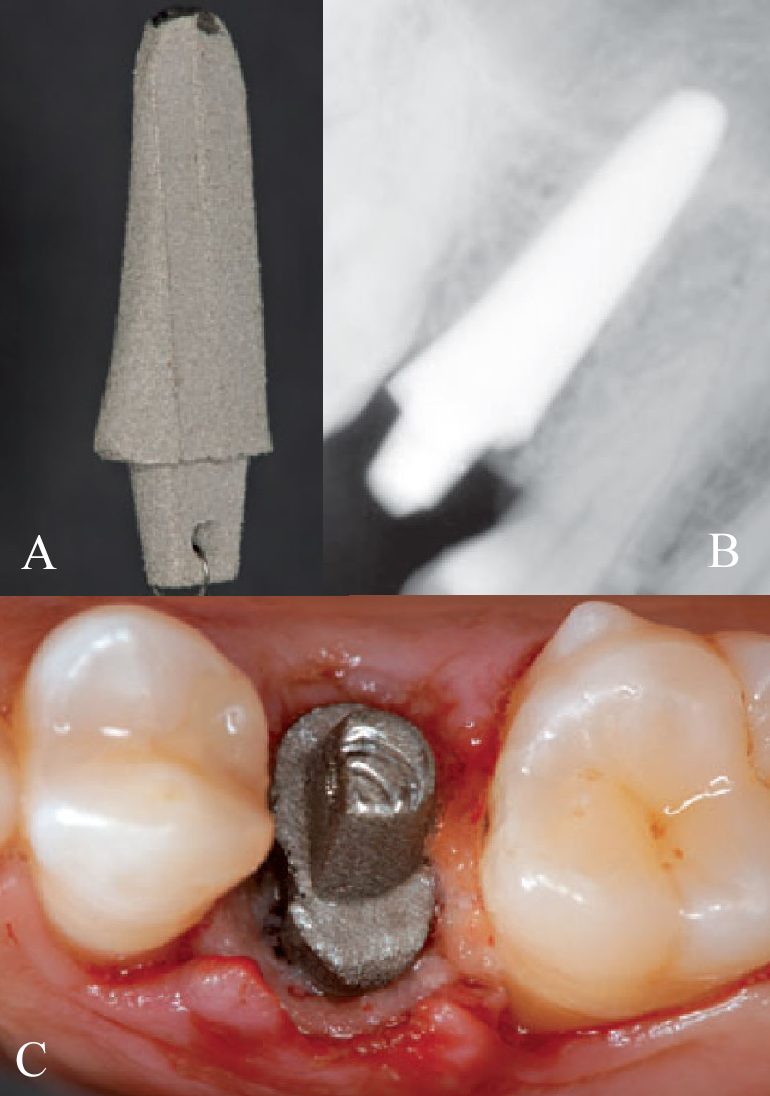
\includegraphics[width=0.5\textwidth,height=\textheight,keepaspectratio]{mangano_implant}
    \caption{Impianti anatomici realizzati con tecnologia DLMF. \textbf{A}: impianto anatomico in titanio. \textbf{B}: radiografia dell'impianto inserito in alveolo. \textbf{C}: aspetto clinico dell'impianto in cavo orale. Da \emph{Mangano et al} \parencite{Reference84}}
    \label{fig:mangano_implant}
    \end{center}
\vspace{-20pt}
\end{figure}
\\
Mangano \parencite{Reference84} ha utilizzato ricostruzioni CBCT per realizzare l'impianto personalizzato per mezzo della tecnologia di stampa DLMF (\emph{Direct Laser Metal Forming}), che usa un laser per sinterizzare layer di particelle di titanio dell'altezza di 0.2mm \ref{fig:mangano_implant}. L'impianto è stato protesizzato in maniera definitiva ed al controllo annuale si notava il mantenimento dei tessuti perimplantari.\\
Mangano \parencite{Reference85} ha poi eseguito uno studio su 15 pazienti, utilizzando impianti anatomici in titanio. Nonostante siano necessari ulteriori studi, il lavoro ha mostrato come gli impianti anatomici in titanio realizzati con tecnica DLMS (\emph{Direct Laser Metal Sintering}) possano essere una opzione di trattamento per casi di riabilitazione postestrattiva di elementi dentari in cui sia possibile una avulsione atraumatica, dove le corticali vengono mantenute intatte. \\
Pirker \parencite{Reference86} ha modificato la radice del dente estratto con l'aggiunta di macroritenzioni in composito sulla porzione distale e prossimale, lasciando inalterate la superficie vestibolare e la superficie linguale della radice. La radice così modificata è stata scansionata con uno scanner ottico, ed il modello digitale ottenuto è stato lievemente ridotto nel diametro della regione vestibolare e della regione linguale (tra 0.1 e 0.3 mm) per limitare il rischio di frattura delle corticali alveolari. L'impianto è stato poi prodotto in zirconia mediante un fresatore CAD-CAM ed impiantato nell'alveolo \ref{fig:bioimplant}. La stabilità primaria era ottimale, grazie all'uso delle macroritenzioni interdentali.  Al follow up a 2 anni non c'erano segni di riassorbimento osseo e retrazione gengivale, segno anche di una corretta distribuzione degli stress sulla parete dell'alveolo.
\begin{figure}[h]
\vspace{-10pt}
	\begin{center}
	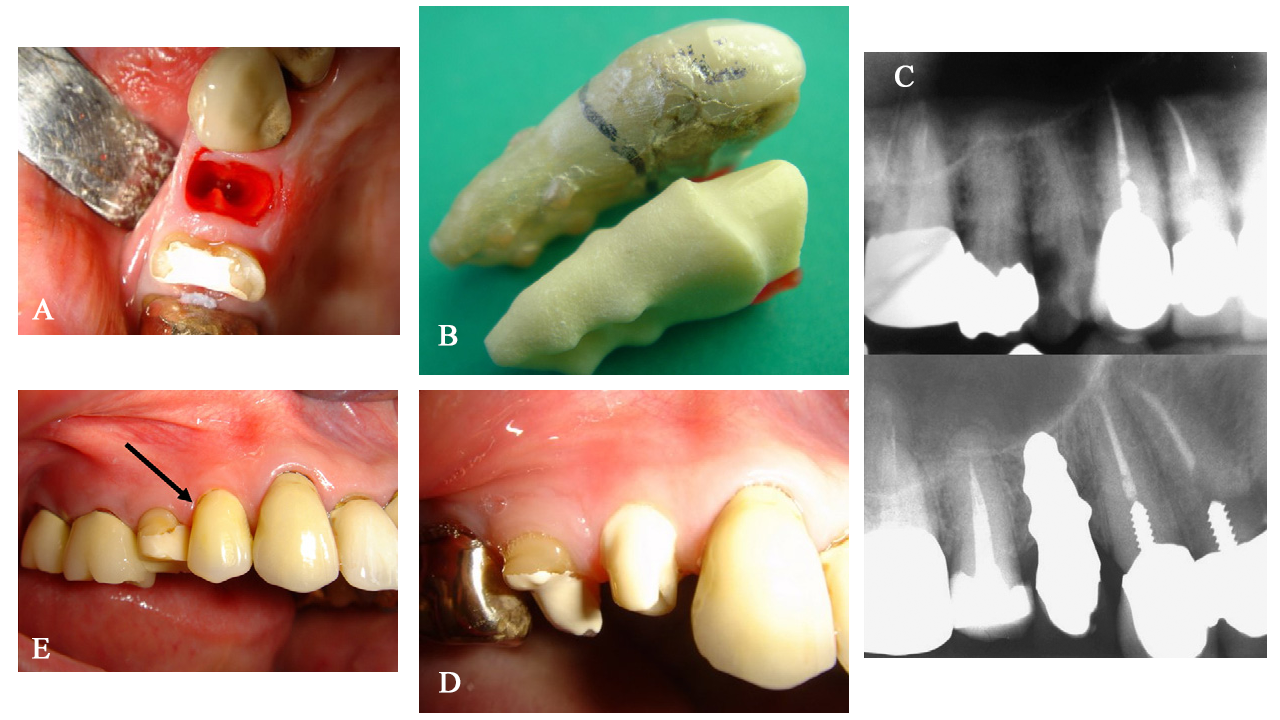
\includegraphics[width=0.9\textwidth,height=\textheight,keepaspectratio]{bioimplant}
    \caption{Inserimento e controllo impianto anatomico in zirconia. A: alveolo intatto di premolare estratto atraumaticamente. B: Elemento dentario estratto con ritenzioni simulate con composito, e impianto anatomico in zirconia con macroritenzioni. C: Radiografia pretrattamento (in alto) e post trattamento, con impianto anatomico inserito (in basso). D: impianto anatomico inserito. E: controllo clinico dopo 2 anni dall'inserimento dell'impianto; si nota il mantenimento dei tessuti parodontali. Da \emph{Pirker et al} \parencite{Reference86}}
    \label{fig:bioimplant}
    \end{center}
\vspace{-30pt}
\end{figure}
\\

Lo stesso autore ha poi effettuato una comparazione tra diverse topografie di impianti anatomici in zirconia realizzati con tecnologia CAD-CAM in un due gruppi di pazienti \parencite{Reference87}. Un gruppo di pazienti veniva riabilitato con impianti anatomici con una superficie rugosa realizzata mediante sabbiatura, mentre il secondo gruppo era trattato con impianti sabbiati su cui erano presenti macroritenzioni sulle superfici interdentali. Il gruppo di impianti sabbiati ha mostrato un tasso di successo dello 0\%, con tutti i 6 impianti inseriti che sono falliti prima di essere protesizzati. Il gruppo trattato con impianti con macroritenzioni ha mostrato un tasso di successo del 92\% a due anni, con solo un impianto perso su 12 inseriti. Il fallimento degli impianti con microritenzioni è stato imputato alla pressione uniforme esercitata dall'impianto sulle pareti dell'alveolo, mente ne caso con macroritenzioni la distribuzione del carico in aree definite ha permesso di ridurre lo stress sull'osso, favorendo l'osteointegrazione dell'impianto. \\
Patankar \parencite{Reference88} ha replicato la struttura anatomica in zirconia di Pirker con macroritenzioni interdentali, per la riabilitazione di un premolare inferiore, con un risultato positivo.\\

\begin{wrapfigure} {R} {0.4\textwidth}
\vspace{-20pt}
	\begin{center}
	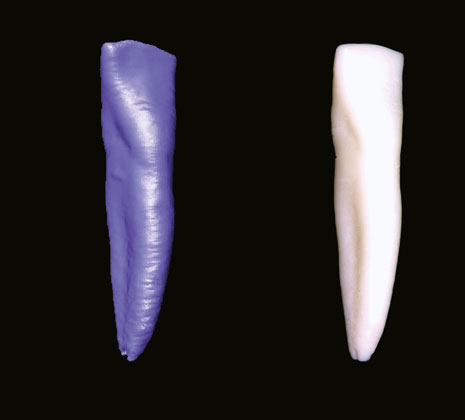
\includegraphics[width=0.4\textwidth, height=\textheight,keepaspectratio]{moin_dlp_zirconia}
    \caption{a sinistra modello CAD dell'elemento dentario. A destra modello dentario  in zirconia stampato stampato con tecnica DLP. Da \emph{Moin et al} \parencite{Reference89}}
    \label{fig:moin_dlp_zirconia}
    \end{center}
\vspace{-20pt}
\end{wrapfigure}

Moin \parencite{Reference89} ha utilizzato la tecnica di produzione additiva Digital Light Processing (DLP) per realizzare una replica in zirconia di un elemento dentale \ref{fig:moin_dlp_zirconia}. L'autore ha poi comparato digitalmente il modello CAD della replica, la scansione della replica stampata in zirconia e la scansione dell'elemento dentario originale, constatando l'adeguata precisione della tecnologia DLP per la fabbricazione additiva di manufatti in zirconia. \\
La produzione di manufatti in ceramica è attualmente possibile anche tramite la tecnica di stampa per estrusione, come documentato da Nötzel \parencite{Reference97}. Il processo usato consiste nella produzione di un filamento composto da paraffina, LDPE e particelle di Al2O3; il filamento viene stampato per estrusione a formare l'oggetto, che viene poi sottoposto a trattamento chimico e termico per la rimozione del medium in cui sono disperse le particelle di Al2O3 ed infine sinterizzato in forno a dare il manufatto finale. La stampa per estrusione di manufatti ceramici resta ancora da valutare nell'ambito della produzione di manufatti odontoiatrici. \\

Questi report ci dimostrano che, avvalendosi di tecniche digitali, la produzione di impianti anatomici è ormai possibile in maniera precisa e con l'utilizzo di biomateriali che favoriscono l'osteointegrazione ed una riabilitazione estetica e funzionale.\\
Importante risulta in quest'ottica la corretta determinazione della morfologia dell'alveolo e dell'impianto sostitutivo, e della distribuzione delle forze masticatorie sull'osso alveolare. Una avulsione atraumatica sta alla base della riabilitazione con impianti anatomici, perché eventuali traumi all'alveolo risultano in riassorbimenti ossei e retrazioni gengivali, con conseguente degradazione delle caratteristiche estetiche della riabilitazione. La distribuzione delle forze sull'alveolo è anch'essa da attenzionare.\\ Con gli impianti anatomici cerchiamo la stabilità primaria per mezzo della congruità dimensionale tra l'alveolo e l'impianto anatomico; è stato dimostrato che un eccessivo stress sulle pareti dell'alveolo causa il fallimento implantare, probabilmente per riduzione dell'apporto ematico al sito implantare ed all'osso circostante, che va incontro a riassorbimento. Ulteriori studi sono necessari per verificare la sicurezza e la standardizzazione delle procedure attualmente presenti, ma gli impianti anatomici potrebbero permettere, in casi selezionati, una soluzione funzionale ed estetica al problema del paziente, ed agevolare la risoluzione di casi di impianti postestrattivi mantenendo alti standard estetici.

\subsection{Protesi}
La prototipazione rapida è stata utilizzata sia in protesi fissa che in protesi rimovibile, per la realizzazione di restauri provvisori stampati, guide estetiche, mockup e per la realizzazione di scheletrati. Sono state usate varie tecnologie di manifattura additiva e vari materiali.\\
Tahayeri \parencite{Reference98} ha testato varie caratteristiche della stampa SLA con resine specifiche per l'uso dentale (NextDent), valutando l'influenza di alcuni parametri sulla precisione di stampa, sulle proprietà meccaniche e sul grado di conversione della resina. I provini stampati si sono dimostrati nel range di precisione richiesto per l'uso clinico, così come lo erano le proprietà meccaniche degli stessi campioni. L'autore ha notato differenze tra le caratteristiche nella stampa di varie resine dentali realizzate dallo stesso produttore, nonché differenti intensità del laser durante la polimerizzazione delle varie resine, in base al colore più o meno scuro della resina e del relativo tasso di assorbimento della luce. Una selezione di resine e stampanti ottimizzate per l'uso congiunto potrebbe migliorare ulteriormente la precisione di stampa; migliori risultati potrebbero derivare dalla fine regolazione delle caratteristiche della stampante in fase di stampa.
Da considerare che, secondo le indicazioni del produttore, la resina avrebbe dovuto subire un secondo passaggio di polimerizzazione dopo la stampa, cosa che gli autori non hanno eseguito per accelerare l'eventuale processo di produzione del provvisorio. Nonostante ciò le proprietà meccaniche della resina non post-polimerizzata si sono mostrate adeguate a resistere ai carichi intraorali. \\
Katreva \parencite{Reference99} ha realizzato un flusso di lavoro che ha integrato l'uso di modelli di lavoro stampati in 3D, la stampa 3D dei provvisori e la stampa della protesi definitiva per la conversione in ceramica pressata.\\
Revilla-León \parencite{Reference100} ha utilizzato un workflow digitale per la scansione delle impronte, la realizzazione della ceratura diagnostica, la stampa di una guida per la realizzazione dei provvisori ed infine per la produzione delle veneer, utili alla riabilitazione estetica e funzionale del settore anteriore dell'arcata mascellare. La guida per la realizzazione dei provvisori è stata realizzata mediante tecnica di stampa 3D DLP, mentre le veneer in disilicato di litio definitive sono state fresate al CAD-CAM.\\
Alharbi \parencite{Reference101} ha valutato la possibilità di realizzare corone protesiche con tecnica di stampa SLA. L'autore ha misurato l'accuratezza della corona stampata a varie angolazioni rispetto al piano e con l'uso di supporti di diverse dimensioni. Lo stesso gruppo di ricerca ha poi valutato l'accuratezza nella stampa di corone per mezzo della tecnica di stampa DLP \parencite{Reference102}. Entrambe le tecnologie si sono rivelate precise, con la stampa SLA che ha mostrato un maggior accuratezza nella replica della morfologia del modello digitale. Entrambe le tecnologie sono interessanti per l'impiego in odontoiatria, ma è necessario compiere ulteriori studi sull'influenza dei parametri di stampa sul modello finale ed approfondire le proprietà delle resine dentali.\\
\begin{wrapfigure} {R} {0.4\textwidth}
\vspace{-20pt}
	\begin{center}
	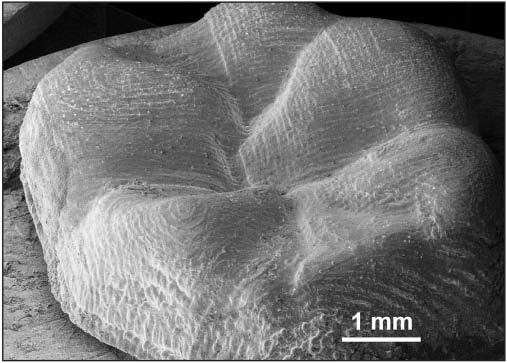
\includegraphics[width=0.4\textwidth, height=\textheight,keepaspectratio]{zircon_crown}
    \caption{Corona in zirconia realizzata con stampa ink-jet. Da \emph{Ebert et al} \parencite{Reference106}}
    \label{fig:zircon_crown}
    \end{center}
\vspace{-20pt}
\end{wrapfigure}

Ebert ha stampato corone in zirconia per mezzo di una stampante personalizzata, usando la tecnica ink-jet. Per realizzare la corona, una soluzione contenente zirconia veniva depositata strato dopo strato a formare il manufatto, che veniva poi sinterizzato in forno \ref{fig:zircon_crown}. Questo studio ha dimostrato che corone in zirconia con capacità meccaniche e precisione utili all'utilizzo clinico possono essere realizzate mediante tecnica di manifattura additiva ink-jet \parencite{Reference106}.\\
Alharbi \parencite{Reference107} ha valutato l'utilizzo della manifattura additiva in protesi, analizzando vari report e studi incentrati sulla protesi fissa e la protesi mobile parziale e totale. L'autore ha riportato che le sottostrutture metalliche realizzate con la metodica SLS (\emph{Selective Laser Sintering}) sono equivalenti o più precise rispetto alle procedure classiche di fusione per quanto riguarda il gap tra sottostruttura metallica e moncone dentale; allo stesso modo le proprietà meccaniche dei manufatti SLS erano equivalenti o migliori rispetto a quelli realizzati con le procedure classiche. Strutture metalliche per la realizzazione di protesi parziali rimovibili sono state prodotte per mezzo della manifattura additiva per via diretta o indiretta. La manifattura diretta consiste nella stampa del design per mezzo di processi SLS; la manifattura indiretta consiste nella realizzazione del manufatto in resina calcinabile per mezzo della stampa SLA oppure DLP, l'integrazione del modello calcinabile in materiale refrattario e la successiva colatura del metallo o della lega per la realizzazione del framework metallico. Entrambe le tecniche per la realizzazione dei framework per protesi removibile hanno mostrato una accuratezza accettabile, anche se i risultati derivano principalmente da studi in vitro e case report.\\
Lin \parencite{Reference108} ha dimostrato una tecnica per la realizzazione di protesi mobili totali provvisorie attraverso un protocollo digitale che prevede la scansione ottica, la ceratura diagnostica digitale della protesi, la stampa della base protesica e rispettiva arcata dentaria in fasi separate e con resine di colore e caratteristiche adatte, ed infine l'unione di arcata e base protesica \ref{fig:separ_full_prot}. Lo studio non ne ha testato l'uso sul paziente e non sono presenti ulteriori report della performance clinica di protesi mobili totali provvisorie realizzate con questa procedura e questi materiali. Questo concept potrebbe essere approfondito, valutando l'accuratezza rispetto agli altri metodi di fabbricazione disponibili e la durata della protesi nel tempo, sia dal punto di vista del colore che dell'usura della resina.\\
I dati disponibili sulle tecniche di programmazione digitale del trattamento e l'utilizzo delle tecnologie di manifattura additiva mostrano prospettive promettenti in odontoiatria, sia per la produzione di provvisori \parencite{Reference125} che di protesi removibili \parencite{Reference107}. Ulteriori studi e valutazioni con follow-up più lunghi sono comunque necessari prima di un'ampia applicazione clinica della tecnologia.  Resta inoltre poco esplorata la possibilità di produrre manufatti definitivi in ceramica o zirconia, possibilmente realizzabili con tecnologie come la SLS  o la stampa inkjet.
\begin{figure}[h]
\vspace{-10pt}
	\begin{center}
	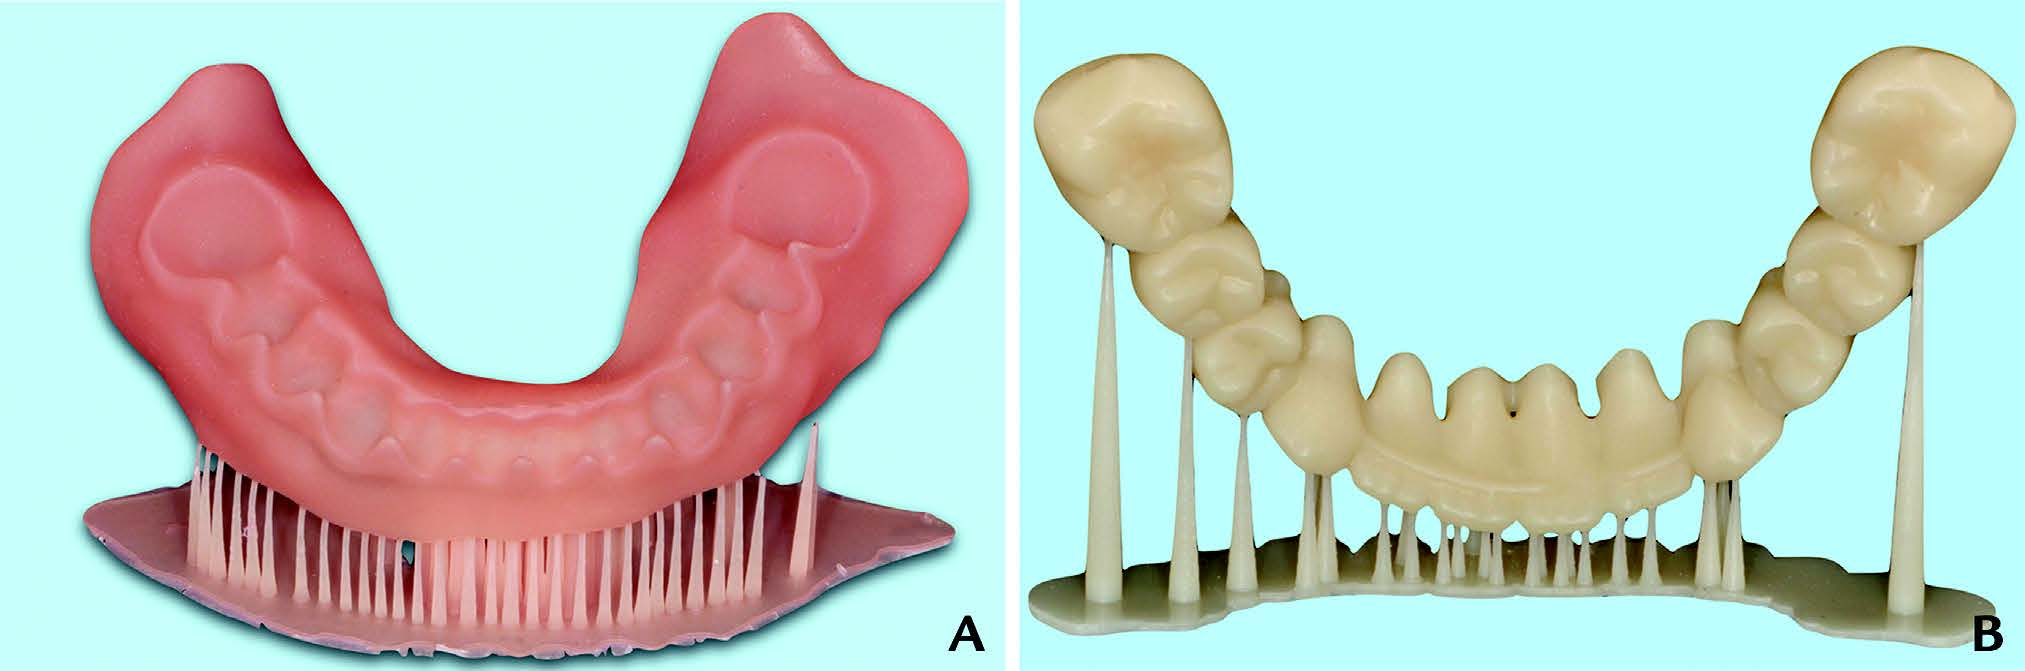
\includegraphics[width=0.9\textwidth,height=\textheight,keepaspectratio]{separ_full_prot}
    \caption{Componenti di Protesi mobile totale provvisoria realizzati con design digitale e stampante 3D DLP. Da \emph{Lin et al} \parencite{Reference108}}
    \label{fig:separ_full_prot}
    \end{center}
\vspace{-30pt}
\end{figure}

\subsection{Ortodonzia} 
L'ortodonzia è una delle branche dell'odontoiatria che più può avvalersi delle nuove possibilità di programmazione digitale del trattamento e dell'uso di tecnologie di manifattura additiva. La terapia ortodontica è classicamente programmata per mezzo di teleradiografie, modelli in gesso in articolatore e set di foto del paziente, oltre alla fondamentale valutazione clinica e funzionale. Le complesse relazioni tra le ossa del cranio coinvolte nella funzione orale sono difficilmente analizzabili in maniera adeguata su delle radiografie bidimensionali e con dei modelli in gesso, soprattutto se il trattamento prevede una fase chirurgica.\\
La terapia ortodontica digitale può avvalersi della possibilità di stampare brackets personalizzati \parencite{Reference115} e guide chirurgiche per l'inserimento di impianti ortodontici \parencite{Reference116} \ref{fig:stent_miniscrew}. La stampa 3d facilita anche la produzione di guide per il posizionamento dei brackets nel paziente \parencite{Reference127}, che favoriscono un posizionamento veloce e preciso degli stessi, e di strumenti ausiliari personalizzati \parencite{Reference126}. I brackets personalizzati sono stati realizzati da Krey attraverso il software FreeCAD ed un processo di stampa DLP \ref{fig:design_brackt}. Con la stessa tecnica è stato stampato uno splint di posizionamento, precedentemente progettato virtualmente, che ha permesso di posizionare i brackets in maniera rapida e precisa. Scansioni intraorali ad intervalli di tempo sono state effettuate e comparate in MeshLab per verificare lo spostamento ortodontico degli elementi dentali; anche lo splint di ritenzione post trattamento è stato progettato virtualmente e stampato in 3D.\\
\begin{figure}[h!]
 
\begin{subfigure}{0.5\textwidth}
\centering
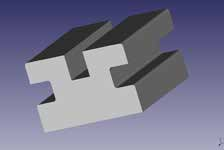
\includegraphics[width=0.9\linewidth, keepaspectratio]{design_brackt} 
\caption{Design CAD del bracket.}
\label{fig:design_brackt}
\end{subfigure}
\begin{subfigure}{0.5\textwidth}
\centering
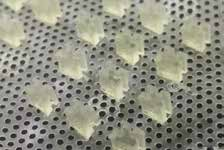
\includegraphics[width=0.9\linewidth, keepaspectratio]{printd_brackt}
\caption{Brackets stampati.}
\label{fig:printd_brackt}
\end{subfigure}
\begin{subfigure}{0.5\textwidth}
\centering
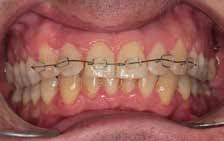
\includegraphics[width=0.9\linewidth, keepaspectratio]{working_brackt}
\caption{Brackets stampati in funzione all'interno del cavo orale.}
\label{fig:working_brackt}
\end{subfigure}
\begin{subfigure}{0.5\textwidth}
\centering
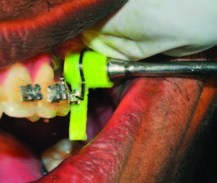
\includegraphics[width=0.7\linewidth, keepaspectratio]{stent_miniscrew}
\caption{Guida per l'inserimento di impianti ortodontici stampata in 3D}
\label{fig:stent_miniscrew}
\end{subfigure}
\caption{A, B e C da \emph{Krey et al} \parencite{Reference115}, D da \emph{Ahamed et al} \parencite{Reference116}}
\label{fig:3d_ortho}
\end{figure}


Questo è stato uno studio di prova con brackets \emph{edgewise} stampati in resina fotopolimerizzabile; gli autori hanno suggerito la possibiltà di rivedere parte del design per ottimizzare la resistenza dei brackets. Il report è in generale positivo e apre alla possibilità di un cambio radicale nel modo in cui l'ortodonzia con apparecchi fissi possa essere eseguita nello studio odontoiatrico, con il passaggio dall'uso di brackets generici a brackets personalizzati realizzabili in ambulatorio.\\
Nella moderna pratica odontoiatrica l'uso di modelli in gesso è spesso affiancato da scansioni digitali e dalla stampa 3d del modello. Diversi autori hanno valutato la precisione dei modelli realizzati con tecniche di manifattura additiva, con risultati diversi. Dietrich \parencite{Reference112} ha valutato la precisione e l'accuratezza di modelli dentali realizzati con stampa polyjet e con tecnica SLA. I modelli stampati sono stati scannerizzati e valutati via software per valutarne la discrepanza con l'originale. Entrambi i metodi di stampa si sono rivelati capaci di una accuratezza di stampa adeguata all'utilizzo ortodontico, con un errore massimo rilevato di circa \SI{100}{\micro\metre}.\\
Wan Hassan \parencite{Reference113} ha comparato manualmente, per mezzo di un calibro, modelli di arcate di pazienti con affollamento dentale, realizzati in gesso e stampati con tecnologia SLA. L'autore ha decretato i modelli non adatti all'uso ortodontico per via di una discrepanza di circa 1mm rispetto all'originale. L'autore riferisce che la scansione digitale dei modelli in gesso risultava in una perdita di dettaglio, inoltre le misurazioni con calibro risultavano a volte non semplici da effettuare per via dell'affollamento. Entrambe queste condizioni potrebbero aver contribuito all'errore riportato. Anche apparecchiature rimovibili possono essere fabbricate con la stampa 3d \parencite{Reference111}. Sono inoltre state usate guide chirurgiche stampate in 3d per effettuare osteotomie corticali allo scopo di accelerare i movimenti ortodontici \parencite{Reference114}.\\
Di rilievo è la possibilità di integrazione che l'ortodonzia digitale ci permette anche dal punto di vista biomeccanico. L'uso di scansioni ottiche e CBCT permette di avere dettagliate informazioni sulla struttura del paziente. I movimenti ortodontici si basano su principi biologici e fisici, dove vengono utilizzate forze controllate per attivare il processo di rimodellamento osseo, il quale permette il movimento dell'elemento dentario. Questi fattori potrebbero essere indagati integrando i dati anatomici (ossa, muscoli, legamenti, organi) ed i dati funzionali (forza masticatoria, caratteristiche meccaniche dei tessuti e materiali coinvolti, range di movimento mandibolare...) per simulare in silico il trattamento, fornendo al paziente un trattamento personalizzato secondo le sue caratteristiche biologiche e di risposta \parencite{Reference110}, \parencite{Reference140}.
\begin{figure}[h]
\vspace{-10pt}
	\begin{center}
	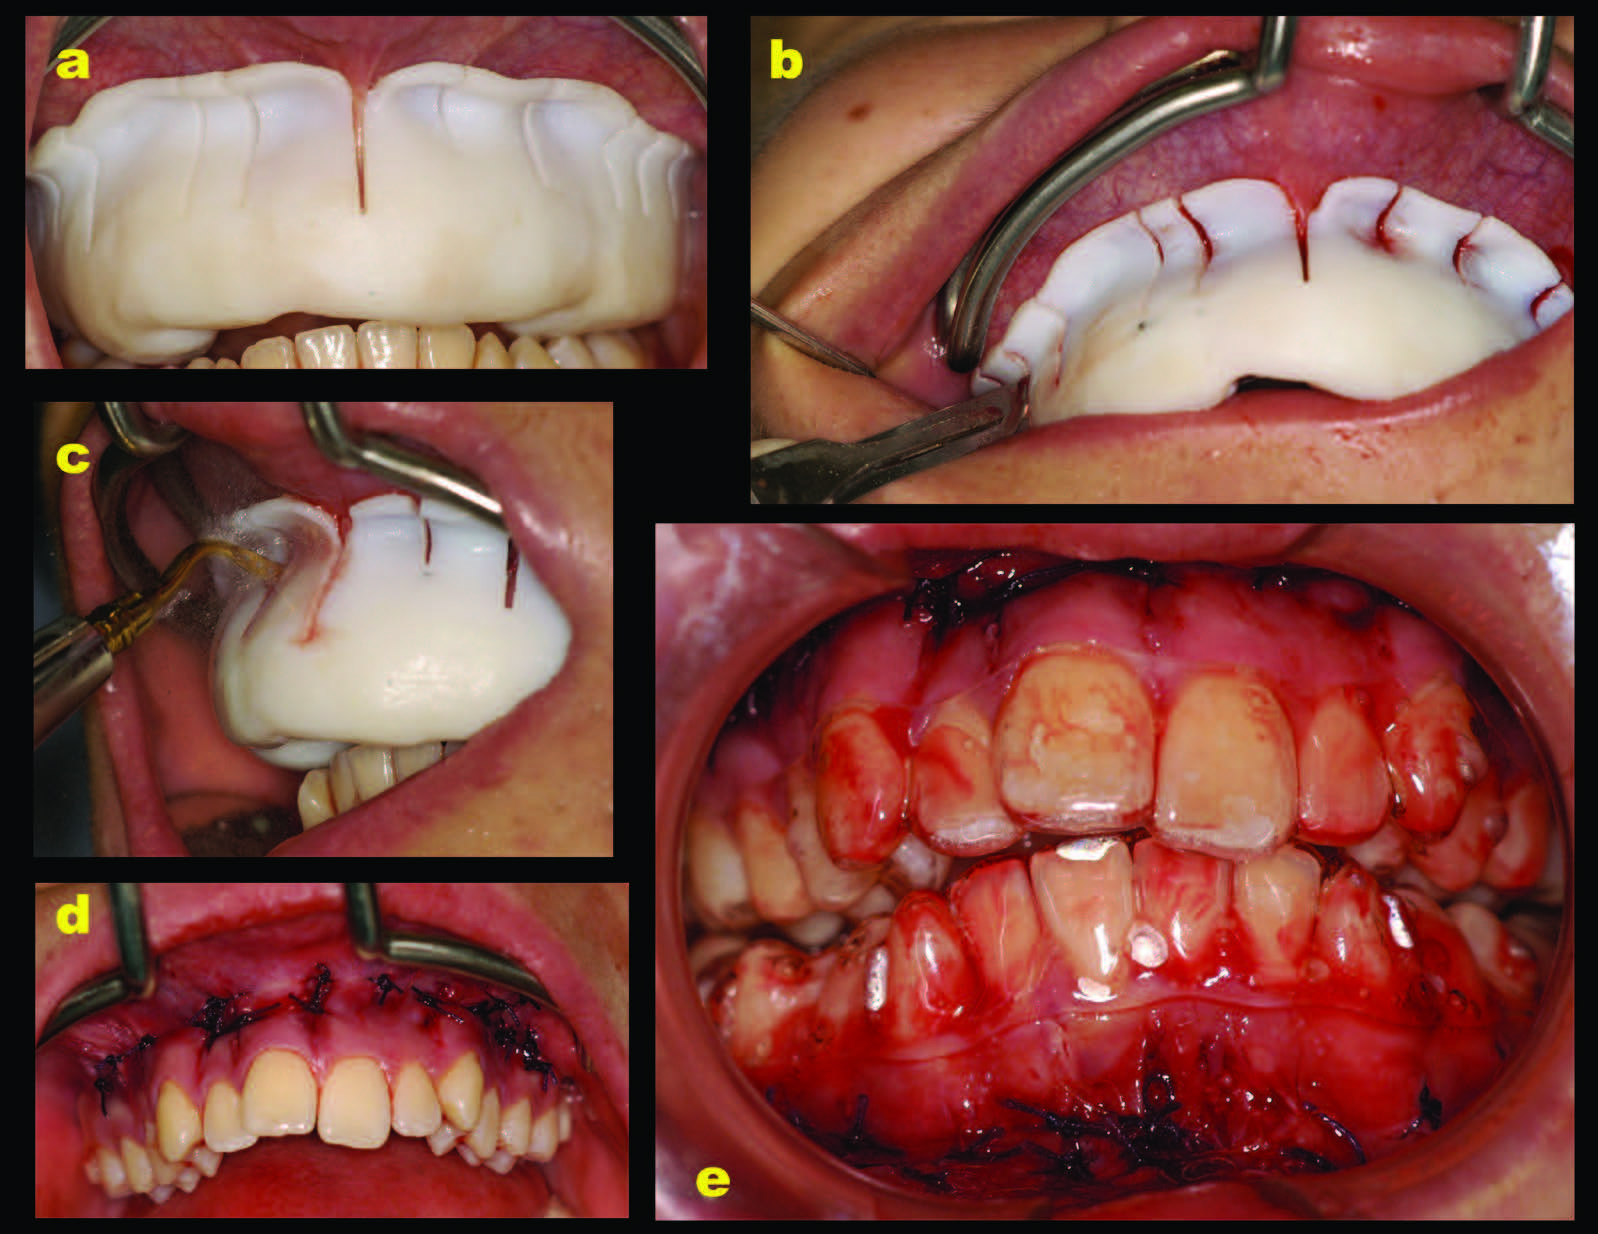
\includegraphics[width=0.9\textwidth, keepaspectratio]{guide}
    \caption{Posizionamento della guida chirurgica stampata in 3D per l'esecuzione di osteotomie flapless. \textbf{a}: Valutazione della stabilità intraorale. \textbf{b}: incisioni verticali della gengiva con bisturi n15. \textbf{c}: corticotomie verticali eseguite usando uno strumento piezoelettrico. \textbf{d}: sutura delle incisioni. \textbf{e}: posizionamento degli allineatori trasparenti dopo la chirurgia. Da \emph{Cassetta et al} \parencite{Reference114}.}
    \label{fig:guide}
	\end{center}
\vspace{-20pt}
\end{figure}

 
  
% Chapter Template

\chapter{Scaffold} % Main chapter title

\label{Chapter7} % Change X to a consecutive number; for referencing this chapter elsewhere, use \ref{ChapterX}

 %----------------------------------------------------
 
The scaffolds are three-dimensional supports that provide cells with an environment in which adhere, differentiate and multiply. Tissue engineering and scaffolds have been developed with the aim of promoting the regeneration of damaged tissues of the body, to solve the problems related to \emph{autologous grafts} and \emph{donor transplants}. \\ Autologous grafts ( i.e. of skin or bone) require longer surgical time and are more invasive (due to the tissue harvesting from a donor site and the implantation in the damaged site). Furthermore, the tissue in the donor site is not always sufficient to regenerate the damaged tissue. Regards to the homologous grafts (from donor of the same species) the concern is in the scarcity of donors and the biological risk of infection and rejection. \\
To provide the best environment for each group of cells to grown, scaffolds made from a wide variety of materials have been described. Each tissue is in fact unique for mechanical and functional properties, as well as for its micro and macrostructure. \\ The introduction of additive manufacturing techniques in the production of scaffolds has brought novelty in the materials used and combinations of these, and has made possible the exploration of complex designs. The scaffolds can be made of biological polymers, synthetic polymers, ceramic materials and combinations of these \parencites{Reference128}. \\
To promote cell survival, the spread of cells and nutrients and the removal of metabolites and waste products must be facilitated by the scaffold structure. The \emph{porosity} of the scaffold is therefore a fundamental parameter, along with the \emph{porosity interconnection} (that describes how the porosities are connected each other inside the volume's boundary). Growth factors and regulatory proteins of cell adhesion can be integrated into scaffolds, to facilitate cell distribution and regulate it in the case of \emph{multiphase scaffolds} \parencite{Reference129}. The scaffold must also be resorbable, and the rate of resorption must be in accordance with the regeneration rate of the tissue to be repaired; the goal of the scaffolds is indeed to stimulate the complete regeneration of the tissue, with the total resorption of the scaffold in the implant site. \\
Among the most recently used dental scaffolds we find ceramic particles such as \emph{tricalcium phosphate} (TCP, TriCalcium Phosphate), \emph{Hydroxyapatite} (HA) and MTA. These materials are used for bone regeneration, along with the collagen or PTFE membranes used to compartmentalize the regeneration site. The ceramic particles form a porous structure that is held together by the blood clot, promoting the spread of cells and nutrients and stimulating bone production. \\ The chemical composition of these granular materials is similar to that of bone, the high roughness of the surface allows the stabilization of the clot, the adsorption of growth factors and increase cell adhesion. However, the porosity of these materials is not tunable, because it depends on the aggregation that is randomly created during the formation of the blood clot. The resulting clot is also unstable and unsuitable to support mechanical loads during the early consolidation steps \parencite{Reference131}. The rate of resorption of some of these materials is slow and they often stay in the site for a long time. \\
The use of three-dimensional scaffolds has therefore tried to overcome these limitations, trying to provide an optimal solution to these problems and to increase the predictability of the regenerative treatment. The introduction of additive manufacturing has made it possible to have greater control over the scaffold architecture, leading to encouraging results \parencite{Reference136}, \parencite{Reference137}.\\

\begin{figure}[h]
\vspace{-10pt}
	\begin{center}
	\includegraphics[width=0.6\textwidth, keepaspectratio]{scaf_paro}
    \caption{Scaffold for periodontal regeneration developed by \emph{Rasperini et al} \parencite{Reference134}.}
    \label{fig:scaf_paro}
	\end{center}
\vspace{-20pt}
\end{figure}

Structures in OCT (\emph{octacalcium phosphate}) are \emph{\ textbf {ostoinductive}}, that is, they stimulate the cells already in the damaged site to osteoblastic differentiation \parencite{Reference130}. Osteoinduction is also a property of a composite scaffold made of polycaprolactone and decellularized bone \parencite{Reference132}. A bioactive hydrogel composed of alginate, gelatin and OCT (56, 14, 30 wt\%, respectively) containing Vancomycin or Doxorubicin was tested in order to realize scaffolds with \emph{antibacterial} and \emph{antitumorals} properties, with interesting results \parencite{Reference133}. \\
Lastly, there are promising recent attempts to realize three-dimensional scaffolds for the periodontal ligament regeneration. The periodontal regeneration requires reconstitution of alveolar bone, periodontal ligament and dental cement, so the classic concept of compartmentalization of the periodontal defect has been extended with the use of three-dimensional anisotropic scaffolds, with different compartments and geometric and structural characteristics specific to the tissue to regenerate, such as the guides to direct the regeneration of spatially oriented periodontal fibers. \\
Several authors have made this type of scaffold, and in one case this was tested clinically on the patient; the scaffold was removed after 13 months due to its exposure in the oral cavity \ref{fig:scaf_paro}. The slow resorption of the scaffold material and its reduced porosity have been pointed out to be primarily responsible for the scaffold failure \parencite{Reference134}. \\

\begin{figure}[h!]
 
\begin{subfigure}{0.5\textwidth}
\centering
\includegraphics[width=\linewidth, keepaspectratio]{trifase} 
%\caption{}
\label{fig:trifase}
\end{subfigure}
\begin{subfigure}{0.5\textwidth}
\centering
\includegraphics[width=\linewidth, keepaspectratio]{histo}
%\caption{}
\label{fig:histo}
\end{subfigure}
\caption{\textbf{Left}: \emph{triphase scaffold} for periodontal regeneration with growth factors loaded mircrospheres \emph{\textbf{Phase A}}: scaffold for root cement regeneration; \emph{\textbf{Phase B}}: scaffold for periodontal ligament regeneration; \emph{\textbf{Phase C}}: scaffold for alveolar bone regeneration. \textbf{Right}: hystology of the scaffold seeded with DPSC (\emph{Dental Pulp Stem Cell}). \emph{\textbf{First row}} microspheres loaded with growth factors; \emph{\textbf{second row}} empty mocrospheres. DPSC in green (\emph{Dental SialoPhospho Proteine}, stain mineralized regions), \emph{collagen type I} in red, resembling the periodontal ligament. Bar = \SI {200} {\micro\metre}. From \emph{Lee et al} \parencite{Reference135}.}
\label{fig:scaffold_trifase}
\end{figure}
\pagebreak

An interesting design for the regeneration of the periodontal complex was made by Lee \parencite{Reference135}. The author created a PCL-HA structure with differential porosity and enriched it with \emph{microspheres} containing 3 different growth factors, one for each region to be regenerated: \textbf{BMP2} (bone morphogenetic protein 2) for the alveolar bone, \textbf{CTGF} (connective tissue growth factor) for the periodontal ligament and \textbf{Amelogenin} for the root cement \ref{fig:scaffold_trifase}. \\
Then, \emph{dental pulp stem cells} (DPSC) were seeded on the scaffold. The construct thus created was then implanted subcutaneously in guinea pigs and retrieved after 6 weeks. The histology showed the presence of mineralized tissue and oriented and ordered collagen fibers that connect the newly formed cement to the newly formed bone, in an arrangement similar to that of the periodontal ligament (\emph{Sharpey fibers}) \ref{fig:scaffold_trifase}.

\section{Scaffold design}
The design of a scaffold is a compromise between the shape of the defect, the porosity of the scaffold and its mechanical properties, in harmony with the surrounding tissue. This is evident in the realization of scaffolds for the regeneration of bone and cartilage, as the scaffold must provide adequate mechanical properties since its insertion, well before that the injured tissue regenerate. Many designs with various parameters and properties are present in the literature, to underline how each tissue and every functional condition has particular needs to be satisfied during the design phase. \\
Here we describe some basic techniques for the generation of scaffolds which use currently available and open source software. We will not go in deep in the specific features of the scaffold, which have to be adapted according to the field of application.

\subsection{Scaffold design in Cura}
The software we used for slicing our models can easily be used to make simple scaffolds starting from a basic model. Using Cura we will obtain the G-Code of the scaffold, but it will not be possible to obtain a .stl model of the scaffold.

% \ subsubsection {Basic procedure}
To make a scaffold in Cura we have to start from a basic object. We use Blender to create a \textbf{cube} (it is a basic object, found in the main screen in \emph{Add} -> \emph{Mesh} -> \emph{Cube}), export it in .stl format and open it in Cura.
In Cura we can manage the size of the cube from the menu on the left, under \emph{Scale} (you can remove the check in the entry \emph{Uniform Scaling} to resize the object unevenly, for example we can create a parallelepiped starting from the cube). We set the view mode \emph{Layer View} from the top right menu; we will thus see the reconstruction of the G-code. \\
Now let's modify the slicing settings to get a scaffold. The main parameters to be set are the following:

\begin{itemize}

\item In the menù \emph{\textbf{Shell}}:
\begin{itemize}
\item \emph{\textbf{Wall Thickness}}: 0; remove the lateral walls of the model
\item \emph{\textbf{Top/Botton Thickness}}: 0; remove top and bottom of the model
\end{itemize}

\end{itemize}

At this point we will have a model without walls and we will use the infill to manage the parameters of the scaffold \parencite{Reference138}.

\begin{itemize}
\item In the \emph{\textbf{Infill}} menu:

\begin{itemize}
\item \textit{\textbf{Infill Pattern}}: \emph{Lines}; this pattern gives rise to lines deposited in a single direction, which are perpendicular to the lines of the previous layer. This interposition of alternating lines gives rise to a complete interconnection between the pores.\\
\item \emph {\textbf{Infill Line Distance}}: here we can enter a numerical value that will correspond to the distance between consecutive lines in a layer. We use this parameter for the greater control that gives us on geometry compared to Infill Density
\item \emph{\textbf{Infill Line Direction}}: this parameter gives us control over the lines orientation on the XY plane. An angle 0 corresponds to lines parallel to the Y axis, while angle 90 corresponds to lines parallel to the X axis. The angles that we insert will be repeated throughout the height of the object (\textbf{Z axis}). To create layers perpendicular to each other use [0.90].//
We can also create multiple layers in a row with the same angle; for example [0,0,90,90] it will give us two layers parallel to the Y axis and two layers perpendicular to the same axis, which will be repeated until the object is completed. Enter a greater number of consecutive layers oriented in the same way allows the regulation of the pore size on the Z axis; moreover it allows to have a greater interconnection between the pores of the scaffold, making difficult for the melted filament being extruded to close a pore.
\item \emph{\textbf{Gradual Infill Step}}: defines the number of times the infill density increases to the set value, with the least dense area at the beginning and the densest at the end.
\item \emph{\textbf{Gradual Infill Step Height}}: defines the height after which the infill density is doubled, in case of \emph{Gradual Infill Step}.
\end{itemize}

\end{itemize}

The regulation of these parameters allows us to control the geometry of the infill and therefore of the scaffold \ref{fig:mini_cube_full}. The width of each line (\emph{Line Width}) is dependent on the diameter of the nozzle, and is an important parameter to consider during the design. \emph{Brim} or \emph{Raft} can be used to ensure the adhesion of the object to the bed during printing. With the same technique described here it is possible to obtain scaffolds starting from anatomical models \ref{fig:scaffo_mandibola}.
\begin{figure}[t]
\vspace{-10pt}
	\begin{center}
	\includegraphics[width=0.9\textwidth, keepaspectratio]{mini_cube_full}
    \caption{\textbf{Scaffold in Cura}, \emph{Layer View}. Cube 20mm per side.
\textbf{A}: front view; \textbf{B}: top view;
\textbf{C} e \textbf{D}: scaffold printed in PLA.
\textbf{Layer Height}: 0.2mm
\textbf{Layer Width}: 0.37mm
\textbf{Nozzle diameter}: 0.4mm
\textbf{Infill Line Directions}: [0,0,0,0,0,0,60,60,60,60,60\-,60,60,120,120,120,120,120,120,120]
\textbf{Line Infill Distances}: \SI{1.52}{\milli\metre}.}
    \label{fig:mini_cube_full}
	\end{center}
\vspace{-20pt}
\end{figure}

\begin{figure}[t]
\vspace{-10pt}
	\begin{center}
	\includegraphics[width=0.9\textwidth, keepaspectratio]{scaffo_mandibola}
    \caption[LoF entry]{Scaffold obtained from a partial model of a mandible.
\textbf{Layer Height}: 0.2mm
\textbf{Layer Width}: 0.37mm
\textbf{Nozzle diametre}: 0.4mm
\textbf{Infill Line Directions}: [0,0,0,90,90,90]
\textbf{Line Infill Distances}: 0.8mm}
    \label{fig:scaffo_mandibola}
	\end{center}
\vspace{-20pt}
\end{figure}


% Chapter Template

\chapter{Conclusions} % Main chapter title

\label{Conclusions} % Change X to a consecutive number; for referencing this chapter elsewhere, use \ref{ChapterX}

 %----------------------------------------------------
 
 
With the progress in digital planning and automated manufacturing technologies, it is useful to know how these tools can be integrated into the practice of dentistry and to evaluate whether these have a practical benefit for the patient.\\
There are many applications of additive manufacturing in dentistry, given the large number of procedures in which the dentist is committed to designing and creating customized products for the patient. The practical advantages of digital technologies are primarily in the reduction of the materials and the space necessary to obtain the impression of the patient's dental arches. In fact digital impressions can be easily stored indefinitely in an archive and printed when it is necessary, even after years. \\
The same digital impression can easily be shared between the dentist and the technician, facilitating the exchange of information and reducing the possibility of errors.\\
However, the possibilities for customized treatment is the most interesting feature of the digital approach to dentistry. The possibility of creating customized orthodontic brackets, which can be further modified to manage each treatment step is certainly an interesting perspective that deserves further study. \\ The fabrication of root-analog post-extractive implants in studio has already been tested in at least two clinical trials \parencite{Reference85}, \parencite{Reference87}, and even if performed with different techniques, it shows how the custom alternative to the classic fixture is a real possibility. This approach has shown potential to be a valuable resource in some rehabilitative situations, so further studies are needed to validate its effectiveness and provide operational guidelines for clinical use.\\
Prosthodontic dentistry has already been using CAD-CAM technologies during some phases of the treatment. From this perspective, additive manufacturing technologies must be evaluated in order to find real advantages towards subtractive manufacturing. The saving of material is certainly an advantage of additive manufacturing, as well as the ability to create extremely complex shapes with internal features. Precision is a fundamental element in prosthetics, and from the analyzed studies it is clear that in many situation the precision and accuracy achieved by additive manufacturing are equal or slightly superior than subtractive manufacturing, in a range generally considered suitable for clinical use. \\
Interesting is the possibility of performing an intraoral scan and comparing it digitally with the previous ones; it can be extremely useful in monitoring the growth of the little patient, especially in orthodontics. \\
While the dentist is often already in the conditions to use these technologies, it is important to promote the competence in the management of digital data. Guarantee patient privacy is of primary importance, given how easily digital data can be exchanged. Proper management of medical images and models is important to preserve the original information.\\ Finally, the printing process must be accurate, with great regard to the operating condition of the printer and to the printing parameters. The literature provides general knowledge and useful insights, but these must always be integrated with the manufacturer's instructions and with the specifications of the machine.\\
Future perspectives include the printing of scaffolds for tissue regeneration and, further, the in vitro production of tissues and organs ready for transplantation on the patient. Both of these paths of research use additive manufacturing techniques, and there is already who suggest that in the future tissue printing will be integrated into the clinical routine \parencite{Reference142}. \\
These are certainly stimulating prospective that deserve a more careful discussion, due to the various implications that these technologies may have in the future. The technology progresses quickly together with the related tools and software, so the methods discussed here represent only one of the many approaches that can be used by the clinician. The patient is always at the center of the treatment, therefore every therapeutic choice must be carefully evaluated and put in place only if there are evidences of real improvement in the patient's quality of life.

%\include{Chapters/Chapter9}



%----------------------------------------------------------------------------------------
%	THESIS CONTENT - APPENDICES
%----------------------------------------------------------------------------------------

%\appendix % Cue to tell LaTeX that the following "chapters" are Appendices

% Include the appendices of the thesis as separate files from the Appendices folder
% Uncomment the lines as you write the Appendices

%% Appendix A

\chapter{Frequently Asked Questions} % Main appendix title

\label{AppendixA} % For referencing this appendix elsewhere, use \ref{AppendixA}

\section{How do I change the colors of links?}

The color of links can be changed to your liking using:

{\small\verb!\hypersetup{urlcolor=red}!}, or

{\small\verb!\hypersetup{citecolor=green}!}, or

{\small\verb!\hypersetup{allcolor=blue}!}.

\noindent If you want to completely hide the links, you can use:

{\small\verb!\hypersetup{allcolors=.}!}, or even better: 

{\small\verb!\hypersetup{hidelinks}!}.

\noindent If you want to have obvious links in the PDF but not the printed text, use:

{\small\verb!\hypersetup{colorlinks=false}!}.

%\include{Appendices/AppendixB}
%\include{Appendices/AppendixC}

%----------------------------------------------------------------------------------------
%	BIBLIOGRAPHY
%----------------------------------------------------------------------------------------

%\printbibliography[heading=bibintoc]

%----------------------------------------------------------------------------------------
%	License
%----------------------------------------------------------------------------------------

%% This is set up to run with pdflatex.
%---------The file header---------------------------------------------
\chapter{GNU Free Documentation License} % Main chapter title

\label{GNU_License} % Change X to a consecutive number; for referencing this chapter elsewhere, use \ref{ChapterX}

%----------------------------


%---------------------------------------------------------------------

\begin{center}

       Version 1.3, 3 November 2008


 Copyright \copyright{} 2000, 2001, 2002, 2007, 2008  Free Software Foundation, Inc.
 
 \bigskip
 
     \texttt{<https://fsf.org/>}
  
 \bigskip
 
 Everyone is permitted to copy and distribute verbatim copies
 of this license document, but changing it is not allowed.
\end{center}


\begin{center}
{\bf\large Preamble}
\end{center}

The purpose of this License is to make a manual, textbook, or other
functional and useful document ``free'' in the sense of freedom: to
assure everyone the effective freedom to copy and redistribute it,
with or without modifying it, either commercially or noncommercially.
Secondarily, this License preserves for the author and publisher a way
to get credit for their work, while not being considered responsible
for modifications made by others.

This License is a kind of ``copyleft'', which means that derivative
works of the document must themselves be free in the same sense.  It
complements the GNU General Public License, which is a copyleft
license designed for free software.

We have designed this License in order to use it for manuals for free
software, because free software needs free documentation: a free
program should come with manuals providing the same freedoms that the
software does.  But this License is not limited to software manuals;
it can be used for any textual work, regardless of subject matter or
whether it is published as a printed book.  We recommend this License
principally for works whose purpose is instruction or reference.


\begin{center}
{\Large\bf 1. APPLICABILITY AND DEFINITIONS\par}
\phantomsection
\addcontentsline{toc}{section}{1. APPLICABILITY AND DEFINITIONS}
\end{center}

This License applies to any manual or other work, in any medium, that
contains a notice placed by the copyright holder saying it can be
distributed under the terms of this License.  Such a notice grants a
world-wide, royalty-free license, unlimited in duration, to use that
work under the conditions stated herein.  The ``\textbf{Document}'', below,
refers to any such manual or work.  Any member of the public is a
licensee, and is addressed as ``\textbf{you}''.  You accept the license if you
copy, modify or distribute the work in a way requiring permission
under copyright law.

A ``\textbf{Modified Version}'' of the Document means any work containing the
Document or a portion of it, either copied verbatim, or with
modifications and/or translated into another language.

A ``\textbf{Secondary Section}'' is a named appendix or a front-matter section of
the Document that deals exclusively with the relationship of the
publishers or authors of the Document to the Document's overall subject
(or to related matters) and contains nothing that could fall directly
within that overall subject.  (Thus, if the Document is in part a
textbook of mathematics, a Secondary Section may not explain any
mathematics.)  The relationship could be a matter of historical
connection with the subject or with related matters, or of legal,
commercial, philosophical, ethical or political position regarding
them.

The ``\textbf{Invariant Sections}'' are certain Secondary Sections whose titles
are designated, as being those of Invariant Sections, in the notice
that says that the Document is released under this License.  If a
section does not fit the above definition of Secondary then it is not
allowed to be designated as Invariant.  The Document may contain zero
Invariant Sections.  If the Document does not identify any Invariant
Sections then there are none.

The ``\textbf{Cover Texts}'' are certain short passages of text that are listed,
as Front-Cover Texts or Back-Cover Texts, in the notice that says that
the Document is released under this License.  A Front-Cover Text may
be at most 5 words, and a Back-Cover Text may be at most 25 words.

A ``\textbf{Transparent}'' copy of the Document means a machine-readable copy,
represented in a format whose specification is available to the
general public, that is suitable for revising the document
straightforwardly with generic text editors or (for images composed of
pixels) generic paint programs or (for drawings) some widely available
drawing editor, and that is suitable for input to text formatters or
for automatic translation to a variety of formats suitable for input
to text formatters.  A copy made in an otherwise Transparent file
format whose markup, or absence of markup, has been arranged to thwart
or discourage subsequent modification by readers is not Transparent.
An image format is not Transparent if used for any substantial amount
of text.  A copy that is not ``Transparent'' is called ``\textbf{Opaque}''.

Examples of suitable formats for Transparent copies include plain
ASCII without markup, Texinfo input format, LaTeX input format, SGML
or XML using a publicly available DTD, and standard-conforming simple
HTML, PostScript or PDF designed for human modification.  Examples of
transparent image formats include PNG, XCF and JPG.  Opaque formats
include proprietary formats that can be read and edited only by
proprietary word processors, SGML or XML for which the DTD and/or
processing tools are not generally available, and the
machine-generated HTML, PostScript or PDF produced by some word
processors for output purposes only.

The ``\textbf{Title Page}'' means, for a printed book, the title page itself,
plus such following pages as are needed to hold, legibly, the material
this License requires to appear in the title page.  For works in
formats which do not have any title page as such, ``Title Page'' means
the text near the most prominent appearance of the work's title,
preceding the beginning of the body of the text.

The ``\textbf{publisher}'' means any person or entity that distributes
copies of the Document to the public.

A section ``\textbf{Entitled XYZ}'' means a named subunit of the Document whose
title either is precisely XYZ or contains XYZ in parentheses following
text that translates XYZ in another language.  (Here XYZ stands for a
specific section name mentioned below, such as ``\textbf{Acknowledgements}'',
``\textbf{Dedications}'', ``\textbf{Endorsements}'', or ``\textbf{History}''.)  
To ``\textbf{Preserve the Title}''
of such a section when you modify the Document means that it remains a
section ``Entitled XYZ'' according to this definition.

The Document may include Warranty Disclaimers next to the notice which
states that this License applies to the Document.  These Warranty
Disclaimers are considered to be included by reference in this
License, but only as regards disclaiming warranties: any other
implication that these Warranty Disclaimers may have is void and has
no effect on the meaning of this License.


\begin{center}
{\Large\bf 2. VERBATIM COPYING\par}
\phantomsection
\addcontentsline{toc}{section}{2. VERBATIM COPYING}
\end{center}

You may copy and distribute the Document in any medium, either
commercially or noncommercially, provided that this License, the
copyright notices, and the license notice saying this License applies
to the Document are reproduced in all copies, and that you add no other
conditions whatsoever to those of this License.  You may not use
technical measures to obstruct or control the reading or further
copying of the copies you make or distribute.  However, you may accept
compensation in exchange for copies.  If you distribute a large enough
number of copies you must also follow the conditions in section~3.

You may also lend copies, under the same conditions stated above, and
you may publicly display copies.


\begin{center}
{\Large\bf 3. COPYING IN QUANTITY\par}
\phantomsection
\addcontentsline{toc}{section}{3. COPYING IN QUANTITY}
\end{center}


If you publish printed copies (or copies in media that commonly have
printed covers) of the Document, numbering more than 100, and the
Document's license notice requires Cover Texts, you must enclose the
copies in covers that carry, clearly and legibly, all these Cover
Texts: Front-Cover Texts on the front cover, and Back-Cover Texts on
the back cover.  Both covers must also clearly and legibly identify
you as the publisher of these copies.  The front cover must present
the full title with all words of the title equally prominent and
visible.  You may add other material on the covers in addition.
Copying with changes limited to the covers, as long as they preserve
the title of the Document and satisfy these conditions, can be treated
as verbatim copying in other respects.

If the required texts for either cover are too voluminous to fit
legibly, you should put the first ones listed (as many as fit
reasonably) on the actual cover, and continue the rest onto adjacent
pages.

If you publish or distribute Opaque copies of the Document numbering
more than 100, you must either include a machine-readable Transparent
copy along with each Opaque copy, or state in or with each Opaque copy
a computer-network location from which the general network-using
public has access to download using public-standard network protocols
a complete Transparent copy of the Document, free of added material.
If you use the latter option, you must take reasonably prudent steps,
when you begin distribution of Opaque copies in quantity, to ensure
that this Transparent copy will remain thus accessible at the stated
location until at least one year after the last time you distribute an
Opaque copy (directly or through your agents or retailers) of that
edition to the public.

It is requested, but not required, that you contact the authors of the
Document well before redistributing any large number of copies, to give
them a chance to provide you with an updated version of the Document.


\begin{center}
{\Large\bf 4. MODIFICATIONS\par}
\phantomsection
\addcontentsline{toc}{section}{4. MODIFICATIONS}
\end{center}

You may copy and distribute a Modified Version of the Document under
the conditions of sections 2 and 3 above, provided that you release
the Modified Version under precisely this License, with the Modified
Version filling the role of the Document, thus licensing distribution
and modification of the Modified Version to whoever possesses a copy
of it.  In addition, you must do these things in the Modified Version:

\begin{itemize}
\item[A.] 
   Use in the Title Page (and on the covers, if any) a title distinct
   from that of the Document, and from those of previous versions
   (which should, if there were any, be listed in the History section
   of the Document).  You may use the same title as a previous version
   if the original publisher of that version gives permission.
   
\item[B.]
   List on the Title Page, as authors, one or more persons or entities
   responsible for authorship of the modifications in the Modified
   Version, together with at least five of the principal authors of the
   Document (all of its principal authors, if it has fewer than five),
   unless they release you from this requirement.
   
\item[C.]
   State on the Title page the name of the publisher of the
   Modified Version, as the publisher.
   
\item[D.]
   Preserve all the copyright notices of the Document.
   
\item[E.]
   Add an appropriate copyright notice for your modifications
   adjacent to the other copyright notices.
   
\item[F.]
   Include, immediately after the copyright notices, a license notice
   giving the public permission to use the Modified Version under the
   terms of this License, in the form shown in the Addendum below.
   
\item[G.]
   Preserve in that license notice the full lists of Invariant Sections
   and required Cover Texts given in the Document's license notice.
   
\item[H.]
   Include an unaltered copy of this License.
   
\item[I.]
   Preserve the section Entitled ``History'', Preserve its Title, and add
   to it an item stating at least the title, year, new authors, and
   publisher of the Modified Version as given on the Title Page.  If
   there is no section Entitled ``History'' in the Document, create one
   stating the title, year, authors, and publisher of the Document as
   given on its Title Page, then add an item describing the Modified
   Version as stated in the previous sentence.
   
\item[J.]
   Preserve the network location, if any, given in the Document for
   public access to a Transparent copy of the Document, and likewise
   the network locations given in the Document for previous versions
   it was based on.  These may be placed in the ``History'' section.
   You may omit a network location for a work that was published at
   least four years before the Document itself, or if the original
   publisher of the version it refers to gives permission.
   
\item[K.]
   For any section Entitled ``Acknowledgements'' or ``Dedications'',
   Preserve the Title of the section, and preserve in the section all
   the substance and tone of each of the contributor acknowledgements
   and/or dedications given therein.
   
\item[L.]
   Preserve all the Invariant Sections of the Document,
   unaltered in their text and in their titles.  Section numbers
   or the equivalent are not considered part of the section titles.
   
\item[M.]
   Delete any section Entitled ``Endorsements''.  Such a section
   may not be included in the Modified Version.
   
\item[N.]
   Do not retitle any existing section to be Entitled ``Endorsements''
   or to conflict in title with any Invariant Section.
   
\item[O.]
   Preserve any Warranty Disclaimers.
\end{itemize}

If the Modified Version includes new front-matter sections or
appendices that qualify as Secondary Sections and contain no material
copied from the Document, you may at your option designate some or all
of these sections as invariant.  To do this, add their titles to the
list of Invariant Sections in the Modified Version's license notice.
These titles must be distinct from any other section titles.

You may add a section Entitled ``Endorsements'', provided it contains
nothing but endorsements of your Modified Version by various
parties---for example, statements of peer review or that the text has
been approved by an organization as the authoritative definition of a
standard.

You may add a passage of up to five words as a Front-Cover Text, and a
passage of up to 25 words as a Back-Cover Text, to the end of the list
of Cover Texts in the Modified Version.  Only one passage of
Front-Cover Text and one of Back-Cover Text may be added by (or
through arrangements made by) any one entity.  If the Document already
includes a cover text for the same cover, previously added by you or
by arrangement made by the same entity you are acting on behalf of,
you may not add another; but you may replace the old one, on explicit
permission from the previous publisher that added the old one.

The author(s) and publisher(s) of the Document do not by this License
give permission to use their names for publicity for or to assert or
imply endorsement of any Modified Version.


\begin{center}
{\Large\bf 5. COMBINING DOCUMENTS\par}
\phantomsection
\addcontentsline{toc}{section}{5. COMBINING DOCUMENTS}
\end{center}


You may combine the Document with other documents released under this
License, under the terms defined in section~4 above for modified
versions, provided that you include in the combination all of the
Invariant Sections of all of the original documents, unmodified, and
list them all as Invariant Sections of your combined work in its
license notice, and that you preserve all their Warranty Disclaimers.

The combined work need only contain one copy of this License, and
multiple identical Invariant Sections may be replaced with a single
copy.  If there are multiple Invariant Sections with the same name but
different contents, make the title of each such section unique by
adding at the end of it, in parentheses, the name of the original
author or publisher of that section if known, or else a unique number.
Make the same adjustment to the section titles in the list of
Invariant Sections in the license notice of the combined work.

In the combination, you must combine any sections Entitled ``History''
in the various original documents, forming one section Entitled
``History''; likewise combine any sections Entitled ``Acknowledgements'',
and any sections Entitled ``Dedications''.  You must delete all sections
Entitled ``Endorsements''.

\begin{center}
{\Large\bf 6. COLLECTIONS OF DOCUMENTS\par}
\phantomsection
\addcontentsline{toc}{section}{6. COLLECTIONS OF DOCUMENTS}
\end{center}

You may make a collection consisting of the Document and other documents
released under this License, and replace the individual copies of this
License in the various documents with a single copy that is included in
the collection, provided that you follow the rules of this License for
verbatim copying of each of the documents in all other respects.

You may extract a single document from such a collection, and distribute
it individually under this License, provided you insert a copy of this
License into the extracted document, and follow this License in all
other respects regarding verbatim copying of that document.


\begin{center}
{\Large\bf 7. AGGREGATION WITH INDEPENDENT WORKS\par}
\phantomsection
\addcontentsline{toc}{section}{7. AGGREGATION WITH INDEPENDENT WORKS}
\end{center}


A compilation of the Document or its derivatives with other separate
and independent documents or works, in or on a volume of a storage or
distribution medium, is called an ``aggregate'' if the copyright
resulting from the compilation is not used to limit the legal rights
of the compilation's users beyond what the individual works permit.
When the Document is included in an aggregate, this License does not
apply to the other works in the aggregate which are not themselves
derivative works of the Document.

If the Cover Text requirement of section~3 is applicable to these
copies of the Document, then if the Document is less than one half of
the entire aggregate, the Document's Cover Texts may be placed on
covers that bracket the Document within the aggregate, or the
electronic equivalent of covers if the Document is in electronic form.
Otherwise they must appear on printed covers that bracket the whole
aggregate.


\begin{center}
{\Large\bf 8. TRANSLATION\par}
\phantomsection
\addcontentsline{toc}{section}{8. TRANSLATION}
\end{center}


Translation is considered a kind of modification, so you may
distribute translations of the Document under the terms of section~4.
Replacing Invariant Sections with translations requires special
permission from their copyright holders, but you may include
translations of some or all Invariant Sections in addition to the
original versions of these Invariant Sections.  You may include a
translation of this License, and all the license notices in the
Document, and any Warranty Disclaimers, provided that you also include
the original English version of this License and the original versions
of those notices and disclaimers.  In case of a disagreement between
the translation and the original version of this License or a notice
or disclaimer, the original version will prevail.

If a section in the Document is Entitled ``Acknowledgements'',
``Dedications'', or ``History'', the requirement (section~4) to Preserve
its Title (section~1) will typically require changing the actual
title.


\begin{center}
{\Large\bf 9. TERMINATION\par}
\phantomsection
\addcontentsline{toc}{section}{9. TERMINATION}
\end{center}


You may not copy, modify, sublicense, or distribute the Document
except as expressly provided under this License.  Any attempt
otherwise to copy, modify, sublicense, or distribute it is void, and
will automatically terminate your rights under this License.

However, if you cease all violation of this License, then your license
from a particular copyright holder is reinstated (a) provisionally,
unless and until the copyright holder explicitly and finally
terminates your license, and (b) permanently, if the copyright holder
fails to notify you of the violation by some reasonable means prior to
60 days after the cessation.

Moreover, your license from a particular copyright holder is
reinstated permanently if the copyright holder notifies you of the
violation by some reasonable means, this is the first time you have
received notice of violation of this License (for any work) from that
copyright holder, and you cure the violation prior to 30 days after
your receipt of the notice.

Termination of your rights under this section does not terminate the
licenses of parties who have received copies or rights from you under
this License.  If your rights have been terminated and not permanently
reinstated, receipt of a copy of some or all of the same material does
not give you any rights to use it.


\begin{center}
{\Large\bf 10. FUTURE REVISIONS OF THIS LICENSE\par}
\phantomsection
\addcontentsline{toc}{section}{10. FUTURE REVISIONS OF THIS LICENSE}
\end{center}


The Free Software Foundation may publish new, revised versions
of the GNU Free Documentation License from time to time.  Such new
versions will be similar in spirit to the present version, but may
differ in detail to address new problems or concerns.  See
\texttt{https://www.gnu.org/licenses/}.

Each version of the License is given a distinguishing version number.
If the Document specifies that a particular numbered version of this
License ``or any later version'' applies to it, you have the option of
following the terms and conditions either of that specified version or
of any later version that has been published (not as a draft) by the
Free Software Foundation.  If the Document does not specify a version
number of this License, you may choose any version ever published (not
as a draft) by the Free Software Foundation.  If the Document
specifies that a proxy can decide which future versions of this
License can be used, that proxy's public statement of acceptance of a
version permanently authorizes you to choose that version for the
Document.


\begin{center}
{\Large\bf 11. RELICENSING\par}
\phantomsection
\addcontentsline{toc}{section}{11. RELICENSING}
\end{center}


``Massive Multiauthor Collaboration Site'' (or ``MMC Site'') means any
World Wide Web server that publishes copyrightable works and also
provides prominent facilities for anybody to edit those works.  A
public wiki that anybody can edit is an example of such a server.  A
``Massive Multiauthor Collaboration'' (or ``MMC'') contained in the
site means any set of copyrightable works thus published on the MMC
site.

``CC-BY-SA'' means the Creative Commons Attribution-Share Alike 3.0
license published by Creative Commons Corporation, a not-for-profit
corporation with a principal place of business in San Francisco,
California, as well as future copyleft versions of that license
published by that same organization.

``Incorporate'' means to publish or republish a Document, in whole or
in part, as part of another Document.

An MMC is ``eligible for relicensing'' if it is licensed under this
License, and if all works that were first published under this License
somewhere other than this MMC, and subsequently incorporated in whole
or in part into the MMC, (1) had no cover texts or invariant sections,
and (2) were thus incorporated prior to November 1, 2008.

The operator of an MMC Site may republish an MMC contained in the site
under CC-BY-SA on the same site at any time before August 1, 2009,
provided the MMC is eligible for relicensing.


\begin{center}
{\Large\bf ADDENDUM: How to use this License for your documents\par}
\phantomsection
\addcontentsline{toc}{section}{ADDENDUM: How to use this License for your documents}
\end{center}

To use this License in a document you have written, include a copy of
the License in the document and put the following copyright and
license notices just after the title page:

\bigskip
\begin{quote}
    Copyright \copyright{}  YEAR  YOUR NAME.
    Permission is granted to copy, distribute and/or modify this document
    under the terms of the GNU Free Documentation License, Version 1.3
    or any later version published by the Free Software Foundation;
    with no Invariant Sections, no Front-Cover Texts, and no Back-Cover Texts.
    A copy of the license is included in the section entitled ``GNU
    Free Documentation License''.
\end{quote}
\bigskip
    
If you have Invariant Sections, Front-Cover Texts and Back-Cover Texts,
replace the ``with \dots\ Texts.''\ line with this:

\bigskip
\begin{quote}
    with the Invariant Sections being LIST THEIR TITLES, with the
    Front-Cover Texts being LIST, and with the Back-Cover Texts being LIST.
\end{quote}
\bigskip
    
If you have Invariant Sections without Cover Texts, or some other
combination of the three, merge those two alternatives to suit the
situation.

If your document contains nontrivial examples of program code, we
recommend releasing these examples in parallel under your choice of
free software license, such as the GNU General Public License,
to permit their use in free software.

%---------------------------------------------------------------------

%----------------------------------------------------------------------------------------

\end{document}  
